\documentclass[11pt,oneside]{book}
\usepackage{lmodern}
\usepackage{amssymb,amsmath}
\usepackage{ifxetex,ifluatex}
\usepackage{fixltx2e} % provides \textsubscript
\ifnum 0\ifxetex 1\fi\ifluatex 1\fi=0 % if pdftex
  \usepackage[T1]{fontenc}
  \usepackage[utf8]{inputenc}
\else % if luatex or xelatex
  \ifxetex
    \usepackage{mathspec}
  \else
    \usepackage{fontspec}
  \fi
  \defaultfontfeatures{Ligatures=TeX,Scale=MatchLowercase}
    \setmainfont[]{Georgia}
\fi
% use upquote if available, for straight quotes in verbatim environments
\IfFileExists{upquote.sty}{\usepackage{upquote}}{}
% use microtype if available
\IfFileExists{microtype.sty}{%
\usepackage{microtype}
\UseMicrotypeSet[protrusion]{basicmath} % disable protrusion for tt fonts
}{}
\usepackage[margin=1in]{geometry}
\usepackage{hyperref}
\hypersetup{unicode=true,
            pdfborder={0 0 0},
            breaklinks=true}
\urlstyle{same}  % don't use monospace font for urls
\usepackage{longtable,booktabs}
\usepackage{graphicx,grffile}
\makeatletter
\def\maxwidth{\ifdim\Gin@nat@width>\linewidth\linewidth\else\Gin@nat@width\fi}
\def\maxheight{\ifdim\Gin@nat@height>\textheight\textheight\else\Gin@nat@height\fi}
\makeatother
% Scale images if necessary, so that they will not overflow the page
% margins by default, and it is still possible to overwrite the defaults
% using explicit options in \includegraphics[width, height, ...]{}
\setkeys{Gin}{width=\maxwidth,height=\maxheight,keepaspectratio}
\setlength{\emergencystretch}{3em}  % prevent overfull lines
\providecommand{\tightlist}{%
  \setlength{\itemsep}{0pt}\setlength{\parskip}{0pt}}
\setcounter{secnumdepth}{5}
% Redefines (sub)paragraphs to behave more like sections
\ifx\paragraph\undefined\else
\let\oldparagraph\paragraph
\renewcommand{\paragraph}[1]{\oldparagraph{#1}\mbox{}}
\fi
\ifx\subparagraph\undefined\else
\let\oldsubparagraph\subparagraph
\renewcommand{\subparagraph}[1]{\oldsubparagraph{#1}\mbox{}}
\fi

%%% Use protect on footnotes to avoid problems with footnotes in titles
\let\rmarkdownfootnote\footnote%
\def\footnote{\protect\rmarkdownfootnote}

%%% Change title format to be more compact
\usepackage{titling}

% Create subtitle command for use in maketitle
\providecommand{\subtitle}[1]{
  \posttitle{
    \begin{center}\large#1\end{center}
    }
}

\setlength{\droptitle}{-2em}

  \title{}
    \pretitle{\vspace{\droptitle}}
  \posttitle{}
    \author{}
    \preauthor{}\postauthor{}
      \predate{\centering\large\emph}
  \postdate{\par}
    \date{2019-09-12}

\pagenumbering{roman}
\usepackage{xcolor}
\usepackage{array}
\usepackage{eqparbox}
\usepackage{stmaryrd}
\usepackage{pdfpages}
\newcommand{\myframebox}[2][Dia]{\setlength{\fboxsep}{2.5ex}\raisebox{\dimexpr-\height + 1.0ex}{\fcolorbox{black}{white}{\eqmakebox[#1]{\enspace #2\enspace}}}}
\usepackage{booktabs}
\usepackage{longtable}
\usepackage{array}
\usepackage{multirow}
\usepackage{wrapfig}
\usepackage{float}
\usepackage{colortbl}
\usepackage{pdflscape}
\usepackage{tabu}
\usepackage{threeparttable}
\usepackage{threeparttablex}
\usepackage[normalem]{ulem}
\usepackage{makecell}
\usepackage{xcolor}

\usepackage[linguistics]{forest}
\usepackage{longtable}
\usepackage{booktabs}
\usepackage{setspace}\doublespacing
\usepackage{indentfirst}

\begin{document}

\pagenumbering{gobble}
\centering

\vspace*{2.0in}

\uppercase{Prepositional phrase attachment ambiguities \\ in declarative and interrogative contexts: \\ Oral reading data}

\vspace{0.5in}

by

\vspace{0.5in}

\uppercase{Tyler Peckenpaugh}

\vfill 

A dissertation submitted to the Graduate Faculty in Linguistics in partial fulfillment of the \\ requirements for the degree of Doctor of Philosophy, The City University of New York 

\vspace{0.5in}

2019

\pagebreak

\pagenumbering{roman}
\vspace*{4in}
\vfill

\copyright 2019\\
Tyler J. Peckenpaugh\\
All rights reserved\\

\pagebreak

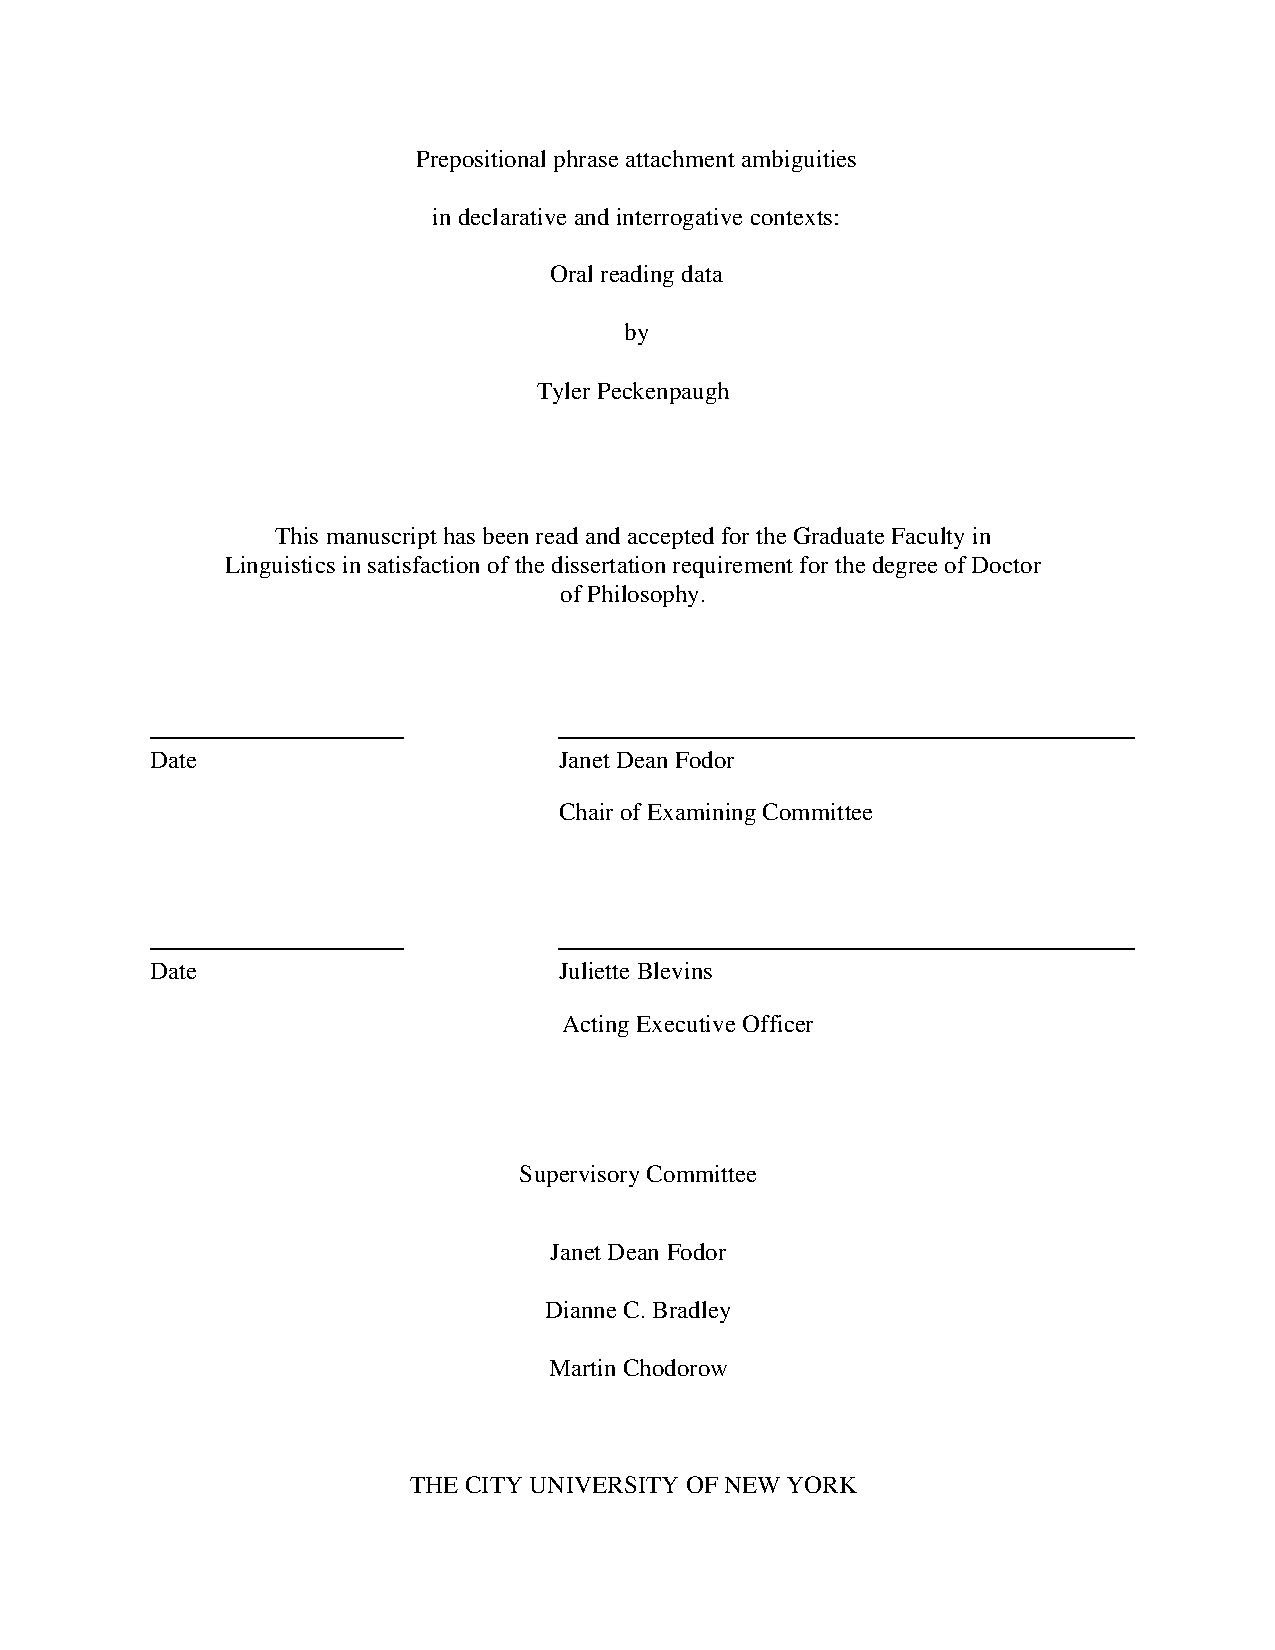
\includepdf[pages=1]{approval-page.pdf}

\pagebreak

ABSTRACT

\vspace{0.25in}

Prepositional phrase attachment ambiguities in declarative and interrogative contexts: Oral reading data

\vspace{0.25in}

by 

Tyler Peckenpaugh

\vspace{0.5in}

\raggedright 
Advisor: Janet Dean Fodor

\vspace{0.5in}


\setlength\parindent{24pt}\setlength{\parskip}{0.0pt plus 1.0pt}

Certain English sentences containing multiple prepositional phrases (e.g., \textit{She had planned to cram the paperwork in the drawer into her briefcase}) have been reported to be prone to mis-parsing of a kind that is standardly called a “garden path.” The mis-parse stems from the temporary ambiguity of the first prepositional phrase (PP1: \textit{in the drawer}), which tends to be interpreted initially as the goal argument of the verb cram. If the sentence ended there, that would be correct. But that analysis is overridden when the second prepositional phrase (PP2: \textit{into her briefcase}) is encountered, since the \textit{into} phrase can only be interpreted as the goal argument of the verb. Thus, PP2 necessarily supplants PP1’s initially assigned position as goal, and PP1 must be reanalyzed as a modifier of the object NP (\textit{the paperwork}).  

Interrogative versions of the same sentence structure (\textit{Had she planned to cram the paperwork in the drawer into her briefcase?}) may have a different profile. They have been informally judged to be easier to process than their declarative counterparts, because they are less susceptible to the initial garden path analysis. The study presented here represents an attempt to find a behavioral correlate of this intuitive difference in processing difficulty.

The experiment employs the Double Reading Paradigm (Fodor, Macaulay, Ronkos, Callahan, and Peckenpaugh, 2019). Participants were asked to read aloud a visually presented sentence twice, first without taking any time at all to preview the sentence content (Reading 1), and then again after unlimited preview (Reading 2). The experimental items were created in a 2 x 2 design with one factor being Speech Act (declarative vs. interrogative) and the other being PP2 Status, i.e., PP2 could only be an argument of the verb (Arg), as above, or else PP2 could be interpreted as a modifier (Mod) of the NP within the preceding PP, as in \textit{She had / Had she planned to cram the paperwork in the drawer of her filing cabinet(?)}.  

Participants' recordings of Reading 1 and Reading 2 were subjected to prosodic coding by a linguist who was naive to the research question. Distributions of prosodic boundaries were statistically analyzed to extract any significant differences in prosodic boundary patterns as a function of Speech Act, Reading, or PP2 Status. Logistic mixed effect regression models indicated, as anticipated, a significant effect of PP2 Status across all analyses of prosodic phrasing, and a significant effect of Reading for both analyses of prosodic phrasing that included boundary strength. Speech Act was a significant predictor in one of prosodic phrasing, but the hypothesized interaction (between Speech Act and PP2 Status) was not significant in any model.

Another analysis concerned the amount of time a participant spent silently studying a sentence after Reading 1 to be confident they had understood it before reading it aloud again (Reading 2). The time between readings is referred to as the inter-reading time (IRT). It was assumed that a longer IRT signifies greater processing difficulty of the sentence. Thus, IRT was hypothesized to provide a behavioral correlate of the intuitive judgement that the interrogative garden paths are easier to process than the declarative ones. If a correlate had been found, it would have taken the form of an interaction between the two factors (Speech Act and PP2 Status) such that the IRT difference between Arg and Mod sentence versions was smaller for interrogatives than for declaratives.  Ultimately, however, no statistically significant interaction between Speech Act and PP2 Status was found. 

Further studies seeking behavioral evidence of the informal intuition motivating this research are proposed. Also offered are possible explanations for why the intuition is apparently so strong for some English speakers, and why, if so, it is not reflected in IRT. Significant ancillary findings are that interrogatives are in general more difficult to process than corresponding declaratives. Also, inter-reading time (IRT) in the Double Reading paradigm is confirmed as a useful measure of sentence processing difficulty given that within the declarative sentences, the garden-path (Arg) versions showed significantly longer IRTs than the non-garden-path (Mod) versions. 

\pagebreak

\centering 

ACKNOWLEDGEMENTS

\vspace{0.5in}

\raggedright

\setlength\parindent{24pt}\setlength{\parskip}{0.0pt plus 1.0pt}

The completion of this dissertation would have been impossible without the help of my friends, family, colleagues, and most of all, my committee of advisors. The timing of its completion could not have been more difficult for me or for the chair of my committee, Janet Dean Fodor. To Janet, I say: thank you for your endurance, your wisdom, and your patience. I'm so grateful that you have stuck with me through all the hardship we have both dealt with this past year.

Much of the burden that stemmed from the difficult timing fell onto my second adviser, Dianne Bradley. To Dianne, I say: thank you for your tireless effort, your support, and your encouragement. There is absolutely no possible world in which I completed this dissertation without you. Your efforts, your wit, and your timely comfort kept me going when I thought I could go no further.
	
It has been said that linguists are bad at math. This shortcoming is true of me, if not all my fellows. The burden of this fell mostly upon my third adviser, Martin Chodorow. To Martin, I say: thank you for your kindness, your readiness to explain, and your forgiveness for my many mistakes. You have always been ready to help, offer a kind word, and reassure me. I knew almost nothing about statistics before I met you, and I am grateful for all you've taught me.

I am also indebted in particular to my closest friend and partner, Tally Callahan. She endured many restless nights, grumpy days, unhinged panic attacks, and worse. Thank you, Tally, for helping me see this through.

In a more practical way, I am indebted to Eva Fern\'{a}ndez and Nathacia Lucena. Without them, data collection would have been infinitely more difficult. Thank you for the use of your lab! And, to Bill Haddican, for his advice on handling the syntax of the construction I studied. 

I must also profusely thank my informants: Sita Carraturo, who surely went above and beyond; Danielle Ronkos, who has also been an important source of support; and Rachel Zane, who helped me despite my nonsense. Special thanks to my brother-in-law, Kurtiss Hare, for his help with my Python coding.

I also want to thank my parents and my sister for their love and encouragement. It was an extremely difficult time for us as a family, and especially for my father. For your understanding of the limitations on my time that writing this dissertation entailed, thank you. 

Also, thank you to my friends Corbin Neuhauser and Kathryn O’Shields for their input on the matters at large, as well as their camaraderie. Likewise, Burke Blackman, Pablo Gonz\'{a}lez, and Michael Madden, for friendship and encouragement.

Last but not least, thank you to Anne Lobeck and Kristen Denham, without whom I would never have discovered my passion for this field. Thank you, and keep inspiring your students!

\pagebreak

{
\setcounter{tocdepth}{1}
\tableofcontents
}
\listoftables
\listoffigures
\pagebreak

\setlength\parindent{24pt}\setlength{\parskip}{0.0pt plus 1.0pt}

\pagenumbering{arabic}

\hypertarget{introduction-and-background}{%
\chapter{Introduction and background}\label{introduction-and-background}}

\setlength\parindent{24pt}\setlength{\parskip}{0.0pt plus 1.0pt}

This paper presents a study on human sentence processing, or parsing, and on the parsing of a particular sort of ambiguity. Parsing is assumed to be the projection of structure by a reader or listener over a string of words (which lacks inherent structure). Following the models of parsing developed by, e.g., Kimball (1973), Frazier \& Fodor (1978), and Frazier (1979), this study assumes that parsing is done online , (i.e., during listening to or reading the word string) with the aim that most material is incorporated into the structure being built as soon as it is encountered. This can lead to mis-parses, where the parser has guessed wrong about how to incorporate a temporarily ambiguous phrase in the input, which becomes apparent when subsequent material is encountered which cannot be incorporated into the resulting structure. This sort of parsing crash is called a ``garden path.'' When it happens, the parser must reanalyze the material that had so far been processed, in order to arrive at a structure that can accommodate both the new and the old material grammatically.

In short: ``Garden path'' effects occur when temporarily ambiguous sentence resolves in such a way that the structure initially preferred by the parser is incompatible with how the sentence actually continues. These parsing errors have traditionally been attributed to structurally-driven parsing biases (cf.~Kimball, 1973; Frazier, 1979; Frazier \& Fodor, 1978) which ignore semantic content on the first pass. Frazier (1979) formulates several of these structural preferences, including the following two which are widely accepted in one form or another:

\begin{enumerate}
\def\labelenumi{(\arabic{enumi})}
\item
  \emph{Minimal attachment} \linebreak\nopagebreak
  Attach incoming material into the phrase-marker being constructed using the fewest nodes consistent with the well-formedness rules of the language under analysis (Frazier, 1979, p. 24)
\item
  \emph{Late closure} \linebreak\nopagebreak
  When possible, attach incoming material into the clause currently being parsed (Frazier, 1979, p. 20)
\end{enumerate}

Because these strategies ignore semantic and pragmatic plausibility and the parser typically does not know what material might occur further on in the word string, mis-parses at temporarily ambiguous regions can occur. Minimal Attachment (MA) is important to the present study.

An example is the commonly studied garden path sentence, ``The horse raced past the barn fell'' (Bever, 1970). Here, the initial parse incorrectly assumes that the matrix subject is the unmodified NP \emph{the horse}, per Minimal Attachment, and takes the matrix verb to be \emph{raced}, as in the sentence, \emph{The horse raced past the finish line}.

\begin{enumerate}
\def\labelenumi{(\arabic{enumi})}
\setcounter{enumi}{2}
\tightlist
\item
  The horse raced past the barn fell. (Bever, 1970)

  \begin{enumerate}
  \def\labelenumii{\alph{enumii})}
  \tightlist
  \item
    {[}\textsubscript{S} {[}\textsubscript{NP} The horse{]} {[}\textsubscript{VP} raced past the barn{]}{]}   ???   {[}\textsubscript{VP} fell{]}
  \item
    {[}\textsubscript{S} {[}\textsubscript{NP} The horse raced past the barn{]} {[}\textsubscript{VP} fell{]}{]}
  \end{enumerate}
\end{enumerate}

An attempted parse resulting in structure (3 a) crashes, as it is not possible to incorporate the final word \emph{fell} in a grammatical way. Reanalysis is required, with the grammatical parse being (3 b) where the matrix subject is \emph{the horse raced past the barn}, a noun phrase (NP) in which \emph{the horse} is modified by a reduced relative clause \emph{raced past the barn}. Then \emph{fell} can be incorporated as the matrix verb of the sentence, with a structure comparable to, \emph{The horse (that was) raced past the barn was hungry}.

The study reported in this dissertation is concerned with sentences that contain a temporarily ambiguous prepositional phrase (PP1), followed by another (PP2) which causes the initial parse to crash. Specifically, it is expected that PP1 in an example such as (4) will initially be interpreted as the goal of \emph{cram}, but that parse will fail when it is realized that PP2 (\emph{in his briefcase}) cannot plausibly modify \emph{drawer}. Instead, PP1 will have to modify \emph{paperwork} so that PP2 can be the goal argument of \emph{cram}.

\begin{enumerate}
\def\labelenumi{(\arabic{enumi})}
\setcounter{enumi}{3}
\item
  He had planned to cram the paperwork {[}\textsubscript{PP1} in the drawer{]} {[}\textsubscript{PP2} in his briefcase{]}.
\item
  He had planned to cram the paperwork {[}\textsubscript{PP1} in the drawer {[}\textsubscript{PP2} of his filing cabinet{]}{]}.
\end{enumerate}

This contrasts with the sentence in (5), where PP2 can plausibly modify \emph{drawer} and so the parse where the PP1 \emph{in the drawer} is the goal argument is acceptable, and \emph{of his filing cabinet} is incorporated as a modifier within it.

\hypertarget{obs}{%
\section{Motivations for the current study}\label{obs}}

The current study was initially motivated by a phenomenon discovered by Janet Dean Fodor and Dianne Bradley, and originally reported in Peckenpaugh (2016). That observation was that a garden path sentence like (4) repeated here as (6) is, for whatever reason, not as difficult to process when presented as an interrogative, as in (7), rather than as a declarative.

\begin{enumerate}
\def\labelenumi{(\arabic{enumi})}
\setcounter{enumi}{5}
\item
  He had planned to cram the paperwork in the drawer in his briefcase.
\item
  Had he planned to cram the paperwork in the drawer in his briefcase?
\end{enumerate}

Peckenpaugh (2016) attempted to find a behavioral correlate of this intuition by examining variation in reading time for sentences like (6) and (7), but the results were inconclusive. The current study continues that line of research by testing similar sentences, while also attempting to control certain factors that may have led to Peckenpaugh (2016)'s inconclusive results. One such concern is that (6) relies on the practical implausibility of a drawer within a briefcase, i.e., on real world knowledge, in order to disambiguate the appropriate sites for PP1 and PP2. Real world knowledge and beliefs about what is or is not plausible likely vary between speakers and so may not always be effective as a trigger for reanalysis. The current study makes use of carefully constructed sentences (the criteria by which they were constructed are detailed in Section \ref{mat}) which do not rely on plausibility or pragmatics to disambiguate the PP attachment sites, but instead make use of what will be referred to as syntactic disambiguation by including a PP2 that cannot grammatically be incorporated into PP1. This is illustrated in (8) and (9).

\begin{enumerate}
\def\labelenumi{(\arabic{enumi})}
\setcounter{enumi}{7}
\item
  He had planned to cram the paperwork {[}\textsubscript{PP1} in the drawer{]} {[}\textsubscript{PP2} into his briefcase{]}.
\item
  Had he planned to cram the paperwork {[}\textsubscript{PP1} in the drawer{]} {[}\textsubscript{PP2} into his briefcase{]}?
\end{enumerate}

Note that ``syntactic disambiguation'' is the term that will be used throughout this dissertation to refer to the sort of disambiguation used in the experimental materials of the current study. Various terms might be used, e.g., ``lexical'' or ``semantic'', since the disambiguation hinges on the lexical identity and semantics of the preposition that heads PP2, i.e., \emph{into} instead of \emph{in} and what syntactic position or semantic role such a PP can be assigned. But, such distractions will not be discussed here. The change from pragmatic disambiguation in (6) and (7) to syntactic disambiguation in (8) and (9) creates an important distinction between the hypothesis tested in Peckenpaugh (2016) and the hypothesis to be tested in the current study. It cannot be assumed that the intuition about (6) and (7) necessarily extends to cases like (8) and (9), and so one of the questions the current study addresses is whether the apparent greater ease of processing a question than a declarative can be shown to extend to syntactically disambiguated cases that are similar to the pragmatically disambiguated cases for which the observation was first made. In order to keep a clear focus on this small but potentially important difference, a convention will be adopted throughout this document where the intuited amelioration of the garden path effect in pragmatically disambiguated cases is referred to as the 2016 Intuition, while the possibility that the 2016 Intuition extends to syntactically disambiguated cases is referred to as the Current Hypothesis.

\begin{enumerate}
\def\labelenumi{(\arabic{enumi})}
\setcounter{enumi}{9}
\item
  \emph{The 2016 Intuition:} Certain pragmatically disambiguated prepositional phrase (PP) attachment ambiguities which are difficult to parse in the declarative are less difficult to parse when presented as yes-no interrogatives (e.g., \emph{The nanny sat the cranky little boy in the stroller on the swing}, vs.~\emph{Did the nanny seat the cranky little boy in the stroller on the swing?}).
\item
  \emph{The Current Hypothesis:} The 2016 Intuition may be extensible to PP attachment ambiguities that are syntactically disambiguated rather than pragmatically disambiguated (e.g., \emph{He had planned to cram the paperwork in the drawer into his briefcase}, vs.~\emph{Had he planned to cram the paperwork in the drawer into his briefcase?}).
\end{enumerate}

In addition to exploring the possible extensibility of the 2016 Intuition, the current study addresses what property or properties of polar questions might lead to an easier parsing of garden paths, or at least to the perception that they are easier to parse when compared to declaratives. Because there are minimal differences between the polar question and declarative versions of these sentences, it seems likely that the cause lies in one of two domains: either the prosodic changes triggered by the use of question intonation, or the pragmatic and semantic properties that are not shared across the versions.

An obvious reflex of the former possibility is another question: how are the various versions of these sentences actually pronounced, prosodically? The reported study seeks to answer this, but while the recordings collected provide some insight, more work is likely needed to provide a fully satisfactory answer.

Likewise, the latter possibility raises the question: exactly what are the semantic and pragmatic differences between a polar question and its declarative counterpart? This question has been approached in the theoretical literature (see, e.g.~Fiengo (2007)). Nevertheless, it remains to be determined how those properties could lead to an easier or more difficult parsing process.

\hypertarget{mech}{%
\section{Structural overview of the ambiguity relevant to this study}\label{mech}}

The 2016 Intuition and the current hypothesis are both concerned with a temporarily ambiguous sequence of PPs at the end of a sentence. The example in (12) shows a pragmatically disambiguated sentence with an argument-PP2.

\begin{enumerate}
\def\labelenumi{(\arabic{enumi})}
\setcounter{enumi}{11}
\tightlist
\item
  He crammed the paperwork in the drawer in his briefcase.

  \begin{enumerate}
  \def\labelenumii{\alph{enumii}.}
  \tightlist
  \item
    \(\#\) \ldots{} {[}\textsubscript{VP} crammed {[}\textsubscript{NP} the paperwork{]} {[}\textsubscript{PP1} in {[}\textsubscript{NP} the drawer {[}\textsubscript{PP2} in his briefcase{]}{]}{]}
  \item
    \(\checkmark\) \ldots{} {[}\textsubscript{VP} crammed {[}\textsubscript{NP} the paperwork {[}\textsubscript{PP1} in {[}\textsubscript{NP} the drawer {]}{]} {[}\textsubscript{PP2} in his briefcase{]}{]} \linebreak\nopagebreak
    \emph{``\(\#\)'' indicates a structure with an implausible reading}
  \end{enumerate}
\end{enumerate}

The initial parse is expected to be (12 a) because of a bias (due to Minimal Attachment, or some variation thereof, see (1) above), which favors a structure where the first PP attaches into the verb phrase (VP) as an argument of the verb, i.e., {[}\textsubscript{VP} V NP PP1{]} with PP1 denoting the goal, which leaves nowhere for the second PP to attach but as a modifier of the noun phrase (NP) inside PP1 ({[}\textsubscript{PP1} \emph{under} {[}\textsubscript{NP} \emph{the sofa} {[}\textsubscript{PP2} \emph{in the wastebasket}{]}{]}{]}). This initial parse (12 a) is pragmatically implausible, since sofas are generally not found inside wastebaskets. Structural reanalysis is required to bring about the only plausible parse (12 b), where PP1 attaches as a modifier of the direct object NP and so allows PP2 to attach to the VP as a goal argument, resulting in a structure such as {[}\textsubscript{VP} V {[}\textsubscript{NP} N PP1{]} PP2{]}, i.e., where it is the paperwork in the drawer that is being crammed in his briefcase.

Regarding the ambiguity of the preposition \emph{in} which heads PP1 in (13) below: Gehrke (2006) discusses its semantics and notes that it has two interpretations in some varieties of English, including standard American English. These interpretations accord with the ambiguity of the two possible attachment sites for PP1 in examples such as (13) below. The standard reading of \emph{in} in this context is locative, as in (13 a), where that reading is forced by the unambiguous directional reading of \emph{into} in PP2, which must ultimately fill the goal argument position. In contexts of directed motion (as with a verb like \emph{cram} in example (13)), however, a directional reading of \emph{in} is licensed; thus, in (13 b) where PP2 is headed by \emph{of}, which cannot be directional and so cannot be the goal argument, PP1 is interpreted as the goal. (Gehrke notes that English is exceptional among Germanic languages with respect to the ambiguity of \emph{in}, which typically require some form of overt marking for the directional interpretation.)

\begin{enumerate}
\def\labelenumi{(\arabic{enumi})}
\setcounter{enumi}{12}
\tightlist
\item
  \textbf{PP2 attachment status} \linebreak\nopagebreak

  \begin{enumerate}
  \def\labelenumii{(\alph{enumii})}
  \tightlist
  \item
    \emph{PP2 Argument} (Arg) \linebreak\nopagebreak
    He had planned to cram the paperwork {[}\textsubscript{PP1} in\textsubscript{Locative} the drawer{]} {[}\textsubscript{PP2} into\textsubscript{Directional} his briefcase{]}.
  \item
    \emph{PP2 Modifier} (Mod) \linebreak\nopagebreak
    He had planned to cram the paperwork {[}\textsubscript{PP1} in\textsubscript{Directional} the drawer {[}\textsubscript{PP2} of\textsubscript{Genitive} his filing cabinet{]}{]}.
  \end{enumerate}
\end{enumerate}

For clarity in what follows, the current study categorizes these sentences into two categories based on the status of the PP2 they contain: (a) cases where PP2 is an argument of the verb are referred to as Arg-type sentences, and (b) cases where PP2 is a modifier of the preceding noun are called Mod-type sentences; see (13) above. As noted, it is the Arg sentences that are generally reported to be garden paths, because PP2 must fill the goal role that PP1 is initially expected to have filled, as just discussed. Mod sentences are not likely to result in a garden path, because PP2 can modify the NP within PP1 to become part of the goal, and therefore need not disrupt PP1's attachment as the goal.

In order for the differing parsing process for (13 a) and (13 b) to be explained by a strictly structure based model of parsing, certain assumptions have to be made about the syntax. A simple way to achieve it is to assume that all arguments of a verb are syntactic sisters to the verb, resulting in a three-way branching VP for ditransitive verbs such as \emph{cram} ; see Figure \ref{fig:threetree}. In this case, in order to avoid postulating extra nodes that would be required for PP1 to be a modifier of the object NP, Minimal Attachment dictates that PP1 should be assumed to fill the verb's goal argument slot. Note that while both \emph{into} and \emph{onto} are employed as disambiguator for Arg sentences, for the sake of clarity, discussion throughout this dissertation are limited to examples of \emph{into}.

The most pronounced structural difference between the two structures is that in the sentence with a modifier-PP2 (Mod) the major disjuncture comes fairly early, just after the object NP \emph{the newspapers}. For the sentences with argument-PP2s (Arg), the major disjuncture is later, just after PP1 (\emph{under the sofa}).

\begin{figure}
  \centering
  \begin{forest}
    where n children=0{tier=word,font=\normalsize}{}
    \footnotesize
    [VP
      [V]
      [NP]
      [PP]
    ]
  \end{forest}
  \caption{Illustrative syntactic tree of a ternary-branching VP.}
  \label{fig:threetree}
\end{figure}

It bears mentioning that Minimal Attachment as defined by Frazier (1979) is somewhat at odds with recent developments in syntactic theory, e.g., obligatory binary branching; three-way branching is proscribed (cf.~Chomsky, 2014, p. 62). As originally postulated, Minimal Attachment relies on a verb with multiple internal arguments incorporating each of those arguments as a sister (i.e., a ternary branching structure as in Figure \ref{fig:threetree} above).

Within current theories of syntax, where branching is obligatorily binary, NP and PP cannot both be syntactic sisters of the verb, so structures as bracketed in (12) are impossible. Instead, the structures would be as shown in Figures \ref{fig:modTree} and \ref{fig:argTree} below\footnote{Note that when the internal structure of an NP is not relevant (no PP is within it) it is not drawn in these figures, i.e., {[}NP newspapers{]} is shorthand for {[}NP {[}N' {[}N newspapers{]}{]}{]}.}, in which case it becomes less clear that the VP attachment site for PP1 actually creates fewer nodes than the lower NP attach as per Minimal Attachment. Nonetheless, empirical studies by, e.g., Rayner, Carlson, \& Frazier (1983), Clifton, Speer, \& Abney (1991), and others, show that a preference for VP attachment of a PP does exist in contexts such as the current study addresses, whether that preference is best explained by Minimal Attachment, or a preference for arguments over non-arguments, or some other mechanism.

\begin{figure}[!hbtp]
  \centering
  \begin{forest}
    where n children=0{tier=word,font=\normalsize}{}
    \footnotesize
    [\dots
      [VP 
        [V' 
          [V' 
            [V [cram]] 
            [DP 
              [D' 
                [D [the]] 
                [NP [newspapers]]
                ]
              ]
            ]
          ]
          [PP1$_{Arg}$
            [P' 
              [P [under]] 
              [DP 
                [D'
                  [D [the]] 
                  [NP
                    [N'
                      [N' [N [sofa]]]
                      [PP2$_{Mod}$
                        [P'
                          [P [from]] 
                          [DP 
                            [D' 
                              [D [the]] 
                              [NP [thrift store]]
                            ]
                          ]
                        ]
                      ]
                    ]
                  ]
                ]
              ]
            ]
          ]
        ]
      ]
    ]
  \end{forest}
  \caption{Syntactic tree of an illustrative example sentence with a (temporarily) PP1 and a modifier-PP2 (Mod).}
  \label{fig:modTree}
\end{figure}

\begin{figure}[!hbtp]
  \centering
  \begin{forest}
    where n children=0{tier=word,font=\normalsize}{}
    \footnotesize
    [\dots
      [VP 
        [V' 
          [V' 
            [V [cram]] 
            [DP 
              [D' 
                [D [the]] 
                [NP 
                  [N' 
                    [N [newspapers]]
                  ] 
                  [PP1$_{Mod}$ 
                    [P'
                      [P [under]] 
                      [DP 
                        [D' 
                          [D [the]] 
                          [NP [sofa]]
                        ]
                      ]
                    ]
                  ]
                ]
              ]
            ]
          ]
          [PP2$_{Arg}$
            [P' 
              [P [into]] 
              [DP 
                [D'
                  [D [the]] 
                  [NP [wastebasket]]
                ]
              ]
            ]
          ]
        ]
      ]
    ]
  \end{forest}
  \caption{Syntactic tree of an illustrative example sentence with a (temporarily) ambiguous PP1 and an argument-PP2 (Arg).}
  \label{fig:argTree}
\end{figure}

Setting the particularities of syntactic theory aside now,, an appeal can be made to a psycho-linguistic distinction added to parsing theory in \emph{Construal} (Frazier \& Clifton, 1996): that of primary vs.~non-primary relations.

\begin{enumerate}
\def\labelenumi{(\arabic{enumi})}
\setcounter{enumi}{13}
\tightlist
\item
  "Primary phrases and relations include

  \begin{enumerate}
  \def\labelenumii{\alph{enumii})}
  \tightlist
  \item
    The subject and main predicate of any (+ or -) finite clause
  \item
    Complements and obligatory constituents of primary phrases"\linebreak\nopagebreak
    (Frazier \& Clifton, 1996, p. 41)
  \end{enumerate}
\end{enumerate}

This additional contrast is independently motivated: Frazier and Clifton illustrate this by way of relative clause (RC) attachment in constructions like (15).

\begin{enumerate}
\def\labelenumi{(\arabic{enumi})}
\setcounter{enumi}{14}
\tightlist
\item
  The journalist interviewed {[}\textsubscript{NP1} the daughter\textsubscript{i}{]} of {[}\textsubscript{NP2} the colonel\textsubscript{j}{]} {[}\textsubscript{RC} who\textsubscript{i/j} had an accident{]}. (Frazier \& Clifton, 1996, p. 71).
\end{enumerate}

The RC in (15) can modify either NP1, \emph{the daughter}, or NP2 \emph{the colonel}. Late Closure(see (2), above) predicts a consistent preference for local attachment of the RC in (15), i.e., the structure where the RC modified NP2. This is because Late Closure dictates that the NP2 phrase not be closed until necessary, i.e., until material that cannot, for one reason or another, be incorporated into that phrase is encountered. Since the RC can modify NP2, Late Closure predicts that it will (Frazier \& Clifton, 1996). Instead, what a number of empirical studies (e.g., Clifton, 1988; Cuetos \& Mitchell, 1988) find is a pattern where the preferred structure depends on the relationship between NP1 and NP2. Frazier \& Clifton (1996) describe five categories of relationship, and a gradient of preferred RC attachment, from NP1 preference to NP2 preference.

\begin{enumerate}
\def\labelenumi{(\arabic{enumi})}
\setcounter{enumi}{15}
\tightlist
\item
  \textbf{RC Attachment by NP1-NP2 relation} (Frazier \& Clifton, 1996, p. 31)

  \begin{enumerate}
  \def\labelenumii{\alph{enumii}.}
  \tightlist
  \item
    \emph{Material} \linebreak\nopagebreak
    The table of wood {[}\textsubscript{RC} that was from Galicia{]}
  \item
    \emph{Quantity} \linebreak\nopagebreak
    The glass of wine {[}\textsubscript{RC} you liked{]}
  \item
    \emph{Relational} (friend, enemy, son, and other argument taking NPs, e.g., picture-NPs) \linebreak\nopagebreak
    The son of the woman {[}\textsubscript{RC} that was dying{]}
  \item
    \emph{Possessive} \linebreak\nopagebreak
    The car of the company {[}\textsubscript{RC} that was falling apart{]}
  \item
    \emph{Non-accompaniment} with \linebreak\nopagebreak
    The girl with the hat {[}\textsubscript{RC} that looked funny{]}
  \end{enumerate}
\end{enumerate}

Frazier \& Clifton (1996) cite experimental studies showing that (16 a-b) type configurations favor NP1 RC attachment, (16 e) type configurations favor NP2 RC attachment, while (16 c-d) are intermediate. They argue that this gradient cannot be readily explained by structural parsing, and instead they make use of a mechanism they call association. RCs, rather than being immediately slotted into a tree in a specific way, are \emph{associated} with a thematic domain, i.e., the maximal projection of whatever lexical item last assigned theta-roles, together with associated functional projections. In such cases, the parsing decision can be made later, which allows the syntactic structure to be decided after semantic information becomes available. The RC can ultimately modify whichever member of the thematic domain is appropriate.

The factor that determines whether \emph{association} or structural parsing is appropriate is the distinction between primary vs.~non-primary relations. Frazier and Clifton's formalization of this distinction is given in their definition of primary relations in (14) above, and all other relations are non-primary.

RC attachment undergoes association because relative clauses are by definition modifiers, and the relationship between a modifier and whatever it modifies is a non-primary relation. Returning now to the PP-attachment construction that this study is concerned with, the argument vs.~modifier distinction is precisely what distinguishes the two possible roles of PP2 shown in (13), repeated here as (17).

\begin{enumerate}
\def\labelenumi{(\arabic{enumi})}
\setcounter{enumi}{16}
\tightlist
\item
  \textbf{PP2 types}

  \begin{enumerate}
  \def\labelenumii{\alph{enumii}.}
  \tightlist
  \item
    \emph{PP2 Modifier} (Mod)
    He had planned to cram the paperwork {[}\textsubscript{PP1} in the drawer {[}\textsubscript{PP2} of his filing cabinet{]}{]}.
  \item
    \emph{PP2 Argument} (Arg)
    He had planned to cram the paperwork {[}\textsubscript{PP1} in the drawer{]} {[}\textsubscript{PP2} into his briefcase{]}.
  \end{enumerate}
\end{enumerate}

The infinitival clause headed by \emph{cram} is a primary phrase, and so its obligatory constituents hold primary relationships with \emph{cram}. As such, association is not available as a mechanism and structural parsing must occur, without semantic information being available. Thus, PP1 is initially interpreted as the goal argument of \emph{cram}. Then, in the case of (17 a), when PP2 is encountered, PP1 must be removed from that syntactic position and be reanalyzed as a modifier of the object NP in order to allow PP2 to fill the goal argument position. In the case of (17 b), no reanalysis is necessary because PP2 (\emph{of his filing cabinet}) is not an argument (\emph{of} is not directional) and thus can modify \emph{the drawer}, not needing to dislodge PP1.

\hypertarget{intg}{%
\section{Interrogativity}\label{intg}}

This section returns to the questions raised by the 2016 Intuition discussed in Section \ref{obs} about why certain garden paths of the sort just discussed might appear to be easier to parse in interrogative constructions than in otherwise similar declarative ones (see examples (18) and (19)).

\begin{enumerate}
\def\labelenumi{(\arabic{enumi})}
\setcounter{enumi}{17}
\tightlist
\item
  He had planned to cram the paperwork {[}\textsubscript{PP1} in the drawer{]} {[}\textsubscript{PP2} in his briefcase{]}.
\item
  Had he planned to cram the paperwork {[}\textsubscript{PP1} in the drawer{]} {[}\textsubscript{PP2} in his briefcase{]}?
\end{enumerate}

What exactly differs between (18) and (19)? Syntactically, very little: the position of the subject \emph{he} and the auxiliary \emph{had} have been reversed, but the words that follow are identical.

The semantic, or perhaps more accurately pragmatic, differences between (18) and (19) lie with the presuppositions the sentences carry with them, which may vary with the placement of focus, marked phonologically in spoken language. The exact phonetic properties of focus, and the semantic and syntactic consequences of it, are widely studied and debated. For an excellent overview of the topic, see Ladd (2008), pp.213-23. The assumptions made about focus in this dissertation concern English only, and are more or less compatible with a Focus-to-Accent model as described by Ladd, which distinguishes ``the semantic/pragmatic notion `focus' from the phonetic/phonological notion `accent' and -- crucially -- {[}\ldots{]} allows focus to apply to portions of utterances larger than individual words'' (Ladd, 2008, p. 217). This results in sentential stress being split into two related but independent components: (a) where focus lies within the sentence, and (b) how focus is conveyed with regard to the location of a phonological accent.

The declarative in (18) has few presuppositions beyond the existence of the actors and objects involved (the referents of \emph{he}, \emph{paperwork}, \emph{drawer} and \emph{briefcase}), and that these actors and objects can be involved in \emph{cramming}. The presuppositions of (19) are different from those of (18): for instance, a yes/no question additionally presupposes that the listener does or may know the answer to the question. Further presuppositions may exist, depending on where the focus lies within the sentence.

Focus in a declarative like (18) is typically wide, i.e., no element is having special attention called to it. A polar question like (19), however, will often receive narrower focus on one word or phrase, so that when uttered, that word or phrase is more prominent than the others. The focused element becomes the part of the sentence that the question is about. Focus can fall on any of the lexical or referential elements in the sentence (subject, auxiliary verb, matrix verb, infinitival verb, object NP, or the NP of either PP1 or PP2, or any part of one of these). In the examples below, a small sample of possible focus locations are shown, with words in all capital letters indicating verbal emphasis signifying focus.

\begin{enumerate}
\def\labelenumi{(\arabic{enumi})}
\setcounter{enumi}{19}
\item
  \begin{enumerate}
  \def\labelenumii{\alph{enumii}.}
  \tightlist
  \item
    HAD he planned to cram the paperwork {[}\textsubscript{PP1} in the drawer{]} {[}\textsubscript{PP2} into his briefcase{]}?
  \item
    Had HE planned to cram the paperwork {[}\textsubscript{PP1} in the drawer{]} {[}\textsubscript{PP2} into his briefcase{]}?
  \item
    Had he planned to cram the paperwork {[}\textsubscript{PP1} in the DRAWER{]} {[}\textsubscript{PP2} into his briefcase{]}?
  \item
    Had he planned to cram the paperwork {[}\textsubscript{PP1} in the drawer{]} {[}\textsubscript{PP2} into HIS briefcase{]}?
  \end{enumerate}
\end{enumerate}

In (20 a), with focus on the auxiliary, the question encompasses the entire proposition, and asks whether or not it is true. In this case, there are not any additional presuppositions when compared to the declarative counterpart of the sentence. In (20 b), with focus on \emph{he}, the question is asking about whether the referent of \emph{he} is the actor who performed the action described; in this case, the entire predicate is presupposed: someone had planned to cram the paperwork in the drawer into his briefcase, but was it him? In (20 c), with focus on \emph{drawer}, the question is instead about which paperwork this is all happening to: the paperwork that is in the drawer, or some other stack of paperwork? In this case, it is presupposed that the referent of \emph{he} was the one who had planned to cram some paperwork into his briefcase, and only the exact referent of \emph{the paperwork} is not presupposed. For each other location of focus, the presuppositional content is similarly complementary to whichever element is focused and therefore being asked about.

This set of pragmatic differences between (18) and (19) might be the source of the 2016 Intuition that (19) is easier to comprehend than (18), but it is not it is not immediately clear why that would be (see Section \ref{sem} for one way in which it might), and that is not the only possibility. Another significant difference between the two sentences is the rhythm and intonational melody (which together make up the prosody). While dialects of English may differ prosodically, there is typically a difference in melody between a declarative and a question, and in many American English dialects, the interrogative is pronounced with a final rise, while the declarative exhibits just a series of down-steps. This difference is the one that the current study explores, to see if it can be shown to correlate with a difference in processing difficulty in syntactically disambiguated declarative and interrogative PP-attachment garden paths, and by extension lend insight into the 2016 Intuition.

\hypertarget{prosody-of-questions-vs.-declaratives}{%
\section{Prosody of questions vs.~declaratives}\label{prosody-of-questions-vs.-declaratives}}

In pursuing the possibility that it is the prosody of polar interrogatives which creates the 2016 Intuition that motivated this study it is important to consider the details of question intonation actually sounds like. It is generally agreed that in American English, the intonation of a polar question exhibits a final rise. This has been confirmed in corpus studies such as Hedberg, Sosa, \& Görgülü (2017) who found that 79.8\% of the 410 American English yes/no questions in their study (ten-minute phone conversations from the CallHome Corpus of American English and the Fisher English Corpus) had a ``low-rise nuclear contour'' (L*H-H\%, L*H-\(\uparrow\)H\%, or L*L-H\%)\footnote{Hedberg et al. (2017) use \(\uparrow\) to indicate an up-step, which is not standardly transcribed with ToBI.}. In their ToBI notation, a tone T is coded either L for low or H for high; T* is anchored to the stressed syllable, and T- and T\% are boundary tones (intermediate phrase boundary and intonational phrase boundary respectively). See \emph{Guidelines for ToBI labeling} (Beckman \& Ayers, 1997) for a more thorough explanation of ToBI. An additional 10.7\% of the Hedberg et al. (2017) data had a ``high-rise nuclear contour'' (the authors categorize the following tunes as high-rise nuclear contours: H*H-H\% or !H*H-H\%). That leaves only 9.5\% spread across the other 5 categories (High-fall, Rise-fall, Low-fall, Fall-rise, and Level). Only 5.6\% of the total data showed any sort of falling contour. According to the authors' analyses, final high-rise contours occur on the final main stress of a sentence and thereafter. In the case of the types of sentences examined in the current study, that would result in a rising contour on the head noun of the final PP as in (21), regardless of whether the final PP is a Mod or an Arg.

\begin{enumerate}
\def\labelenumi{(\arabic{enumi})}
\setcounter{enumi}{20}
\tightlist
\item
  Did Jed cram the newspapers under the sofa in the {[}\textsubscript{L*H-H\%} guestroom{]}?
\end{enumerate}

The need to prepare for that final rising tone might make a prosodic break before the PP more likely, and thus ease reanalysis or even encourage a different prosodic chunking which might encourage argument attachment. This possibility is revisited and more fully explained in Section \ref{prep}.

The prosodic structures observed in the data collected for the current study are discussed in \ref{results-prosody}. For discussion of what constitutes a prosodic boundary, see e.g., Streeter (1978) and Salverda, Dahan, \& McQueen (2003).

\hypertarget{prosyn}{%
\section{Prior studies of prosodic effects on syntactic parsing}\label{prosyn}}

A number of studies have shown that in listening to speech, prosodic cues help reduce the frequency with which incorrect parsing (i.e., a garden path) occurs. For example, Kjelgaard \& Speer (1999) conducted a study using digital manipulation of recorded speech to create three versions of sentences containing a temporary ambiguity which could result in a garden path. They recorded speakers saying sentences with natural prosody, such as the following pair (not bracketed in presentation to the speakers):

\begin{enumerate}
\def\labelenumi{(\arabic{enumi})}
\setcounter{enumi}{21}
\tightlist
\item
  {[}When Roger leaves{]} the house is dark. (Early closure)
\item
  {[}When Roger leaves the house{]} it's dark. (Late closure)
\end{enumerate}

They then cross-spliced these together to make several versions. One version had prosodic cues which cooperated with the intended reading of the sentence; another aimed to have ``neutral'' prosody; and the third used intentionally misleading prosody which favored the garden path. The initial fragment of each (the portion from the beginning of the sentence to the word \emph{house} in (22) and (23)) was then presented to participants who were asked to agree or disagree with whether a visually presented word, either \emph{is} or \emph{it's} was likely to be the next word in the sentence. Participants gave more accurate and speedier judgments when the visually presented word was compatible with the structure indicated by the prosodic cues. The results of this study, as well as a growing body of literature, suggest that information can indeed be used by the parser in making processing decisions.

Fodor (2002) invoked prosody in an explanation of differing relative clause attachment preference across language first pointed out by Frazier \& Clifton (1996) and discussed above in Section \ref{mech}. This specifically concerns sentences such as English (24) and Spanish (25):

\begin{enumerate}
\def\labelenumi{(\arabic{enumi})}
\setcounter{enumi}{23}
\tightlist
\item
  Someone shot the servant\textsubscript{N1} of the actress\textsubscript{N2} {[}\textsubscript{RC} who was on the balcony{]}.
\item
  Alguien disparó contra la criada\textsubscript{N1} de la actriz\textsubscript{N2} {[}\textsubscript{RC} que estaba en el balcón{]}.
\end{enumerate}

The relative clause in (24) \emph{who was on the balcony}, can attach either low/locally (modifying N2), making it \emph{the actress} who was \emph{on the balcony}, or high/non-locally (modifying N1) so that it is \emph{the servant} who was \emph{on the balcony}. While Late Closure predicts local/low attachment in these structures, Cuetos \& Mitchell (1988) found a 60\% preference for local/low attachment for the English materials, but only a 40\% preference for local/low attachment in Spanish. Thus, in apparent violation of the general preference for local/low attachment, some languages, like Spanish (also French and Russian, though not Romanian or Brazilian Portuguese, so this is not a general feature exclusive to Romance languages), prefer to attach relative clauses higher, while others more often obey Late Closure as in English (e.g., Swedish and Egyptian Arabic). Interestingly, the non-local preference in languages like Spanish is weakened in cases where the ambiguous RC is short (one prosodic word), which is compatible with its being attributable to prosodic phrasing. Fodor (2002) maintains that these tendencies exist both in listening to spoken sentences, with and without explicit prosody, and in silent reading.

Other researchers, e.g., Maynell (1999), have shown that the presence or absence of a prosodic break before an RC encourages high or low attachment respectively. Fodor leverages this in order to explain the differences in RC attachment site tendency between languages. She argues that cross-language differences can be neatly explained by linking attachment site preference to the likelihood of a prosodic break before the RC, either for length reasons (e.g., English) or due to interactions between alignment constraints and phrase length (e.g., French) (Pynte \& Prieur, 1996).

\hypertarget{pred}{%
\section{Predictions for the current study}\label{pred}}

The experimental study presented here addresses a number of issues having to do with the prosody and parsing of the construction under examination. Following e.g., Schafer, Speer, Warren, \& White (2000) as noted above, it is assumed that prosody is affected by syntax and therefore that prosody can be used to diagnose the attachment site of PP2. Before going into the predictions made, it is necessary to be clear on what the prosodic structure is that is expected, given the syntax of the construction in question. Figures \ref{fig:smallmod} and \ref{fig:smallarg} below illustrate the syntax of the VP containing the PP constructions (Mod and Arg) of relevance. These are schematic, simplified representations of the same structures shown for full sentences in Figures \ref{fig:modTree} and \ref{fig:argTree} in Section \ref{mech}.

\begin{figure}[!hb]
  \centering
  \begin{minipage}{0.45\textwidth}
      \centering
      \begin{forest}
        where n children=0{tier=word,font=\normalsize}{}
        \footnotesize
        [VP
          [V'
            [V' 
              [V]
              [N$_{OBJ}$]
            ]
            [PP1
              [NP
                [N]
                [PP2]
              ]
            ]
          ]
        ]
      \end{forest}
      \caption{Illustrative syntactic tree of the verb phrase for Mod cases.}
      \label{fig:smallmod}
  \end{minipage}\hfill
  \begin{minipage}{0.45\textwidth}
      \centering
      \begin{forest}
        where n children=0{tier=word,font=\normalsize}{}
        \footnotesize
        [VP
          [V'
            [V' 
              [V]
              [NP$_{OBJ}$
                [N$_{OBJ}$]
                [PP1]
              ]
            ]
            [PP2]
          ]
        ]
      \end{forest}
      \caption{Illustrative syntactic tree of the verb phrase for Arg cases.}
      \label{fig:smallarg}
  \end{minipage}
\end{figure}

These structures, together with the assumptions discussed in the previous section (Section \ref{prosyn}), predict linguistically motivated prosodic boundaries after the object NP in the Mod case, and after PP1 in the Arg case, setting aside boundaries that may be motivated by phrase length or other factors. In (26) and (27) ``\(\|\)'' indicates a linguistically motivated prosodic boundary.

\singlespacing

\begin{enumerate}
\def\labelenumi{(\arabic{enumi})}
\setcounter{enumi}{25}
\tightlist
\item
  \textbf{Mod pattern}
  \begingroup
  \setlength{\tabcolsep}{2pt}

  \begin{tabular}{ccccccc}
    \dots & stick & the letter & $\|$ & in the mailbox &  & of the proper stack \\
    & & \footnotesize Direct object & & \footnotesize PP1 & & \footnotesize vice president. \\
  \end{tabular}
    \endgroup
\item
  \textbf{Arg pattern}
  \begingroup
  \setlength{\tabcolsep}{2pt}

  \begin{tabular}{ccccccc}
    \dots & stick & the letter & & in the mailbox & $\|$ & onto the proper stack. \\
    & & \footnotesize Direct object & & \footnotesize PP1 & & \footnotesize PP2 \\
  \end{tabular}
    \endgroup
\end{enumerate}

\doublespacing

It also needs to be made clear at this point that the experiment reported involves two recordings of participants reading a given sentence out loud: the study reported employs the Double Reading paradigm of Fodor, Macaulay, Ronkos, Callahan, \& Peckenpaugh (2019) (more on Double Reading in Chapter \ref{method}). Therefore, predictions can be made about the prosody as a function of: declarative sentences versus interrogative sentences; Arg sentences versus Mod sentences; and about first readings versus second readings. There are two kinds of prosodic predictions at play: the speaker may produce prosodic errors, where the prosodic structure of the sentence is disfluent or unnatural in other ways, which contrasts with the other kind, prosodic mismatches, where the prosody produced is well formed but suggests a syntactic configuration that is at odds with the actual content of the sentence. For example, consider (28), where ``\(\%\)'' indicates a prosodic boundary:

\singlespacing

\begin{enumerate}
\def\labelenumi{(\arabic{enumi})}
\setcounter{enumi}{27}
\tightlist
\item
  \textbf{Prosody mismatch (Arg syntax, Mod prosody)}
  \begingroup
  \setlength{\tabcolsep}{2pt}

  \begin{tabular}{ccccccc}
    \dots & stick & the letter & $\%$ & in the mailbox & & onto the proper stack. \\
    & & \footnotesize Direct object & & \footnotesize PP1 & & \footnotesize PP2 \\
  \end{tabular}
    \endgroup
\end{enumerate}

\doublespacing

The sentence in (28) is only grammatical with Arg syntax (i.e., PP2 must be the goal argument of the verb), but might hypothetically be pronounced with the prosody of a well formed Mod sentence, with a prosodic boundary after \emph{the letter}. Given that the construction under examination is intended to mislead readers of an Arg sentence into initially mis-parsing PP1 as the goal argument, it stands to reason that prosodic errors and prosodic mismatches are more likely to occur for the Arg sentences than for the Mod sentences. These predictions are formalized as \emph{Hypothesis 1} and \emph{Hypothesis 2}.

\begin{enumerate}
\def\labelenumi{(\arabic{enumi})}
\setcounter{enumi}{28}
\tightlist
\item
  \emph{Hypothesis 1} (Prosodic Errors)\linebreak\nopagebreak
  A first reading of a sentence where PP2 is a goal argument (Arg) will be more likely to exhibit less natural prosody (e.g., more hesitation at and within the PP2 region) than either:

  \begin{enumerate}
  \def\labelenumii{\alph{enumii}.}
  \tightlist
  \item
    A first reading of a sentence where PP2 is a modifier (Mod)
  \item
    A second reading of a sentence where PP2 is a goal argument (Arg)
  \end{enumerate}
\item
  \emph{Hypothesis 2} (Prosody/Syntax Mismatch)\linebreak\nopagebreak
  A first reading of a sentence where PP2 is a goal argument (Arg) will more often be produced with prosodic structure that represents an implausible or ungrammatical parse of the string (i.e., PP2 incorrectly attached as a modifier) than either:

  \begin{enumerate}
  \def\labelenumii{\alph{enumii}.}
  \tightlist
  \item
    A first reading of a sentence where PP2 is a modifier (Mod)
  \item
    A second reading of a sentence where PP2 is a goal argument (Arg)
  \end{enumerate}
\end{enumerate}

The question of whether the 2016 Intuition described in Section \ref{obs} can be shown to extend to the syntactically disambiguated sentences tested in the present study is formalized as \emph{Hypothesis 3}. This hypothesis presumes that IRT is a reliable reflection of processing difficulty.

\begin{enumerate}
\def\labelenumi{(\arabic{enumi})}
\setcounter{enumi}{30}
\tightlist
\item
  \emph{Hypothesis 3} (Preview Time) \linebreak\nopagebreak
  The inter-reading time (IRT) will be longer for Arg sentences that are declarative than for:

  \begin{enumerate}
  \def\labelenumii{\alph{enumii}.}
  \tightlist
  \item
    Arg sentences that are interrogative
  \item
    Mod sentence that are interrogative or declarative
  \end{enumerate}
\end{enumerate}

These hypotheses are returned to in Chapter \ref{res}. The findings from the current study that will be presented in what follows do not successfully settle all of the issues raised here, but it is hoped that they will help guide future work in directions that may do so.

\hypertarget{method}{%
\chapter{Methodology}\label{method}}

\setlength\parindent{24pt}\setlength{\parskip}{0.0pt plus 1.0pt}

This chapter describes the methodology employed for the reported study reported in Chapter \ref{res}. The protocol outlined is referred to as the \emph{Double Reading Procedure} and was first implemented by Fodor et al. (2019). Under this protocol, participants are asked to read aloud a visually presented sentence twice, once without taking any time to preview sentence content (Reading 1), and then again after unlimited preview (Reading 2).

Fodor et al. (2019) aimed to investigate the extent to which preview impacted the prosodic phrasing of center-embedded sentences, as well as whether readers would find the doubly center-embedded sentences more comprehensible after preview (or, comprehensible at all, as the doubly center-embedded sentences often were not on first attempt) under the assumption that in order to pronounce a sentence with the optimal prosody, it is necessary for the speaker to understand the sentence. In the prosody literature up to this point, preview has largely been ignored as a factor in reading aloud tasks. Fodor et al. (2019) found that preview did indeed impact the prosodic grouping that readers used, suggesting that comprehension improved on the second reading.

While the questions addressed in the current study are different from those of Fodor et al. (2019), it is still concerned with the prosody that is produced, as well as the degree of difficulty the reader experiences in parsing a sentence in order to read it aloud. This experimental paradigm eliminates the uncertainty of not knowing whether a given pronunciation represents a naive or considered attempt to read a sentence aloud.

\hypertarget{mat}{%
\section{Materials}\label{mat}}

In total there were 16 experimental items each constructed in 4 versions, and 32 filler items each constructed in two versions. The design decisions are discussed in detail in this section.

\hypertarget{exps}{%
\subsection{Experimental items}\label{exps}}

The basic experimental items were created in a 2 x 2 design with one factor being Speech Act (declarative/D vs.~interrogative/Q) and the other being PP2 Status, i.e., PP2 was either a prepositional phrase which must be a modifier (Mod) of the preceding phrase, or else one which must be an argument of the verb (Arg). A full list of experimental items is available in Appendix \ref{appExp}.

\begin{table}[H]

\caption{\label{tab:sentences}Illustrative experimental item, constructed in four versions.}
\centering
\begin{tabular}{ll}
\toprule
Version & Sentence\\
\midrule
D Mod & He had decided to stick the large check in the envelope from her church.\\
D Arg & He had decided to stick the large check in the envelope into her wallet.\\
Q Mod & Had he decided to stick the large check in the envelope from her church?\\
Q Arg & Had he decided to stick the large check in the envelope into her wallet?\\
\bottomrule
\end{tabular}
\end{table}

As previously mentioned, the current study was motivated by an observation first reported in Peckenpaugh (2016). The experimental stimuli used in the current study were developed from the materials from that earlier study with several adjustments made to accommodate the objectives of the current study. The sequence of parts for each of the basic items was always the same, shown in (32). Note that the material starting with the infinitival verb, e.g., \emph{stick} until the end of sentence will be referred to as the construction throughout this and later chapters, as labeled in the example below.

\singlespacing

\begin{enumerate}
\def\labelenumi{(\arabic{enumi})}
\setcounter{enumi}{31}
\item
  \begin{tabular}{lllcllp{1cm}p{1cm}}
    \multicolumn{3}{c}{\small Introductory material} & & \multicolumn{4}{c}{\small Construction} \\
    \cmidrule(r){1-3} \cmidrule(r){5-8}
    Subject & Auxiliary & Matrix verb & & Infinitival verb & Object & PP1 & PP2 \\
    \multicolumn{2}{p{3.25cm}}{
  \footnotesize \raggedright Order shown  for D versions \\ (reversed in Q)
    } & & & & & \footnotesize always am\-big\-uous & \footnotesize Disam\-big\-uation of PP1 \\
  \end{tabular}
\end{enumerate}

\doublespacing

All four versions of any given quadruple used the same introductory material, the only difference arising through the necessary inversion of auxiliary and matrix subject, as required by the Speech Act factor. Across quadruples, subjects alternated between \emph{she} and \emph{he}, with half using one and half using the other; the auxiliary was always \emph{had}. The matrix verb did not vary within a quadruple, but did vary between quadruples; for any given quadruple, the matrix verb was one of four verbs of mental state (\emph{decide}, \emph{intend}, \emph{plan}, or \emph{want}). The rationale for the use of these mental state verbs is discussed later in this section.

A given quadruple had one of four construction verbs: \emph{cram}, \emph{put}, \emph{set}, or \emph{stick}. The construction verb form was always infinitival. Each construction verb appeared in four different quadruples, and was paired once with each matrix verb, to create 16 unique pairings. Thus for matrix verb \emph{decide}, for example, pairing with each of four construction verbs afforded \emph{decided to cram}, \emph{decided to put}, \emph{decided to set}, and \emph{decided to stick}; pairing each matrix verb with construction verb \emph{cram} gave, \emph{decided to cram}, \emph{intended to cram}, \emph{wanted to cram}, and \emph{planned to cram}.

The word order and content of the construction was the same across all versions of a quadruple, with the exception of the content of PP2 which varied across the PP2 Status factor: The Arg versions of a quadruple had a PP2 which was headed by \emph{into} or \emph{onto}, while the Mod versions had a PP2 which was headed by \emph{of} or \emph{from.}

PP1 was the same across versions of a given quadruple, e.g., \emph{stick the large check in the envelope} (see Table \ref{tab:sentences}'s illustrative example). That is, PP1 was identical (and temporarily ambiguous) in every version of a given quadruple, being interpretable as either the goal argument of the construction verb or as a modifier of the object NP. However, in Arg versions of a quadruple, an argument interpretation of PP1 cannot be sustained when PP2 is encountered. In those cases, PP2 must fill the goal argument slot and PP1 must be a modifier. The working assumptions about parsing discussed earlier, i.e., that the parser will initially postulate PP1 to be the goal argument due to the primary status of arguments, predicts that (all and only) Arg versions of a quadruple will require reanalysis. Between quadruples, the preposition that headed PP1 varied, but was always one which was compatible with it being a goal argument or a modifier of the object: \emph{in} in 8 cases, \emph{on} in 7 cases, and in one case, \emph{under.}

A benefit of using a complex verb cluster (auxiliary + matrix participle + infinitive; see (32) above) rather than a single verb\footnote{Note that the use of an auxiliary also eliminates length differences across D vs.~Q versions of a quadruple: if an auxiliary verb were not present, interrogative versions of a basic item would have an extra word, the result of so-called \emph{do}-support, that would not appear in the declaratives (e.g., \emph{he crammed} \ldots{} vs.~\emph{did he cram} \ldots?)} was that the differences between declarative and interrogative versions of a quadruple were isolated to the left extremity of the introductory material of the sentence: i.e., only the position of the subject and the auxiliary were affected, meaning that the construction itself and several words prior to it were completely untouched by the Speech Act manipulation. The construction is in a sense buffered from changes triggered by Speech Act, and is only affected by the PP2 Status manipulation.

The purpose of including introductory matrix verbs (e.g., \emph{intended}) was to reduce the oddity of the polar interrogative versions of each quadruple. It seems odd to ask, ``Did Mary put the jelly beans in the window onto a fancy dish?'' because, when it is clear that the speaker already knows so much about the situation, it becomes difficult to imagine a pragmatically plausible context where such a question would be asked. Such sentences might well be described as ``prosecutorial.''\footnote{Thank you to Dr.~Dianne Bradley for making this observation, and for the very clever ``prosecutorial'' descriptor.} Arguably, this problem is somewhat mitigated by the addition of a verb like \emph{intended}: rather than asking about facts that we already seem to know, we are instead asking about an actor's mental state with regard to those facts. Even if we know the facts of the situation, we do not necessarily know, for instance, whether it was the result of a decision, some third party's action, or mere happenstance. Another adjustment made in order to make the polar interrogative versions of each quadruple more pragmatically acceptable limited the amount of detail in the experimental sentences, so that fewer adjectives and adverbs were included compared to the items employed in Peckenpaugh (2016), and subjects were always third person nominative pronouns (\emph{he} or \emph{she}).

Importantly, the construction verb was always one which demanded a goal argument. Where some of the verbs used in the items employed by Peckenpaugh (2016) only optionally took a goal, the current study used only verbs which require a goal argument. Verbs that optionally take a goal (e.g., \emph{hide}) might result in a parse where PP1 is not immediately incorporated as the goal argument, which would mean that PP2 would not necessarily force reanalysis. Consider the contrasting sub-categorization of the verbs \emph{hide} and \emph{cram} shown in (33) and (34):

\begin{enumerate}
\def\labelenumi{(\arabic{enumi})}
\setcounter{enumi}{32}
\item
  \textbf{Optional goal} (\emph{hide}) \linebreak\nopagebreak
  The gangsters had hidden the shotguns in a U-Haul truck. \linebreak\nopagebreak
  \(\checkmark\) The gangsters had hidden the shotguns.
\item
  \textbf{Obligatory goal} (\emph{put}) \linebreak\nopagebreak
  The gangsters had put the shotguns in a U-Haul truck. \linebreak\nopagebreak
  \(*\) The gangsters had put the shotguns.
\end{enumerate}

A verb like \emph{hide}, as in (33), can take a goal, but can also be used without one. A verb like \emph{put}, on the other hand, as in (34), really must have a goal even if not fully detailed (e.g.~\emph{put it somewhere}). The use of verbs that require a goal argument in the current study maximized the likelihood of a robust garden path effect in the Arg versions, when PP2 triggered reanalysis. The four construction verbs used in this study were: \emph{cram}, \emph{put}, \emph{set}, and \emph{stick}. While certain constructions containing these verbs do exist where no goal is needed (e.g., \emph{the student had needed to cram all night}; \emph{the narrator had set the scene}; \emph{the disgruntled worker decided to stick with the program}; and so on), all experimental items used in the current study would be rendered ungrammatical by the omission of the goal argument. The verbs of the experimental materials are used with their directed motion sense, which must always have a goal, and the uses where the goal is not necessary represent a different meaning of the verb.

Another important consideration was ensuring that the Arg versions had a PP2 which definitively disambiguated the attachment site of PP1 from the goal argument role to being a modifier of the object; i.e., that reanalysis was forced.

\begin{enumerate}
\def\labelenumi{(\arabic{enumi})}
\setcounter{enumi}{34}
\tightlist
\item
  She had decided to put the child {[}\textsubscript{PP1} on the rocking horse{]} {[}\textsubscript{PP2} on the see-saw{]}.
\item
  She had decided to put the child {[}\textsubscript{PP1} on the rocking horse{]} {[}\textsubscript{PP2} onto the see-saw{]}.
\end{enumerate}

In (35), PP2 is implausible as a modifier of \emph{rocking horse}, but not strictly impossible syntactically, and the sentence is grammatical with PP2 modifying it. On the other hand, the use of \emph{onto} in (36) completely disallows the modifier interpretation of PP2 at the syntactic level: a PP headed by \emph{onto} cannot grammatically modify the preceding NP.

Where Peckenpaugh (2016) relied on plausibility to force reanalysis, the current study uses syntactic disambiguation, such that the Arg versions always have a PP2 headed by \emph{into} or \emph{onto} which cannot head a PP2 that modifies the NP of PP1. This avoids any inconsistency in the interpretation that might result from discrepancies between individuals' real world knowledge or beliefs. For the Mod items, the head preposition of PP2 was always either \emph{from} or \emph{of}, which are compatible with the parse that has already been developed, where PP1 is the goal argument and PP2 is modifying the NP within PP1.

It is worth noting that some linguists (e.g., Den Dikken (2006)) believe \emph{of} is not always a preposition in the same sense as \emph{from}, \emph{on}, or \emph{in}, and so on, in that it appears in some cases to be serving a strictly functional role, without real lexical content, e.g., \emph{slice of pie}. Importantly, it is also only 2 characters long, whereas \emph{into}, \emph{onto}, and \emph{from} (the other possible heads of PP2) are all 4 characters. This is revisited and its possible impact is explored in the results section (Section \ref{pp2h}).

To sum up, the experimental items were designed to have limited detail, with either \emph{he} or \emph{she} as the matrix subject. A complex verb cluster, e.g., \emph{had decided to cram} was used to facilitate subject-auxiliary inversion without \emph{do}-support in the interrogatives and thereby limit the difference between items, as well as provide a verb of mental state (\emph{decide}, \emph{intend}, \emph{plan}, or \emph{want}) to support more pragmatically plausible questions. PP1 was always interpretable as either the goal argument or a modifier of the object. PP2 differed across the PP2 Status factor, but not across the Speech Act factor. In the two Arg versions of a quadruple, PP2 was headed by \emph{into} or \emph{onto} and was intended to force reanalysis, under the assumption that PP1 had been incorporated into the parse as an argument, since a PP headed by \emph{into} or \emph{onto} must be interpreted as the goal argument, which is the position that PP1 would have presumably been occupying in the ongoing parse. For the two Mod versions of a quadruple, PP2 was headed by \emph{from} or \emph{of} and therefore was not expected to require reanalysis, as \emph{from}- and \emph{of}-headed PPs can attach as modifiers of a preceding NP (in this case, the NP within PP1), allowing PP1 to remain in the goal argument slot.

\hypertarget{fillers}{%
\subsection{Fillers}\label{fillers}}

There were 32 filler items that ranged in complexity, e.g., some contained embedded finite or non-finite clauses, some contained reduced relative clauses or full relative clauses, and some were simple matrix clauses. Of these 32, 16 were constructed to end in a sequence of two PPs, to mirror the experimental items (+PP), while the other half contained no final PPs (-PP). The +PP fillers were unrelated to the -PP fillers. All fillers were designed in two versions: declarative (D) and interrogative (Q). For the +PP fillers, the attachment sites of PP1 and PP2 varied between argument and modifier attachment. Examples of +PP and -PP filler pairs are shown in table \ref{tab:fsentences}. A full list of fillers is available in Appendix \ref{appFill}.

\begin{table}[!h]

\caption{\label{tab:fsentences}Illustrative filler items, constructed in two versions.}
\centering
\begin{tabular}{ll}
\toprule
Version & Sentence\\
\midrule
D +PP & He had forgotten to try the famous pastry in the restaurant of the fancy hotel.\\
Q +PP & Had he forgotten to try the famous pastry in the restaurant of the fancy hotel?\\
\hline
\addlinespace
D -PP & She had forgotten to report that the clerk was ignoring her request.\\
Q -PP & Had she forgotten to report that the clerk was ignoring her request?\\
\bottomrule
\end{tabular}
\end{table}

All filler items had the same sort of introductory material as the experimental items (\emph{he/she} + \emph{had} + mental state past participle verb). The past participle was either one of the four mental state verbs used for the experimental items (\emph{decide}, \emph{intend}, \emph{plan}, \emph{want}), or one of four additional verbs of mental state (\emph{forgot}, \emph{mean}, \emph{need}, \emph{remember}), with each of the 8 past participles being used twice in +PP fillers and twice in -PP fillers, for a total of 4 times each. This meant that a participant saw 8 instances each of \emph{decide}, \emph{intend}, \emph{plan}, and \emph{want}, (i.e., four times in experimental items, 4 times in filler items) but only 4 instances of the filler-only mental state verbs. Fillers used both mental state verbs from the experimental items as well as other similar verbs in order to prevent the experimental items being identifiable through their sentence-initial content, and to avoid extreme amounts of repetition for any given lexical item.

\hypertarget{length}{%
\subsection{Length}\label{length}}

Sentence length was tightly controlled across items. For experimental quadruples, all sentences were between 66 and 75 characters long, and between 13 and 15 words long. The length within a quadruple never varied across the D vs.~Q factor. Across the PP2 Status factor, given that the content of PP2 differed within a given quadruple, there was a maximum length difference of one character. Two quadruples varied in word length across PP2 Status by one word. Across all quadruples, Arg and Mod sentence sub-types were equally likely to be longer (word- and character-wise).

Control over filler pair length was slightly less stringent. They ranged from 63 to 79 characters and 12 to 14 words. Length was never different within a filler pair, since only the Speech Act factor was implemented in the construction of fillers.

\hypertarget{parti}{%
\section{Participant recruitment}\label{parti}}

All participants in the current study were undergraduate students enrolled at CUNY's Queens College in Psychology 101\footnote{IRB approval number: 2018-0072} who participated for course credit. Self-reported age ranged from 18 to 25 years. Participants were recruited via a software system designed for university participant pools. Students saw a recruitment notice on the system website (see Appendix \ref{rec}), and were able to schedule their own appointment time within a range of hours offered.

The 35 participants recruited reported themselves to be native speakers of American English, for whom English was the primary language. One participant was disqualified after producing a Caribbean English pronunciation pattern; one further participant was excluded post-hoc due to an extremely disfluent reading cadence. A final participant was excluded due to a system crash that resulted in more than half of the recordings being unavailable. All excluded participants were nonetheless awarded class credit for participating.

\hypertarget{location}{%
\section{Location}\label{location}}

All data were collected in a private room with only the experimenter and participant present. While every effort was undertaken to ensure a quiet environment, intrusive noise from passersby or neighboring rooms were sometimes unavoidable. This resulted in occasional unusable or partially unusable recordings (see Section \ref{data}).

\hypertarget{equipment-and-software}{%
\section{Equipment and software}\label{equipment-and-software}}

The experiment was presented on a laptop running Windows 10; stickers were affixed to the keyboard labeling relevant keys: the left shift key was labeled \emph{START}, right shift was labeled \emph{NEXT}, and the touch-pad was labeled \emph{DONE}.

The presentation of items and instruction\footnote{Instructions were also provided verbally and in hard-copy, see Appendix \ref{instr} for the latter.} was implemented using the Open Sesame software (Mathôt, Schreij, \& Theeuwes, 2012) which provides a graphical user interface, scripting language, and interpretation of Python code. The system was capable of 10-20 millisecond accuracy, with the display's 60Hz refresh rate being the limiting factor. Key input had a latency of about 10ms.

Recordings were captured via a Blue Yeti USB microphone positioned near the participant's left hand and angled to point at the space in front of the participant's mouth. The angle was adjusted for each participant's height. Audio was recorded at 44.1kHz single-channel quality.

\hypertarget{versions-of-the-experiment}{%
\section{Versions of the experiment}\label{versions-of-the-experiment}}

The experiment was presented in 4 basic versions, with split-half ordering (where the first 24 of the items presented to one group was the second 24 presented to the other) for a total of 8 groups. Each version contained 7 practice items, 3 of which were overt practice and 4, covert practice; these preceded the item list proper, made up of 16 experimental and 32 filler items. No version contained more than one variant of a given experimental quadruple, or a given filler pair, and each version contained one member of every experimental quadruple and filler pair. Each participant saw the same number of each sub-type of experimental quadruple: 4 D Mod, 4 D Arg, 4 Q Mod and 4 Q Arg. The experimental items were presented in a fixed pseudo-random order, interspersed with 1 to 3 fillers. Ignoring fillers, the same type of a different quadruple never occurred in sequence (e.g., after encountering a D Arg, the next experimental item was never another D Arg).

\hypertarget{procedure}{%
\section{Procedure}\label{procedure}}

Participants were given a verbal overview of the experimental procedure and were then asked to read a one-page procedural summary (see Appendix \ref{instr}) before signing a consent form.

The instructions made clear that the task consisted only of reading each sentence twice in succession, under different timing conditions. For Reading 1, participants were asked to imagine they were reading an urgent update from a teleprompter, with emphasis placed on minimal delay; for Reading 2, the scenario shifted to providing a voice over to a documentary, and instructions made clear that the participant should understand the meaning of the sentence before beginning Reading 2. With those formalities complete, participants sat at the computer and were again walked through instructions before the first practice item was presented. Participants consulted with the experimenter between completing the overt practice items and beginning the main portion study.

Participants used keyboard button presses to navigate the experimental presentation. Each such key-press terminated the current screen, and initiated display of the screen that was programmed to follow, as shown in Figure \ref{fig:screens}. The succession of 4 screens constituting the presentation of any item was participant-paced, as was the progress from item to item. Between items, the display defaulted to a fixation screen showing a line of ten pluses aligned with the left edge of the to-be-revealed sentence. This was designed to direct the participant's attention to the beginning of the sentence, and thus minimize unintended look-ahead (the issue of potential look-ahead is discussed at greater length in Section \ref{look-ahead} below). The sentences to be read aloud were uniformly presented without sentence-internal line breaks.

\begin{figure}[!hb]
  \centering
  \setlength{\fboxsep}{2.5ex}
  \myframebox{Sentence Display $\shortrightarrow$ \textbf{Reading 2}} \enspace DONE terminates \\[-2ex]
  \hskip 2em \myframebox{Inter-Reading Screen}\enspace START terminates \\[-2ex]
  \hskip 4em\myframebox{Sentence Display $\shortrightarrow$ \textbf{Reading 1}}\enspace NEXT terminates \\[-2ex]
  \hskip 6em \myframebox{Fixation Screen}\enspace START terminates
  \caption{Diagram of 4-screen sequence presented for each item, showing the key presses triggering movement between successive screens.}
  \label{fig:screens}
\end{figure}

The first \emph{START} key-press that terminated the fixation screen and initiated the first display of a given item also began the first of the two recordings collected for each item. Recording continued through the presentation of the inter-item instruction slide and was terminated by the press of \emph{START} that dismissed the inter-item instruction slide and simultaneously initiated the second display of the item.

The second display of an item was displayed in black font on a pale blue background. All other screens were displayed in black font on a pale green background (i.e., fixation screen, first display of an item, and inter-item instruction screen, as well as the initial instructions).

The inter-item instruction slide which was displayed after the first display of an item was terminated contained the following text:

\begin{quotation}
Your first reading is complete.\\
Press START to begin the second reading.
\end{quotation}

The sequence of required key presses (i.e., START-NEXT-START-DONE) and the changing background color prevented accidental double-presses of any given button from having unintended side effects, and helped the participant track where in the protocol a given screen was located. It took some time for the participants to adapt to the procedure, but generally the necessary habits were acquired before the first item of the experiment proper was presented.

\hypertarget{look-ahead}{%
\subsection{On look-ahead}\label{look-ahead}}

An advantage of the Double Reading Procedure is that it allows for certain assumptions to be made about Reading 2 for the purposes of analysis that otherwise would be unclear to a researcher: The procedure does everything possible to ensure that Reading 2 represents a considered reading of the sentence. The participant not only has necessarily read the sentence (and heard it read) in producing Reading 1, but has had ample time to examine the sentence. This means Reading 2 can plausibly be thought to represent a considered syntactic and prosodic structure, at least more so than an entirely naive reading, and should not reflect any processing issues; a parse should have already been developed during Reading 1, or during subsequent study of the sentence prior to Reading 2.

The nature of Reading 1 is less clear. Because participants were free to set the delay between display of any sentence and the onset of phonation, it is possible that Reading 1 is not always delivered without preview. The properties of the observed Reading 1 (R1) delays are discussed at length in Section \ref{r1del}, but for now it suffices to say that only very limited preview is possible during a delay that typically falls in the 0.2 to 2.7s range. As an example of common reading rates, Ashby, Yang, Evans, \& Rayner (2012) reported faster readers as averaging 328 words per minute (wpm), and slower readers 228 wpm, in silent reading. That study found that reading rate was slower for reading aloud, and that an experimental manipulation of the availability of parafoveal information (i.e., 1-word vs.~3-word windows) was less impactful for that reading mode. Given that the experimental items range from 13 to 15 words, most R1 delays would not allow even a very fast reader to read the entire sentence, and the median R1 delay (1s) would allow reading very few words. In fact, the time window is even shorter, because in addition to fixating the text, the participant is also performing several other cognitive activities (e.g., visual processing, lexical access, issuing motor commands, and so on).For most recordings, therefore, the utterance of Reading 1 should contain within it any behavioral reflex of whatever online parsing difficulty the reader has encountered.

In order to clearly understand the results of this double reading study, it is important to understand the mechanics of reading. Specifically, we would want to know at what point during the reading of a temporarily ambiguous sentence the participant will become aware of the existence of a disambiguating PP2, since this is when it will be realized that the initial parse may crash. The work of several decades on the time course of silent reading is thoroughly summarized in Rayner, Pollatsek, Ashby, \& Clifton (2012). They describe reading as consisting of a series of fixations, during each of which foveal vision takes in a small region of the visual field, and saccades where the eyes move ahead ballistically (i.e., on a planned trajectory that cannot be interrupted). As a consequence of the ballistic property of saccadic movement and the additional finding that landing sites (fixations) are not random, it can be inferred that at least some look-ahead is available, i.e., a reader must know something about what is coming in order to plan a suitable landing site. The primary predictor of fixation point seems to be a word's length in characters, meaning that word boundary information (represented orthographically by spaces in languages like English) must be available at the periphery of attention, i.e., within the perceptual span. Some details on the perceptual span, or the information that can be accessed by the eyes at any given time, is discussed in brief here, with special attention to its relevance for the study at hand.

Rayner et al. (2012) discuss a number of studies that explore the size and properties of the perceptual span, the most fruitful of those studies being based on a gaze-contingent moving-window technique. In this technique, text is presented on a video monitor while the reader's eye movements are being monitered via eye-tracking equipment. A computer constantly samples the position of the reader's eyes and updates the display accordingly. The mutilation of text outside a window of clear text creates a so-called moving window around the reader's point of fixation. By manipulating the size of this window, it has been found that reading speed is maximized when information is available about 15 characters to either side of the fixation site (it turns out this is actually asymmetric, and the window need only extend about 4 characters in the direction of what has already been read for optimal reading time to proceed, i.e., to the left for English readers).

In a study by McConkie \& Rayner (1975), in order to determine what information was available at the periphery of the perceptual span, the amount of information outside a window of clear text known to be smaller than the ideal (e.g., 21 characters, 10 to either side) was manipulated. When all other characters and spaces were replaced with \emph{X}, essentially destroying all information outside the window, reading was slower than when character spaces were maintained but all other information was obscured. Improvements in reading speed also occurred when the original characters outside the moving window were replaced with characters that had similar shape (i.e., the same pattern of ascenders and descenders) as the character they replaced, with and without spaces. Using these techniques and manipulating the size of the window, McConkie and Rayner were able to determine that it is only word boundary information that is available at the extreme edge of the perceptual span; character shape (ascenders and descenders) is available about 10 characters out from the fixation point, and character identity is available more or less only for the fixated word.

The relevant question for the study at hand is as follows: how much of the sentence will the reader have seen and processed when a given word is being spoken? A typical item from the current study is displayed in (37), with the words most likely to be fixated underlined, numbered by presumed fixation sequence, and labeled. The number of characters (including spaces) intervening before the start of the disambiguating region (the left edge of PP2) is displayed below each label. These counts are calculated from the initial character of the fixated word to the initial character of the disambiguating region; the actual fixation site is likely to be closer to the center of the word, meaning the distance would be shortened by a few (1-4) characters, depending on the length of the fixated word.

\begin{enumerate}
\def\labelenumi{(\arabic{enumi})}
\setcounter{enumi}{36}
\item
  \begingroup
    \setlength{\tabcolsep}{1pt}
    \begin{tabular}{lllll|l}
  He had & 
  \underline{intended} to & 
  \underline{stick} the & 
  \underline{letter} in the & 
  \underline{mailbox} \  & onto the \underline{proper stack} \\
  & \footnotesize 1-INITIAL & \footnotesize 2-VERB & \footnotesize 3-OBJ & \footnotesize 4-PP1 & \footnotesize DISAMBIGUATION-PP2 \\
  & 45 & 32 & 22 & 7 & 0
  \end{tabular}
  \endgroup
\end{enumerate}

Table \ref{tab:dtcs} presents these distances averaged across all experimental items. Note that these values do not vary across condition, because the initial fixation is located after both the subject and auxiliary verb, and the counts end before PP2. The only changes across versions are subject-auxiliary inversion and the content of PP2 which fall outside the string of material over which these counts were calculated.

\begin{table}[!h]

\caption{\label{tab:dtcs}Distance in characters from fixation to disambiguation of the current study's experimental.}
\centering
\begin{tabular}{rcccrcccrcccrcccrccc}
\toprule
  & 1-INITIAL & 2-VERB & 3-OBJ & 4-PP1\\
\midrule
Median & 46 & 34.5 & 25.5 & 7.5\\
Maximum & 50 & 38.0 & 27.0 & 9.0\\
Minimum & 45 & 32.0 & 21.0 & 5.0\\
\bottomrule
\end{tabular}
\end{table}

From the presumed initial fixation point, the distance to disambiguation ranges from 45 to 50 characters, with a median of 46 characters. Recall that word boundary information is available only 15 to 18 characters to the right of fixation, thus the disambiguating region is far out of view until several fixations in.

When does the reader become aware of the existence of PP2? When fixated on the direct object head noun, the range of distance is 21 to 27 characters, with a median of 25.5: PP2's content is still outside of view, even in the case of the smallest distance, and adjusting it to be a few characters smaller to account for the fact that fixation is likely to occur closer to the center of a word rather than on its first character. At most, the presence of the first few characters of PP2's preposition may be available, but certainly not the character space after it. The distance from the presumed fourth fixation point (the head noun within PP1) to the disambiguating region, ranges from 5 to 9 characters, with a median between 7 and 8 characters. Thus, we can say with some certainty that the reader of a sentence such as (37) will be aware that another phrase, one which starts with a 4-character word, remains to be incorporated into the parse sometime after processing of the direct object, and before processing of PP1.

There is yet another factor to consider, given that the readers in this study were reading aloud rather than silently: the so-called eye-voice span (EVS). According to Laubrock \& Kliegl (2015), when reading aloud the voice is typically behind the eyes by some 10-20 characters (M = 16.2 characters, SD = 5.2 characters). Adjusting Table \ref{tab:dtcs} by subtracting 16 from each cell, we can approximate the position of the voice when the disambiguating region comes within the perceptual span. These values are shown in Table \ref{tab:evsdtcr}.

\begin{table}[!h]

\caption{\label{tab:evsdtcr}EVS-adjusted character distance to disambiguation in experimental items.}
\centering
\begin{tabular}{rcccrcccrcccrcccrccc}
\toprule
  & 1-INITIAL & 2-CONSTRUCTION VERB & 3-OBJ & 4-PP1\\
\midrule
Median & 30 & 18.5 & 9.5 & -8.5\\
Maximum & 34 & 22.0 & 11.0 & -7.0\\
Minimum & 29 & 16.0 & 5.0 & -11.0\\
\bottomrule
\end{tabular}
\end{table}

It is likely, then, that an oral reader's voice would actually still be on the object when the eyes' fixation begins to provide information of some kind about the existence of PP2, and will still be pronouncing PP1 when the eyes are first fixated on PP2. This raises a question about any prosodic breaks produced after the object, because it is difficult to distinguish between an intentional prosodic break at that point, and one arising from the reader using a natural position for a break to hesitate due to the garden path effect of discovering the disambiguating PP2. This property of oral reading calls into question the status of OBJ breaks to be reported in Chapter \ref{res} with regard to whether they are linguistically motivated prosodic boundaries, or represent hesitation due to the processing difficulty experienced when PP2 is first observed by the reader.

\hypertarget{method-irt}{%
\section{Measurements of utterance timing}\label{method-irt}}

The elicitation protocol described earlier asked participants to read each sentence twice, once with no preview at all (Reading 1), and then again without any time pressure (Reading 2). Reading 1 (R1) delay is the elapsed time after a sentence is first displayed and when the participant begins speaking. Reading 2 (R2) delay is the same measure, now taken from the start of the second recording, which begins after the key press terminating the inter-item instruction slide. Inter-reading time (IRT) is a measure of the time elapsing between when a participant stops speaking after R1 and when speaking resumes for R2. IRT includes but is not synonymous with R2 delay, because IRT also includes the elapsed time after the participant stops speaking and the end of the first recording. Recall that the experiment was self-paced, and the participant might spend time studying the sentence after completing the first reading but before advancing to the next screen. For this reason, IRT is necessarily calculated across both recordings.

Utterance timing measurements made use of Voice Activity Detection (VAD) software, which reports whether a given interval in a sound file contains speech-like sound. It is worth making clear that while VAD was employed, most of the measurements of interest actually focused on the inverse, i.e., the spans of time in a recording that did not contain speech-like noise. For each recording, the time elapsing from the beginning of the recording to phonation onset and offset was found using VAD; then, R1 delay, R2 delay, and IRT were calculated as a function of each recording's length and the VAD-reported onset and offset of phonation.

The specific software used included a Python script developed by the author and Google's WebRTC VAD. The recordings were 44.1kHz WAV files down-sampled to 8kHz via SOX\footnote{Google's VAD API only accepts WAV files with sample rates that are a multiple of 8kHz. It ultimately down-samples all files to 8kHz, regardless of the input sampling rate.}. Google's VAD system uses Gaussian Mixture Models to make probabilistic decisions as to whether a given audio frame should be considered speech or noise (see Falk \& Chan (2006) for a complete description). Google's implementation takes one parameter called aggressiveness: a 4-tier setting for the level of confidence necessary to label a given interval speech. The implementation codes this setting on a 0-3 scale, where 0 is the most lenient (most likely to label a frame as speech) and 3 is the most stringent (most likely to label a frame as noise).

The recordings varied in the volume of a speaker's voice and the amount of background noise present. An algorithm was constructed to allow for the most stringent (highest VAD aggressiveness) measurement of the least modified signal that gave plausible measurements. Specifically, each file was measured using the highest possible aggressiveness for the VAD algorithm and no modification of the recording. If the timings detected were not plausible, the timings were re-measured with the same aggressiveness threshold, but after the recording had undergone a 200Hz high-pass filter\footnote{The exact algorithm is available on \href{https://gist.github.com/moui72/4ebc4eb8f69eb9fdb1cab160ce299675}{github} (URL: \href{https://bit.ly/2uMrcrG}{bit.ly/2uMrcrG})} (HPF). If that still failed, a 400Hz HPF was used. After a further failure, the VAD aggressiveness was lowered, with each HPF value tried again (0, 200Hz, 400Hz); and that process was itself repeated until the lowest aggressiveness threshold was tried among the four possible settings. The majority of measurements were collected using the highest aggressiveness (85.4\%), with more than half requiring no HPF (59.6\%) and most of the remaining recordings requiring a 200Hz HPF (40.1\%).

A plausible set of measurements was required to meet the following criteria:

A. \emph{Utterance length:} An utterance length between 2s and 10s, where utterance length is the longest contiguous span in the recording that VAD reports as phonation, with breaks in phonation of less than 1s not breaking contiguity; note here that Goldman-Eisler (1961) found that a large majority (82.5 to 87\%) of pauses in fluent speech are less than 1s. If we assume a speech rate of 3 to 7 syllables per second (Jacewicz, Fox, \& Wei, 2010) we would expect utterances between 2.5s and 7.3s, given that the length of stimulus sentences ranged from 18-22 syllables. Conservative thresholds higher than the expected were used, to allow for possibly slow readings of the admittedly difficult items tested in the current study.

B. \emph{Minimum leading silence:} A leading silence (``delay'') of more than 120ms. Even a very fast simple reaction time should not permit a delay shorter than 120ms, so a shorter delay likely means an inaccurate set of measurements has been returned.

C. \emph{Maximum edge silence:} Maximum trailing and leading silence lengths of less than 95\% of the file's length total was also used, in order to filter out recordings that did not represent a valid trial. Very long silences less than this very conservative threshold that impact the IRT are dealt with in the data clean-up rather than via phonation detection, as described in the results section of this paper (see Section \ref{data}).

With 32 participants reading 48 items (experimental plus filler), twice each, there are an expected number of 3072 recordings; due to system crashes at the time of data collection, 71 recordings are missing. Of the 3001 recordings subjected to this treatment, 2976 resulted in plausible timings. A review of those that did not result in plausible timings found 9 recordings that were too noisy for computer analysis, but still usable, and those timings were recorded by hand.

To verify the accuracy of the computer measurement, timings were collected by hand for 240 recordings. There was a significant positive correlation between hand-measured and computer-measured timings (r(118)=0.87, p \textless{} .001), with a median difference of 0.4s (SD = 1.5)\footnote{Hand measurement was done to the nearest half second, so a fair amount of error is to be expected.}.

\hypertarget{sita}{%
\section{Prosodic judgments}\label{sita}}

A linguistically trained informant, naive to the research being conducted, listened to the 978 recordings of experimental items (note that 46 recordings were missing or omitted, as just mentioned) and reported the presence or absence of prosodic boundaries in specified regions of each sentence, and additionally gave several other judgments, e.g., the relative strengths of reported breaks, whether the reader struggled, and whether the reader used a sentence-final rising tone. Analyses of some of these judgments, e.g., the presence or absence of the OBJ and PP1 break, are reported in Chapter \ref{res}, while others proved uninformative and are not discussed further, e.g., the presence or absence of the V break. The informant familiarized herself with a speaker's speech patterns before rating any recordings by listening to 6 filler item recordings from that speaker. She was given a diagram of the sentences as in (38), as well as full plain-text lists of all items.

\begin{enumerate}
\def\labelenumi{(\arabic{enumi})}
\setcounter{enumi}{37}
\tightlist
\item
  \begingroup
  \setlength{\tabcolsep}{1pt}

  \begin{tabular}{cccccccc}
    & & \footnotesize V Break & & \footnotesize OBJ Break & & \footnotesize PP1 Break & \\
    She had & wanted to set & \% & the textbooks & \% & on the top shelf & \% & into the file box. \\
    \cmidrule(r){2-2} \cmidrule(r){4-4} \cmidrule(r){6-6} \cmidrule(r){8-8} 
    & \footnotesize V Region & & \footnotesize OBJ Region & & \footnotesize PP1 Region & & PP2 Region \\
  \end{tabular}
    \endgroup
\end{enumerate}

The informant was asked to report on whether she heard a prosodic boundary directly following the region labeled \textbf{OBJ}, and directly following the region labeled \textbf{PP1}. Note that throughout this dissertation, the word ``break'' is often used as shorthand when referring to prosodic boundaries. Importantly, it is not ised tp refer to other discontinuities such as hesitations or filler words like ``um''. Admittedly, however, there may have been times when the coder mislabled a hesitation as a boundary. This matter is returned to in Section \ref{hesi}. Instruction regarding how to define prosodic boundary was provided to the coder by way of the following prose:

\begin{quote}
Please work with the assumption that ``prosodic boundary'' in what follows is any subset of the following features, clustered in such a way as to trigger your intuition that a new prosodic element (of any size) is beginning: pitch change, volume change, segmental lengthening, or pause.
\end{quote}

The decision to use loose intuitive judgments of prosodic phenomena, rather than an automatic computer-based classification system or an established standard like ToBI (Tones and Break Indices, Beckman \& Ayers (1997)), is based on (a) the fact that prosodic phenomena are difficult to phonetically describe (cf.~Choi, Hasegawa-Johnson, \& Cole (2005)), and computer performance is typically worse than that of human informants, and (b) the fact that the level of detail offered by more standard systems such as ToBI was simply not necessary for the analyses pursued here, and would have greatly increased the level of expertise needed from the informant.

Detailed instructions on the order in which items should be coded, both within speaker and across speakers, were also provided. The result was that she never listened to both readings of a sentence in sequence; she never listened to two Reading 1 versions of different sentences in sequence; and she never listened to the sentences in the same order for a different participant. The instructions given to the informant and the set of judgments requested can be found in full in Appendix \ref{RA}.

The prosodic coding procedure was designed to downplay any patterns in the data, e.g., systematic differences between Readings 1 and 2. It also mitigated any ordering effects that might occur in the data or as a result of the informant's process, whether conscious or unconcious. The familiarization process via filler items allowed the informant to judge the existence of breaks relative to the typical cadence and fluency of a given speaker, prior to exposure to any of the experimental items for that speaker.

\hypertarget{rel}{%
\subsection{Reliability}\label{rel}}

A second linguistically trained informant, also naive to the purpose of the research, repeated the task over 120 recordings selected from 8 participants (two from each group, one per ordering). Even numbered experimental items were used from 4 participants, and odd numbered from the other 4. There were 8 recordings missing from the 128 selected, so the reliability assessment was based on judgments over 120 recordings. The first informant also blindly re-rated those 120, with the recording name obscured and instructions not to revisit her original ratings. Reliability scores (percent of recordings agreed upon) and Cohen's Kappa (K) are reported in Table \ref{tab:validity}. Cohen's Kappa adjusts the measure of agreement so that it takes into account the level of agreement that would be expected to occur by chance alone based on the judges' rates of using the category labels.

\begin{table}[!h]

\caption{\label{tab:validity}Percent agreement between informants (inter-rater) and first and second coding by the primary informant (intra-rater).}
\centering
\begin{tabular}{>{\bfseries}cccc}
\toprule
  & OBJ & PP1 & Break strength\\
\midrule
 & 65.0\% & 78.3\% & 54.2\%\\

 & K = 0.17** & K = 0.09 \textasciicircum{} & K = 0.25***\\

\multirow{-3}{*}{\centering\arraybackslash Inter-rater} & (z = 2.61) & (z = 1.86) & (z = 3.99)\\
\cmidrule{1-4}
 & 77.5\% & 85.0\% & 72.5\%\\

 & K = 0.52*** & K = 0.52*** & K = 0.44***\\

\multirow{-3}{*}{\centering\arraybackslash Intra-rater} & (z = 5.73) & (z = 5.82) & (z = 5.70)\\
\bottomrule
\multicolumn{4}{l}{\textit{Note: }}\\
\multicolumn{4}{l}{*** p < 0.001; ** p < 0.01; * p < 0.05, \textasciicircum{} p < 0.1}\\
\end{tabular}
\end{table}

The lower intra-rater agreement for relative break strength was likely impacted by the method of reporting: because the informant was actually asked to provide judgments over three break locations (the third, V, is omitted throughout this report because it was extremely rare, occurring in just over 8\% of recordings). As such, disagreement on that break and the fact that break strength is actually a compilation of two judgments (weakest and strongest break) amplified the noise to some extent. Overall, inter-rater agreement is somewhat less than expected: Breen, Dilley, Kraemer, \& Gibson (2012) offer the classification of Kappa values shown in Table \ref{tab:agreements}.

\begin{table}[!h]

\caption{\label{tab:agreements}Stratification of kappa values and implications for reliability}
\centering
\begin{tabular}{rlrl}
\toprule
Kappa (K) value & Implications for reliability\\
\midrule
0.00 < K $\leq$ 0.40 & Unreliable distinction\\
0.40 < K $\leq$ 0.60 & Questionably reliable distinction with only moderate agreement\\
0.60 < K $\leq$ 0.80 & Reliable distinction with substantial agreement\\
0.80 < K $\leq$ 1.00 & Highly reliable distinction\\
\bottomrule
\end{tabular}
\end{table}

It is unfortunate that inter-rater reliability is so poor, and that intra-rater reliability is only moderate. Future work would likely benefit from employing a system like RaP (Breen et al.~2007), though this would require a high level of expertise from unbiased coders.

\hypertarget{res}{%
\chapter{Results and discussion}\label{res}}

\setlength\parindent{24pt}\setlength{\parskip}{0.0pt plus 1.0pt}

This chapter reports various descriptions and analyses of the recordings obtained, and offers comments on the relevance of those findings to the research questions motivating this study. The reported analyses focus in the first instance on the impact of Speech Act (declarative/D vs.~interrogative/Q) and PP2 Status (modifier/Mod vs.~argument/Arg) on the location of prosodic phrase boundaries. The effects of those same factors are also examined for the time spent by a participant considering sentence meaning between first and second readings, i.e., the inter-reading time (IRT).

An ancillary analysis, likewise made available by the materials design, probes the apparent processing costs inherent to interrogative vs.~declarative contexts, among the filler sentences, for which temporary ambiguity is not at issue.

Finally, to inform future research, two exploratory analyses are undertaken. In order to evaluate the extent to which participants adhered to the Double Reading protocol as intended, an analysis took advantage of participant variability in the time taken to reading any sentence. Was Reading 1 always a non-previewed pronunciation, as opposed to Reading 2's considered pronunciation? The prosodic patterns for participants with faster and slower Reading 1 (R1) delays are presented as a way of investigating the extent to which individual differences might impact prosodic phrasing, and as a further exploration of the success of the protocol instructions in producing the intended behavior. An analysis also explored the difference in IRT produced by sentences with a given PP2 head preposition; that analysis found a difference in behavior between the Mod PP2 heads \emph{of} and \emph{from}, but no difference between the Arg heads \emph{into} and \emph{onto}.

\hypertarget{planned-analyses}{%
\section{Planned analyses}\label{planned-analyses}}

There are two types of planned analyses presented in this section. Two primary planned analyses: prosodic phrasing and IRT; one ancillary planned analysis: the effect of interrogativity on IRT.

\hypertarget{data}{%
\subsection{Data for analysis}\label{data}}

Data for 32 participants in total were analyzed. Given 4 versions of the experiment and 2 possible orderings there would ideally be 4 participants per version-order combination. Due to the exclusion of some participants discussed in Section \ref{parti}, the actual distribution was as shown in \ref{tab:vtab}.

\begin{table}[!h]

\caption{\label{tab:vtab}Number of participants per version-order combination.}
\centering
\begin{tabular}{lcc}
\toprule
\multicolumn{1}{c}{ } & \multicolumn{2}{c}{Order} \\
\cmidrule(l{3pt}r{3pt}){2-3}
  & 1 & 2\\
\midrule
Version 1 & 5 & 4\\
Version 2 & 4 & 4\\
Version 3 & 4 & 4\\
Version 4 & 2 & 5\\
\bottomrule
\end{tabular}
\end{table}

IRTs below 0.25s (n = 2) and above 25.0s (n = 5) were assumed to be implausible and omitted from the analyses reported below. Experimental data were then Winsorized by participant to bring data below the 2.5\% and above the 97.5\% threshold to the value at those thresholds, resulting in the distribution as shown in Figure \ref{fig:wIRT} (n = 489). That figure makes evident the great variability and positive skew in observed IRT values (range 0.7 to 22.2s; 6.5s (sd = 3.8); median 6.1).

\begin{figure}
\centering
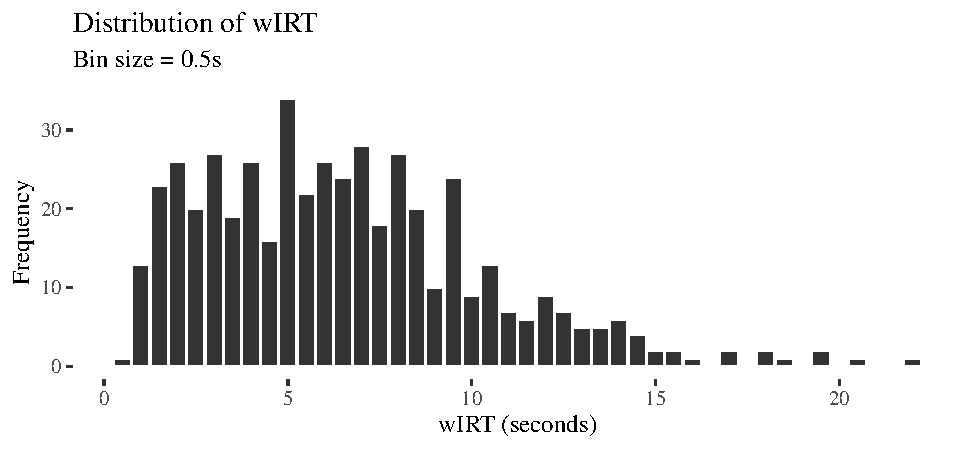
\includegraphics{4-results_files/figure-latex/wIRT-1.pdf}
\caption{\label{fig:wIRT}Distribution of IRT values for experimental sentences.}
\end{figure}

Some of the expected 3072 recordings (32 participants x 2 readings x 48 items, 16 experimental and 32 filler) could not be used due to intrusive background noise during the recording session. Additionally, data were also excluded from analysis if either of a Reading 1/Reading 2 pair was missing; 9 such incomplete pairs were excluded. Without analyzable data from both members of a pair, it is difficult to determine the extent to which the elicitation protocol was executed as intended (i.e., the extent of preview for Reading 1 vs.~Reading 2). The number of recordings per sentence type included in the analyses that follow were distributed as shown in Table \ref{tab:rvtab}; if no data had been omitted, the expected count per sentence type was 256.

\begin{table}[!h]

\caption{\label{tab:rvtab}Number of recordings analyzed, as a function of Speech Act and PP2 Status.}
\centering
\begin{tabular}{ccc}
\toprule
  & D & Q\\
\midrule
Mod & 246 & 248\\
Arg & 244 & 240\\
\bottomrule
\end{tabular}
\end{table}

For experimental items, 978 recordings were subjected to prosodic analysis, constituting 95.6\% of the utterances elicited. Because IRT is a measure arising from pairs of utterances (Reading 1 and Reading 2) rather than from single recordings, the database for response timing took in 489 data points.

\hypertarget{results-prosody}{%
\subsection{Prosodic boundary patterns}\label{results-prosody}}

This section reports the prosodic phrasings judged to be present in the recordings of experimental items, and the extent to which those patterns are influenced by the design parameters of the study (Speech Act and PP2 Status), as well as which reading (Reading 1 or Reading 2) a given recording represents. These data are reported first descriptively (i.e., in terms of occurrence frequency), and then using regression models to calculate the statistical significance of whatever patterns emerge from the data. Finally, a summary of findings and their implications for the hypothesis motivating this study is provided.

In what follows, the distribution of OBJ boundaries and PP1 boundaries are first reported, separately for the four sentence types created by the materials design (D/Q x Mod/Arg), for each of Reading 1 and Reading 2. Then, the patterns of boundaries over the two positions are considered, before moving to statistical analysis.

Note that while judgments about the potential boundary after the infinitival construction verb were collected, reports of these were sufficiently uncommon (occurring in only 8\% of recordings) to warrant their treatment as noise, and so were set aside. The break locations are indicated with a \% symbol in (39), which was previously provided in Section \ref{sita} as (38) and is repeated here for convenience.

\begin{enumerate}
\def\labelenumi{(\arabic{enumi})}
\setcounter{enumi}{38}
\tightlist
\item
  \begingroup
  \setlength{\tabcolsep}{1pt}

  \begin{tabular}{cccccccc}
    & & \footnotesize V Break & & \footnotesize OBJ Break & & \footnotesize PP1 Break & \\
    She had & wanted to set & \% & the textbooks & \% & on the top shelf & \% & into the file box. \\
    \cmidrule(r){2-2} \cmidrule(r){4-4} \cmidrule(r){6-6} \cmidrule(r){8-8} 
    & \footnotesize V Region & & \footnotesize OBJ Region & & \footnotesize PP1 Region & & PP2 Region \\
  \end{tabular}
    \endgroup
\end{enumerate}

Examination of prosodic phrasings begins with counts of the rate at which prosodic breaks were judged to be present after each of the OBJ and PP1 sentence regions: Table \ref{tab:obj} below summarizes these data, for the OBJ breaks:

\begin{table}[!h]

\caption{\label{tab:obj}Percent occurrence of OBJ boundary (frequency of occurrence in parenthesis) as a function of sentence type and Reading.}
\centering
\begin{tabular}{ccccc}
\toprule
\multicolumn{1}{c}{ } & \multicolumn{2}{c}{Reading 1} & \multicolumn{2}{c}{Reading 2} \\
\cmidrule(l{3pt}r{3pt}){2-3} \cmidrule(l{3pt}r{3pt}){4-5}
 & D & Q & D & Q\\
\midrule
Mod & 77.2\% (95) & 76.6\% (95) & 84.6\% (104) & 72.6\% (90)\\
Arg & 57.4\% (70) & 56.7\% (68) & 73.0\% (89) & 74.2\% (89)\\
\bottomrule
\end{tabular}
\end{table}

A boundary following the OBJ region was more likely overall for Mod sentences (77.8\% occurrence rate) than for Arg (65.2\%), though that contrast was more sharply drawn for Reading 1 of Arg sentences (57.2\%) than for Reading 2 (73.6\%).

Data of the same kind, now for the rates at which prosodic breaks were judged to be present after the PP1 sentence regions, are summarized in Table \ref{tab:pp1} below. Those data allow the following generalization to be drawn: Reversing the pattern for OBJ, a boundary after PP1 was judged to be present substantially less often for Mod sentences (68.0\% occurrence rate) than for Arg; for the latter type, the PP1 break was present in virtually all utterances (98.7\%). Moreover, for breaks at this position, there appeared to be no influence whatsoever of other factors in the design (Speech Act, Reading).

\begin{table}[!h]

\caption{\label{tab:pp1}Percent occurrence of PP1 boundary (frequency of occurrence in parenthesis) as a function of sentence type and Reading.}
\centering
\begin{tabular}{ccccc}
\toprule
\multicolumn{1}{c}{ } & \multicolumn{2}{c}{Reading 1} & \multicolumn{2}{c}{Reading 2} \\
\cmidrule(l{3pt}r{3pt}){2-3} \cmidrule(l{3pt}r{3pt}){4-5}
 & D & Q & D & Q\\
\midrule
Mod & 68.3\% (84) & 68.5\% (85) & 68.3\% (84) & 66.9\% (83)\\
Arg & 99.2\% (121) & 99.2\% (119) & 99.2\% (121) & 97.5\% (117)\\
\bottomrule
\end{tabular}
\end{table}

Looking at both OBJ and PP1 breaks, taken together, it is clear that the total number of breaks judged present for any sentence type within a given reading substantially exceeds the number of recorded utterances. For example, for declarative sentences with PP2 as modifier (D/Mod) produced as Reading 1, 179 construction-internal prosodic breaks occurred (95 OBJ + 84 PP1), cf.~123 recordings; thus, 45.5\% of those utterances carried both breaks. Considering all four sentences types produced as Readings 1 and Reading 2, two-break prosodic phrasing patterns were judged to have occurred in 43.0\% to 72.1\% of recordings. Appendix \ref{proApp} provides two tables and an accompanying figure spelling out the distribution of OBJ-only, PP1-only, and OBJ+PP1 break patterns. Five cases where no phrasing break was judged present were omitted in subsequent reports of prosodic patterns.

For the questions pursued in the current study, the analysis that is most germane is one considering break dominance rather than simple break occurrence. Tables \ref{tab:r1dombreaks}, \ref{tab:r2dombreaks}, and Figure \ref{fig:bdom} below therefore incorporate the informant's judgments about the relative strength of the PP1 and OBJ prosodic phrasing boundaries. PP1-dominance means that the PP1 boundary was reported to be stronger than the OBJ break boundary (or that only the PP1 boundary occurred); OBJ-dominance means the reverse; and ``Equal strength'' means that neither boundary was reported to be stronger than the other.

\begin{table}[!h]

\caption{\label{tab:r1dombreaks}Percent occurrence of boundary dominance as a function of sentence type for Reading 1.}
\centering
\begin{tabular}{>{\bfseries}lcccc}
\toprule
\multicolumn{1}{c}{ } & \multicolumn{2}{c}{Mod} & \multicolumn{2}{c}{Arg} \\
\cmidrule(l{3pt}r{3pt}){2-3} \cmidrule(l{3pt}r{3pt}){4-5}
  & D & Q & D & Q\\
\midrule
OBJ-dominant & 56.1\% (69) & 56.1\% (69) & 13.9\% (17) & 10.8\% (13)\\
Equal strength & 3.3\% (4) & 3.3\% (4) & 6.6\% (8) & 1.7\% (2)\\
PP1-dominant & 40.7\% (50) & 40.7\% (50) & 79.5\% (97) & 87.5\% (105)\\
\bottomrule
\end{tabular}
\end{table}
\begin{table}[!h]

\caption{\label{tab:r2dombreaks}Percent occurrence of boundary dominance as a function of sentence type for Reading 2.}
\centering
\begin{tabular}{>{\bfseries}lcccc}
\toprule
\multicolumn{1}{c}{ } & \multicolumn{2}{c}{Mod} & \multicolumn{2}{c}{Arg} \\
\cmidrule(l{3pt}r{3pt}){2-3} \cmidrule(l{3pt}r{3pt}){4-5}
  & D & Q & D & Q\\
\midrule
OBJ-dominant & 63.1\% (77) & 60.3\% (73) & 23.8\% (29) & 16.7\% (20)\\
Equal strength & 5.7\% (7) & 1.7\% (2) & 3.3\% (4) & 4.2\% (5)\\
PP1-dominant & 31.1\% (38) & 38.0\% (46) & 73.0\% (89) & 79.2\% (95)\\
\bottomrule
\end{tabular}
\end{table}

\begin{figure}
\centering
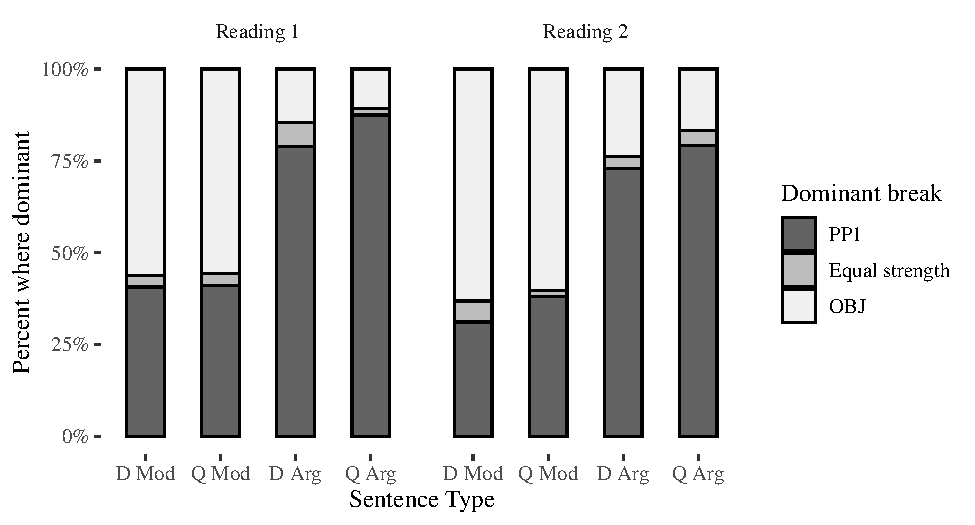
\includegraphics{4-results_files/figure-latex/bdom-1.pdf}
\caption{\label{fig:bdom}Percent break dominance occurrence as a function of sentence type and Reading.}
\end{figure}

The data here clearly show a robust effect of PP2 Status (Mod or Arg) on break dominance, and little to no impact of Reading or Speech Act (D or Q). A dominant break after PP1 is frequent for all Arg sentences, both declaratives and questions, and in both Reading 1 and Reading 2. It is less frequent for Mod sentences in both Reading 1 and Reading 2. The higher relative frequency of PP1 break dominance in Arg sentences compared to Mod sentences is expected, since it represents a syntactically motivated prosodic break in the Arg cases. For the Mod sentences, there is no syntactic motivation for the PP1 break, so it makes sense for it to be less frequent and less dominant in Mod sentences.

It is both noteworthy and puzzling that the patterns do not differ greatly across the two readings, as one would expect difficulty getting the prosody right on the first try for the difficult sentences being tested in the current study. It may be that the disambiguating preposition, \emph{into} came into view while the participant was still pronouncing an earlier portion of the sentence (due to the Eye-Voice Span, see Section \ref{look-ahead}). Since the disambiguator is a preposition and thus a function word, it can be processed very quickly, and so it's possible that even very limited lookahead allowed some readers to come to the correct parse on their first reading.

A number of mixed effects logistic regression models support the general observations above. Models predicting PP1 break, OBJ break, OBJ break dominance and PP1 break dominance are reported. All models include random intercepts for participant and item, but due to convergence errors, no random slopes for any predictors are included.

The intercept always represents the Mod sentence type, which is not expected to present any particular difficulty to the reader, since sentences with PP2 taking the role of a modifier are compatible with what is assumed to be the running parse when PP2 is encountered (i.e., PP1 has been interpreted as the goal argument of the verb, and PP2 does not disrupt that interpretation). For those models where Speech Act is included in the model, the intercept represents the declarative sentence type. In this way, the more complex sentence types are compared to the simplest one represented in the model. If Reading is included in a model, the intercept represents Reading 1.

For each analysis, a reduced model and the full model (i.e., the model containing all predictors of interest), when it converged, are reported. In each case, the reported reduced model is the simplest nested model\footnote{A simpler model nested within a more complex model is one that includes a subset of the more complex model's predictors, e.g., OBJ Dominance as a function of PP2 Status is nested within OBJ Dominance as a function of Speech Act \(\times\) PP2 Status.} that did not represent a statistically significant worse fit according to likelihood ratio tests (LRTs) than the next most complex model. This model selection process was used for each of the four analyses that follow (OBJ and PP1 boundary occurrence, OBJ and PP1 break dominance). All reported models represent statistically significant improvement over a minimal model, which was a model with only an intercept and random effects (no fixed effects). That comparison is reported for each selected reduced model, as well as the Akaike Information Criterion (AIC\footnote{AIC is a representation of the amount of information lost by using a regression model to estimate data points. It is a measure that balances both the goodness of fit of a model and the simplicity of a model, guarding against over fitting and under fitting the data involved.}) value for the selected model and the minimal model. All regression models were run using the lme4 R package (Bates, Maechler, Bolker, \& Walker (2019)).

In the full model predicting OBJ break occurrence, shown in Table \ref{tab:fullobjmod}, only the estimate for D Mod Reading 1 (the intercept) and the effect of PP2 Status show statistical significance.

\begin{table}[!h]

\caption{\label{tab:fullobjmod}Mixed effects logistic regression model predicting OBJ break occurrence (Full).}
\centering
\begin{tabular}{rcccrcccrcccrccc}
\toprule
\multicolumn{1}{c}{Outcome: OBJ break (Full)} & \multicolumn{1}{c}{Estimate} & \multicolumn{1}{c}{Std. Error} & \multicolumn{1}{c}{p}\\
\midrule
D Mod, Reading 1 (Intercept) & 0.93 & 0.59 & .11\\
Q & 0.83 & 0.74 & .26\\
Arg & -1.40 & 0.71 & < .05\\
Reading 2 & 0.56 & 0.35 & .11\\
Q:Arg & -1.03 & 1.00 & .30\\
\addlinespace
Q:Reading2 & -0.81 & 0.48 & .09\\
Arg:Reading2 & 0.29 & 0.46 & .53\\
Q:Arg:Reading2 & 0.97 & 0.65 & .13\\
\bottomrule
\end{tabular}
\end{table}

Table \ref{tab:objMod} shows a reduced model, predicting the occurrence of an OBJ break with estimates for the coefficients of the fixed effects of Reading 2, PP2 and the interaction between Reading and PP2 Status. The removal of Speech Act as a predictor revealed the Reading \(\times\) PP2 Status interaction to become a significant predictor. The model that included PP2 Status and its interaction with Reading provided a statistically significantly better fit than a minimal model (AIC\textsubscript{Minimal}=1068.0, AIC\textsubscript{Reduced}=1031.6, \(\chi^2\)(3)=42.34, p \textless{} .001).

\begin{table}[!h]

\caption{\label{tab:objMod}Mixed effects logistic regression model predicting OBJ break occurrence (Reduced).}
\centering
\begin{tabular}{rcccrcccrcccrccc}
\toprule
\multicolumn{1}{c}{Outcome: OBJ break (Reduced)} & \multicolumn{1}{c}{Estimate} & \multicolumn{1}{c}{Std. Error} & \multicolumn{1}{c}{p}\\
\midrule
Mod, Reading 1 (Intercept) & 1.39 & 0.45 & < .01\\
Reading 2 & 0.11 & 0.23 & .62\\
Arg & -1.98 & 0.50 & < .001\\
Reading2:Arg & 0.81 & 0.32 & < .05\\
\bottomrule
\end{tabular}
\end{table}

The log odds\footnote{Log odds is, in this case, the natural log of the odds ratio, so the log odds of A is log\textsubscript{e}(P(A)/P(¬A)). A log odds of 1.39 translates to an odds ratio of 4.01:1 (e\textsuperscript{1.39}=4.01) and a probability of 80\% (4.01/(1+4.01)=0.80).} of an OBJ break for Mod Reading 1 is 1.39 (std. error = 0.45, p \textless{} .01). The log odds of that break increased modestly in Reading 2 but the increase was not statistically significant. PP2 arguments reduced the log odds of an OBJ break compared to PP2 modifiers, robustly, but less so in Reading 2 than in Reading 1. As noted earlier, the OBJ break is expected to occur more often in Mod cases, because that break marks PP1 attachment as an argument of the verb.

The full model for predicting PP1 boundary occurrence showed significance only for the intercept and the effect of PP2 Status.

\begin{table}[!h]

\caption{\label{tab:fullpp1Mod}Mixed effects logistic regression model predicting PP1 break occurrence (Full).}
\centering
\begin{tabular}{rrrlrrrlrrrlrrrl}
\toprule
\multicolumn{1}{c}{Outcome: PP1 break (Full)} & \multicolumn{1}{c}{Estimate} & \multicolumn{1}{c}{Std. Error} & \multicolumn{1}{c}{p}\\
\midrule
D Mod, Reading 1 (Intercept) & 0.68 & 0.07 & < .001\\
Q & 0.01 & 0.09 & .89\\
Arg & 0.31 & 0.09 & < .001\\
Reading 2 & 0.00 & 0.04 & .99\\
Q:Arg & 0.00 & 0.13 & 0.97\\
\addlinespace
Q:Reading2 & -0.01 & 0.06 & .82\\
Arg:Reading2 & 0.00 & 0.06 & .99\\
Q:Arg:Reading2 & 0.00 & 0.08 & .97\\
\bottomrule
\end{tabular}
\end{table}

The model selection process described above found that the the best model was the one with PP2 Status as the only fixed effect, which was found to be better than a minimal model by LRT (AIC\textsubscript{Minimal}=855.59, AIC\textsubscript{Reduced}=629.60, \(\chi^2\)(1)=228, p \textless{} .001).

\begin{table}[!h]

\caption{\label{tab:pp1Mod}Mixed effects logistic regression model predicting PP1 break occurrence (Reduced).}
\centering
\begin{tabular}{rcccrcccrcccrccc}
\toprule
\multicolumn{1}{c}{Outcome: PP1 break (Reduced)} & \multicolumn{1}{c}{Estimate} & \multicolumn{1}{c}{Std. Error} & \multicolumn{1}{c}{p}\\
\midrule
Mod (Intercept) & 0.96 & 0.30 & < .01\\
Arg & 4.12 & 0.44 & < .001\\
\bottomrule
\end{tabular}
\end{table}

Sentences with argument PP2s had greatly increased log odds of a PP1 break compared to those with modifier PP2s. This is again expected, because the PP1 break is responsive to the syntactic discontinuity required for the argument attachment of PP2. That Speech Act is not a relevant predictor is evidence against a prosodic explanation of the motivating intuition for this study; we would expect both a main effect of Speech Act and definitely an interaction between Speech Act and PP2 Status, if the prosody were more (or less) different across the PP2 Status factor for interrogatives than for declaratives.

Models were also run for predicting break dominance. The full model predicting OBJ break dominance is shown in Table \ref{tab:fodom}.

\begin{table}[!h]

\caption{\label{tab:fodom}Mixed effects logistic regression model predicting OBJ break dominance (Full).}
\centering
\begin{tabular}{rcccrcccrcccrccc}
\toprule
\multicolumn{1}{c}{Outcome: OBJ-dominance (Full)} & \multicolumn{1}{c}{Estimate} & \multicolumn{1}{c}{Std. Error} & \multicolumn{1}{c}{p}\\
\midrule
D Mod, Reading 1 (Intercept) & 0.50 & 0.09 & < .001\\
Q & 0.03 & 0.12 & 0.82\\
Arg & -0.45 & 0.12 & < .001\\
Reading 2 & 0.07 & 0.05 & .22\\
Q:Arg & -0.03 & 0.17 & .86\\
\addlinespace
Q:Reading2 & -0.03 & 0.07 & .68\\
Arg:Reading2 & 0.03 & 0.07 & .71\\
Q:Arg:Reading2 & 0.00 & 0.11 & .97\\
\bottomrule
\end{tabular}
\end{table}

Table \ref{tab:odom} reports the best model for predicting OBJ break dominance. The best model was one with fixed effects for reading and PP2 Status. A likelihood ratio test (LRT) found that the selected model represented a statistically significant improvement over a minimal model (AIC\textsubscript{Minimal}=1270.5, AIC\textsubscript{Reduced}=1079.3, \(\chi^2\)(2)=219.63, p \textless{} .001). There was no statistically significant effect of Speech Act on OBJ break dominance.

\begin{table}[!h]

\caption{\label{tab:odom}Mixed effects logistic regression model predicting OBJ break dominance (Reduced).}
\centering
\begin{tabular}{rcccrcccrcccrccc}
\toprule
\multicolumn{1}{c}{Outcome: OBJ-dominance (Reduced)} & \multicolumn{1}{c}{Estimate} & \multicolumn{1}{c}{Std. Error} & \multicolumn{1}{c}{p}\\
\midrule
Mod, Reading 1 (Intercept) & -0.16 & 0.32 & .62\\
Reading 2 & 0.40 & 0.16 & < .05\\
Arg & -2.32 & 0.18 & < .001\\
\bottomrule
\end{tabular}
\end{table}

PP1 break dominance and OBJ break dominance are not entirely complementary, because it is possible for the two breaks to have equal prominence (as happens, say, when prosodic
phrasing marks out parenthetic content). Thus, models predicting PP1 dominance were also explored.

The full model predicting PP1 break dominance failed to converge, so only the reduced model is reported. Table \ref{tab:pdom} reports the best model for predicting PP1 break dominance. Unlike the model for predicting OBJ break dominance, the best model for predicting PP1 break dominance includes Speech Act as a predictor, as well as Reading, and PP2 Status.

\begin{table}[!h]

\caption{\label{tab:pdom}Mixed effects logistic regression model predicting PP1 break dominance (Reduced).}
\centering
\begin{tabular}{rcccrcccrcccrccc}
\toprule
\multicolumn{1}{c}{Outcome: PP1-dominance (Reduced)} & \multicolumn{1}{c}{Estimate} & \multicolumn{1}{c}{Std. Error} & \multicolumn{1}{c}{p}\\
\midrule
D Mod, Reading 1 (Intercept) & -0.19 & 0.33 & .57\\
Reading 2 & -0.38 & 0.15 & < .05\\
Q & 0.31 & 0.15 & < .05\\
Arg & 2.20 & 0.17 & < .001\\
\bottomrule
\end{tabular}
\end{table}

This model was better than a minimal model according to LRT (AIC\textsubscript{Minimal}=1290.4, AIC\textsubscript{Reduced}=1078.8, \(\chi^2\)(3)=217.59, p \textless{} .001). PP1 break dominance was much more likely for sentences with argument PP2s than sentences with modifier PP2s, with interrogatives having slightly increased log odds of PP1 break dominance. Log odds of PP1 break dominance were slightly less in Reading 2 than Reading 1. There were no significant interaction terms.

Because reading was a significant predictor for 3 of the 4 models reported, and there are reasons to believe that Reading 2 is more representative of the natural or intended prosody of the sentences at issue, models were also run predicting OBJ-dominance and PP1-dominance for Reading 2 data only. In both cases, the best model had the same structure: fixed effects of Speech Act and PP2 Status, with no interaction term.

\begin{table}[!h]

\caption{\label{tab:r2dom}Mixed effects logistic regression models predicting break dominance in Reading 2 (Reduced).}
\centering
\begin{tabular}{rcccrcccrcccrcccrcccrcccrccc}
\toprule
\multicolumn{1}{c}{ } & \multicolumn{3}{c}{Outcome: OBJ Dominance} & \multicolumn{3}{c}{Outcome: PP1 Dominance} \\
\cmidrule(l{3pt}r{3pt}){2-4} \cmidrule(l{3pt}r{3pt}){5-7}
\multicolumn{1}{c}{(Reading 2 only)} & \multicolumn{1}{c}{Estimate} & \multicolumn{1}{c}{Std. Err} & \multicolumn{1}{c}{p} & \multicolumn{1}{c}{Estimate} & \multicolumn{1}{c}{Std. Err} & \multicolumn{1}{c}{p}\\
\midrule
D Mod (Intercept) & 0.66 & 0.24 & < .01 & -0.97 & 0.27 & < .001\\
Q & -0.30 & 0.22 & .16 & 0.35 & 0.22 & .10\\
Arg & -2.07 & 0.24 & < .001 & 2.15 & 0.24 & < .001\\
\bottomrule
\end{tabular}
\end{table}

For both OBJ-dominance and PP1-dominance, the main effect of Speech Act failed to reach significance, but its inclusion marginally improves the fit of each model. Even when limited to only Reading 2 data, Speech Act does not interact with PP2 Status, which is again supportive of a non-prosodic explanation for the motivating intuition. That there is a robust effect of PP2 Status is reassuring evidence that prosody is indeed sensitive to syntax, and that the study's material design has driven both the intended initial parse and re-analysis for the Arg sentence-types, where PP2 takes the role of goal argument to the construction verb.

\hypertarget{irt}{%
\subsection{Inter-reading time}\label{irt}}

Inter-reading time\footnote{Since IRT is a measure across pairs of recordings (Reading 1/Reading 2), the number of data analyzed in this section are half as many as those in the prosody analyses.} is the time elapsing between the completion of Reading 1 and before the start Reading 2 phonation. The details of how this was measured and defined can be found in Section \ref{method-irt}. Possibly, IRT can provide an estimate of how much difficulty the reader has in processing a given sentence. If a reader spends more time studying a sentence prior to reading it aloud a second time, the IRT is longer; it is thus a possible indicator of processing difficulty.

\begin{figure}
\centering
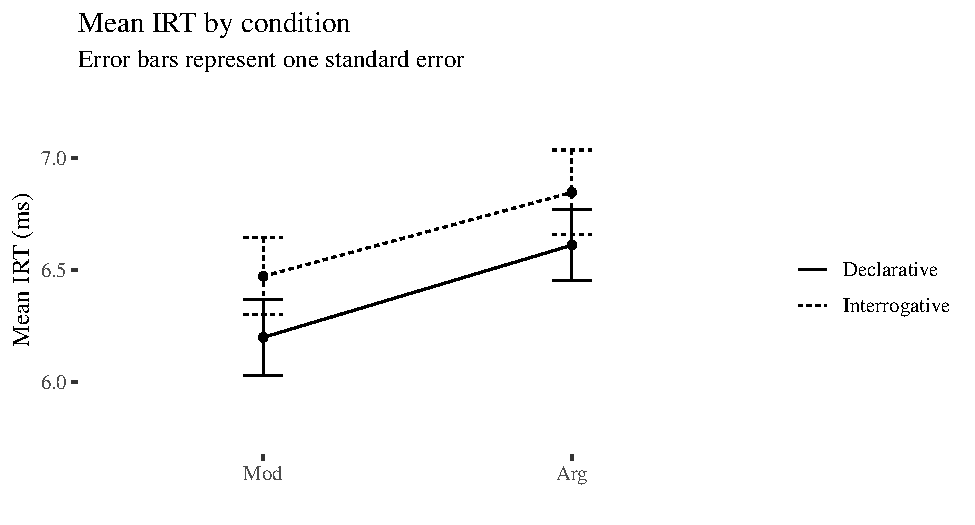
\includegraphics{4-results_files/figure-latex/interactionplot-1.pdf}
\caption{\label{fig:interactionplot}Mean IRT as a function of sentence type.}
\end{figure}

Figure \ref{fig:interactionplot} graphs mean IRT values as a function of sentence type. The two slopes diverge minimally. PP2 Status has a statistically significant effect on IRT: sentences with argument PP2s having substantially longer IRTs (6.73s) on average than those with modifier PP2s (6.34s). The effect of Speech Act was not statistically significant, though interrogatives attracted longer (6.66s) IRTs than declaratives (6.40s), and including Speech Act as a predictor of IRT improved the predictive power of the model. This is discussed in more detail below.

Regression models support the observations above. All models discussed include random intercepts for participant and item. Models with random slopes did not converge, and so random slopes were not included.

The full model for predicting IRT included fixed effects of Speech Act and PP2 Status and their interaction. This model is shown in Table \ref{tab:hyp}.

\begin{table}[!h]

\caption{\label{tab:hyp}Linear mixed effects regression model predicting IRT by sentence type with interaction term (Full).}
\centering
\begin{tabular}{rcccrcccrcccrccc}
\toprule
IRT Full Model & Estimate & Std. Error & p\\
\midrule
D Mod (Intercept) & 6.32 & 0.59 & < .001\\
Q & 0.29 & 0.30 & .34\\
Arg & 0.42 & 0.30 & .17\\
Q:Arg & 0.08 & 0.43 & .85\\
\bottomrule
\end{tabular}
\end{table}

Of the nested models (those with subsets of the full model), the best model according to likelihood ratio testing (LRT) was the one with only the fixed effect of PP2 Status, shown in Table \ref{tab:redirt}. The improvement of fit of the reduced model over a minimal model with only an intercept and random effects was statistically significant (AIC\textsubscript{Reduced}=2346.2, AIC\textsubscript{Minimal}=2348.7, \(\chi^2\)(1)=4.51, p \textless{} .05), indicating a robust main effect of PP2 Status on IRT.

\begin{table}[!h]

\caption{\label{tab:redirt}Linear mixed effects regression model predicting IRT by sentence type (Reduced).}
\centering
\begin{tabular}{rcccrcccrcccrccc}
\toprule
IRT Reduced Model & Estimate & Std. Error & p\\
\midrule
Mod (Intercept) & 6.47 & 0.58 & < .001\\
Arg & 0.46 & 0.21 & < .05\\
\bottomrule
\end{tabular}
\end{table}

These results are not supportive of \emph{Hypothesis 3} formalized in Section \ref{pred}, as statistical significance was expected for the interaction of Speech Act with PP2 Status under the assumption that interrogative context ameliorates processing difficulty for PP-attachment garden paths, vs.~declarative context for the same construction.

\hypertarget{discussion-of-planned-analyses}{%
\subsection{Discussion of planned analyses}\label{discussion-of-planned-analyses}}

Throughout the analysis of prosodic phrasing patterns, PP2 Status was the most robust predictor of OBJ and PP1 boundary occurrence and their relative strengths. The PP1 break was more frequent and more frequently dominant for sentences with a PP2 that was an argument than those with a PP2 that could be a modifier; conversely, the OBJ break was more frequent and more frequently dominant for sentences with a PP2 that was interpretable as a modifier than those with a PP2 that was an argument.

Returning to the predictions discussed in Section \ref{pred}, recall the contrast made there between syntactically motivated prosodic breaks and other breaks or pauses. The Arg and Mod sentences differ with regard to where such breaks are expected to fall. These expectations are shown in (40) and (41) (originally formulated in Chapter 1 and repeated here for convenience), where ``\(\|\)'' represents a syntactically motivated prosodic break.

\singlespacing

\begin{enumerate}
\def\labelenumi{(\arabic{enumi})}
\setcounter{enumi}{39}
\tightlist
\item
  \textbf{Mod pattern}
  \begingroup
  \setlength{\tabcolsep}{2pt}

  \begin{tabular}{ccccccc}
    \dots & stick & the letter & $\|$ & in the mailbox &  & of the proper stack \\
    & & \footnotesize Direct object & & \footnotesize PP1 & & \footnotesize vice president. \\
  \end{tabular}
    \endgroup
\item
  \textbf{Arg pattern}
  \begingroup
  \setlength{\tabcolsep}{2pt}

  \begin{tabular}{ccccccc}
    \dots & stick & the letter & & in the mailbox & $\|$ & onto the proper stack. \\
    & & \footnotesize Direct object & & \footnotesize PP1 & & \footnotesize PP2 \\
  \end{tabular}
    \endgroup
\end{enumerate}

\doublespacing

Consider again \emph{Hypotheses 1} and \emph{2} from Section \ref{pred}, repeated below.

\begin{enumerate}
\def\labelenumi{(\arabic{enumi})}
\setcounter{enumi}{41}
\tightlist
\item
  \emph{Hypothesis 1} (Prosodic Errors)\linebreak\nopagebreak
  A first reading of a sentence where PP2 is a goal argument (Arg) will be more likely to exhibit less natural prosody (e.g., more hesitation at and within the PP2 region) than either:

  \begin{enumerate}
  \def\labelenumii{\alph{enumii}.}
  \tightlist
  \item
    A first reading of a sentence where PP2 is a modifier (Mod)
  \item
    A second reading of a sentence where PP2 is a goal argument (Arg)
  \end{enumerate}
\end{enumerate}

While the present study did not specifically attempt to assess whether a given reading represents more or less natural prosody for these constructions, given that there is a difference between readings, it seems most likely that Reading 2 is the more natural of the two since it represents a considered reading, rather than a hurried one without as much preview. \emph{Hypotheses 1} is fully supported only on the assumption that this is so. The robust effect of PP2 Status throughout all of the regression models of prosodic phrasing, however, suggests that at least the (a) portion of the both \emph{Hypothesis 1} above and \emph{Hypothesis 2} below are supported, if reading is disregarded. That Reading 2 is a significant predictor of both OBJ-dominance and PP1-dominance supports the (b) portions of these two hypotheses.

\begin{enumerate}
\def\labelenumi{(\arabic{enumi})}
\setcounter{enumi}{42}
\tightlist
\item
  \emph{Hypothesis 2} (Prosody/Syntax Mismatch)\linebreak\nopagebreak
  A first reading of a sentence where PP2 is a goal argument (Arg) will more often be produced with prosodic structure that represents an implausible or ungrammatical parse of the string (i.e., PP2 incorrectly attached as a modifier) than either:

  \begin{enumerate}
  \def\labelenumii{\alph{enumii}.}
  \tightlist
  \item
    A first reading of a sentence where PP2 is a modifier (Mod)
  \item
    A second reading of a sentence where PP2 is a goal argument (Arg)
  \end{enumerate}
\end{enumerate}

\emph{Hypothesis 2} is fairly well supported: the (a) portion by the significant effect of PP2 Status on OBJ-dominant and PP1-dominant pronunciations, and the (b) portion by the significance of Reading on the same. That said, the results do not represent a perfect correlation. Setting Reading 1 aside, Arg sentences (whether D or Q) were found to have the Arg-optimal pronunciation in almost 80\% of recordings (PP1-dominant pronunciations), leaving some 22\% of pronunciations as prosody/syntax mismatches (OBJ-dominant). For Mod sentences (whether Q or D), the picture is similar, but with a weaker contrast: prosodic coding identifies the Mod-optimal pronunciation in some 64\% of recordings (OBJ-dominant). That leaves nearly one-third of pronunciations as prosody/syntax mismatches (PP1-dominant). Given the assumption that for Reading 2 a participant should already know the structure of the sentence and its interpretation, it is not entirely clear why some Reading 2 pronunciations still do not represent to the expected pattern.

It could be that for some participants and some sentences the intended interpretation of the sentence is never grasped because the level of complexity was simply too high, or for some other reason. It might also be that while the participant arrived at the intended syntax, it was too difficult to devise or produce the prosodic phrasing that corresponds with that syntax. Finally, it is possible that the prosodic coding was imperfect, given the difficulty of evaluating prosodic phenomena, even for ToBI experts and other highly trained linguists. Most likely, all three of these possibilities are at play, and some portion of the cases of prosody/syntax mismatch can be attributed to each.

Returning to the predictions made in the first chapter, and indeed the intuition that motivated this line of research, it should be noted that \emph{Hypothesis 3} (repeated here for convenience) as originally formalized is not supported by the facts.

\begin{enumerate}
\def\labelenumi{(\arabic{enumi})}
\setcounter{enumi}{43}
\tightlist
\item
  \emph{Hypothesis 3}
  The inter-reading time (IRT) will be longer for Arg sentences that are declarative than for:

  \begin{enumerate}
  \def\labelenumii{\alph{enumii}.}
  \tightlist
  \item
    Arg sentences that are interrogative
  \item
    Mod sentence that are interrogative or declarative
  \end{enumerate}
\end{enumerate}

The prediction made by this hypothesis is essentially that IRT would show an effect of the interaction between PP2 Status and Speech Act, but no such significance was detected. It is possible that this is because IRT is not the proper measure for processing difficulty, but to make that claim one would have to explain why it nonetheless shows a robust effect of Arg PP2 Status (i.e., garden-path sentences exhibit longer IRTs than non-garden-path sentences). It seems more likely that IRT is a useful measure of processing difficulty, but that for some other reason, the intuition that the declarative instances of the Arg sentences are harder to process than the interrogative versions is not reflected in IRT.

\hypertarget{qslow}{%
\subsection{An ancillary planned analysis, the processing cost of interrogativity}\label{qslow}}

It is worth noting that the mean IRT for interrogative versions (6.7s) of the experimental sentences in the reported study was longer than for the declaratives (6.4s). While this finding was not statistically significant, Peckenpaugh (2016) found that whole-sentence silent reading times for interrogatives were longer than for declaratives; and Mehler (1963) provided a very early report of the processing cost of interrogativity: a so-called kernel sentence, i.e., a simple declarative, was easier to recall verbatim than were a number of sentences that he considered to be syntactic transformations of that kernel sentence (K): negative (N), polar question (Q), passive (P), and combinations thereof: NQ, NP, QP and NPQ. Mehler found that accurate recall was more frequent for K sentences (300/460, 65.2\%) than for the other sentences types, with interrogatives (210/460, 45.7\%) being recalled accurately at a lower rate than the two other individual transformations (234/460, 50.9\% for N; 243/460, 52.8\% for P).

To further investigate the effect that interrogativity appears to have on processing, the filler sentences in this study were designed in two versions, interrogative (Q) and declarative (D), so as to provide a diagnostic of the interrogative effect on IRT outside the construction of interest. A linear mixed effects regression model predicting IRT for filler items by Speech Act with random intercepts for participant and item found that IRT is increased by 0.4s for interrogatives (std. error = 0.2; p \textless{} .05); declaratives had a mean IRT of 6.2s, while interrogatives had a mean IRT of 6.6s. Half of the fillers had a sequence of two PPs at the end of the sentence to mirror the experimental items: a model predicting IRT by the presence of those PPs found minimal effect on IRT (\(\beta\)=0.01, std. error = 0.22, p = .96). This indicates that the presence of a string of PPs does not independently affect the apparent processing cost of interrogativity.

Interrogative status itself appears to increase the time needed for participants to feel they have satisfactorily studied a sentence in order to read it aloud correctly. This is consistent with the Mehler (1963) and Peckenpaugh (2016) findings that interrogatives are in some way more complicated or difficult than declaratives, and is an interesting finding, although not clearly related to the primary research question behind this study.

\hypertarget{exploratory-analyses}{%
\section{Exploratory analyses}\label{exploratory-analyses}}

This section presents two exploratory analyses that were conducted in an effort to explain some of the surprising findings just reported.

One looks at protocol adherence, to investigate whether the lack of effect of Reading on prosodic boundary occurrence can be attributed to look-ahead. The results of that analysis suggest that look-ahead was most likely not at play.

The second exploratory analysis looks at the identity of PP2-heads and finds that \emph{of}-headed PP2s (which are categorized as Mod PP2 Status) corresponded to shorter IRTs than did \emph{from}-headed PP2s (despite \emph{from}-headed PP2s also being categorized as Mod).

\hypertarget{r1del}{%
\subsection{On Reading 1 delay}\label{r1del}}

Reading 1 (R1) delay is the amount of time between the initial display of a sentence and the start of phonation. Participants' median R1 delay ranged from 0.6s to 1.6s with a standard deviation of 0.25s. The distribution of R1 delay was notably different than that of R2 delay, as shown in Figure \ref{fig:delayComparison}, which indicates that participants were adhering to the protocol at least most of the time.

\begin{figure}
\centering
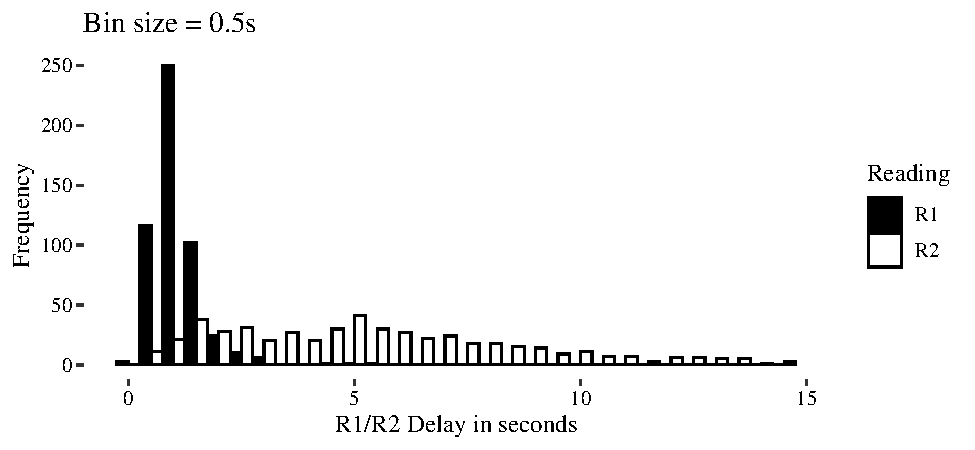
\includegraphics{4-results_files/figure-latex/delayComparison-1.pdf}
\caption{\label{fig:delayComparison}Distributions of R1 delay and R2 delay}
\end{figure}

As a way of analyzing the protocol, and the extent to which participants performed as expected, participants were categorized based on their median R1 delay. In what follows, a \emph{fast} median R1 delay was less than or equal to 0.9s, and a \emph{slow} one was longer than 1.05s, resulting in 12 participants per category. Ten participants had R1 delays between those values and were set aside. The calculations for categorizing participants were done over Reading 1 of experimental items (n = 489). Note that while R1 delay category (i.e., \emph{fast} or \emph{slow}) is a property of R1 delay, data for both readings is nonetheless explored within these categories.

\begin{figure}
\centering
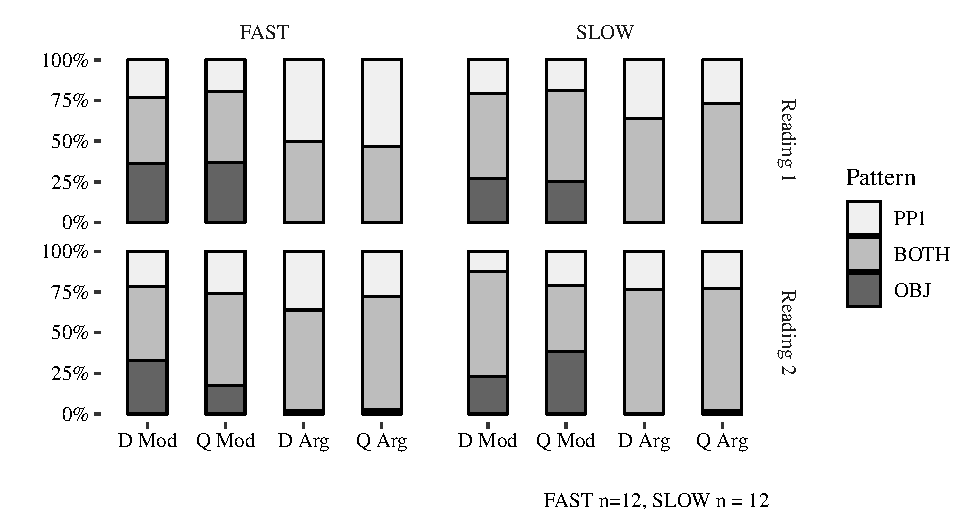
\includegraphics{4-results_files/figure-latex/facet-1.pdf}
\caption{\label{fig:facet}Plot of pattern proportions as a function of sentence type.}
\end{figure}

In cases where median R1 delay was short, readers were more likely to produce only one break (PP1 or OBJ) than if R1 delay was longer. A possible explanation is that for recordings in the \emph{slow} category, readers were more prone to hesitation in general, or perhaps, contrary to instructions, were using both the delay time as well as extra time created via hesitation to look ahead. The significant effect of PP2 Status for the \emph{slow} category in Reading 2 could be due to the reader not fully understanding the Arg sentences prior to Reading 2, thus increasing their likelihood of hesitation; i.e., where the fast category represents confident readers, the \emph{slow} category represents less confident readers. As a result of the reader's increased difficulty in Reading 1 for the recordings in the \emph{slow} category, the effect of processing difficulty is not limited to Reading 1 but in fact spills over into Reading 2. The \emph{slow} category represents readers who are never able to fully comprehend the sentence, and thus hesitate more frequently.

Mixed effects logistic regression models found no significant effect of R1 Delay Category for PP1 break dominance or OBJ break dominance. So, ultimately, variation in R1 delay does not seem to be of concern.

\hypertarget{pp2h}{%
\subsection{On PP2 heads}\label{pp2h}}

As mentioned in the items description (Section \ref{exps}), half of the items used \emph{of} for the head of PP2 in the Mod cases, while half used \emph{from.} In the Arg condition, half used \emph{into} and half used \emph{onto} to head PP2. An analysis that attempts to predict IRT by the PP2 head (e.g., \emph{into} vs.~\emph{from}) found that while \emph{into} and \emph{onto} do not behave differently from each other, \emph{of} and \emph{from} do. Starting from a maximally complex model that included the lexical identity of the matrix verb, the construction verb, the head of PP1, and the head of PP2, as well as Speech Act and PP2 Status, the model that best predicted IRT was one that is essentially the same as the reduced model just reported (i.e., with Speech Act and PP2 Status as predictors), except that it substitutes the lexical identity of the PP2 head for PP2 Status, with \emph{into} and \emph{onto} collapsed into one level used as the reference level (intercept).

\begin{table}[!h]

\caption{\label{tab:pp2hd}Linear mixed effects regression model predicting IRT by Speech Act and PP2 head.}
\centering
\begin{tabular}{rcccrcccrcccrccc}
\toprule
PP2 head model & Estimate & Std. Error & p\\
\midrule
D \em{into/onto} (Intercept) & 6.76 & 0.58 & < .001\\
Q & 0.32 & 0.21 & .13\\
\em{from} & -0.08 & 0.27 & .77\\
\em{of} & -0.84 & 0.27 & < .01\\
\bottomrule
\end{tabular}
\end{table}

Sentences where PP2 was headed by \emph{of} typically had IRTs that were 0.84s faster than sentences where PP2 was headed by \emph{into}/\emph{onto}; when the PP2 head was \emph{from}, IRT was only 0.08s faster than for \emph{into}/\emph{onto}, a difference that is not statistically significant (p \textgreater{} .50).

It is clear from the above that the sentences containing argument PP2s tested here (ones headed by \emph{into}/\emph{onto}) result in longer IRT measures than those containing Mod PP2s (\(\beta\) = 0.46, p \textless{} .05), but Speech Act and the interaction between the two factors are not a significant predictors of IRT (see Section \ref{irt}). It then must be said that IRT does not represent a behavioral reflex of the intuition that interrogativity makes difficult to process PP2-attachment ambiguities easier.

What might explain the difference in PP2 heads' effect on IRT? For one, the \emph{of}-headed PPs are marked by \emph{of} as the possessors of the noun in the immediately preceding PP1; e.g., \emph{on the roof rack of the minivan} could be re-cast as \emph{on the minivan's roof rack}. In contrast, the \emph{from}-headed PP2s are all locatives, and in that sense are similar to cases with \emph{into/onto}. It is just that the \emph{from} phrases are not the kind of locatives that can function as the goal arguments demanded by the construction verbs used in the study. That is, even if these were to be used in some circumstances as directional rather than purely locative prepositions, they would function as sources rather than goals, e.g., \emph{he moved the cows from the pasture to the barn}.

There might also be a simpler (and less interesting) explanation: because \emph{of} is only two characters long, whereas \emph{from} and \emph{into}/\emph{onto} are all four characters, participants may have recognized a pattern. For instance, they may have deduced that a two-character PP2 head meant the sentence did not have the difficult properties of some of the sentences with four-character PP2 heads (most notably the \emph{into}/\emph{onto} cases), which would have eliminated some of the needed study time.

\hypertarget{summary}{%
\section{Summary}\label{summary}}

PP2 Status is a significant predictor of prosodic boundary occurrence, prosodic boundary dominance, and inter-reading time (IRT). This is reassuring with regard to the design of the study, and supportive of the well established finding that syntax can influence prosody. It is also supportive of the claim made here, that IRT is a useful diagnostic of sentence complexity and processing difficulty.

Speech Act was not a significant predictor of prosodic phrasing, with the exception of PP1-dominance. That it was not a significant predictor of boundary occurrence or of OBJ-dominance is not supportive of the hypotheses about its apparent ameliorating effect on difficult to process sentences made prior to this study. That it was a significant predictor in one analysis leaves open the possibility that those hypotheses are not entirely false.

Speech Act was not a significant predictor of IRT for the experimental items, but did appear to be a reliable predictor of longer IRTs in the filler items (which lacked the garden-path properties of the Arg experimental items), relative to otherwise identical declarative sentences.

Ultimately, the apparent ameliorating effect of interrogativity on otherwise difficult to process declarative sentences with PP-attachment ambiguities does not appear to have a behavioral correlate that has been detected in this study. No significant interaction between Speech Act and PP2 Status was found for any of the analyses conducted.

\clearpage

\hypertarget{general-discussion}{%
\chapter{General discussion}\label{general-discussion}}

\setlength\parindent{24pt}\setlength{\parskip}{0.0pt plus 1.0pt}

This chapter will review the questions motivating the experimental study just reported and discuss the extent to which those questions are answered, or not. It will then go on to develop further questions, and propose further studies to explore those new questions and the ones left unanswered here. Finally, it will summarize the findings and the current standing of this area of research.

Recall that the primary motivation for this study was the possibility that PP-attachment garden paths are easier to understand for speakers of American English when presented in the interrogative, as opposed to the declarative. In Section \ref{obs}, a distinction was made between the intuition first outlined in Peckenpaugh (2016) and the current hypothesis. For terminological clarity, recall the definitions originally given in \ref{obs}:

\begin{enumerate}
\def\labelenumi{(\arabic{enumi})}
\setcounter{enumi}{44}
\item
  \emph{The 2016 Intuition:} Certain pragmatically disambiguated prepositional phrase (PP) attachment ambiguities which are difficult to parse in the declarative are less difficult to parse when presented as yes-no interrogatives (e.g., \emph{Jed had crammed the newspapers under the sofa in the trashcan}, vs.~\emph{Had Jed crammed the newspapers under the sofa in the trashcan?})
\item
  \emph{The Current Hypothesis:} The 2016 Intuition may be extensible to PP attachment ambiguities that are syntactically disambiguated in addition to those that are pragmatically disambiguated (e.g., \emph{He had planned to cram the paperwork in the drawer into his briefcase}, vs.~\emph{Had he planned to cram the paperwork in the drawer into his briefcase?}).
\end{enumerate}

The goal of this study was to establish whether there is evidence for (46), and to explore the implications of those findings for possible explanations of (45).

\hypertarget{behavioral-correlate-for-the-2016-intuition-and-the-current-hypothesis}{%
\section{Behavioral correlate for the 2016 intuition and the current hypothesis?}\label{behavioral-correlate-for-the-2016-intuition-and-the-current-hypothesis}}

Ultimately, no evidence has been found to support the Current Hypothesis, that the 2016 Intuition can be extended to syntactically disambiguated sentences. Mixed-effect regression analyses were not able to detect statistical significance for the interaction between Speech Act and PP2 Status. This does not, of course, negate the 2016 Intuition; it simply means that we have not yet found a behavior that can be said with certainty to correspond to that intuition. Future research should pursue the possibility that IRT (Inter-reading Time) is not the ideal measure for detecting any behavioral correlate of the processing difference for PP-attachment garden paths between interrogatives and declaratives.

\hypertarget{on-possible-explanations-for-the-intuition}{%
\section{On possible explanations for the intuition}\label{on-possible-explanations-for-the-intuition}}

This section considers the evidence for and against some of the possible explanations for the 2016 Intuition reported in Peckenpaugh (2016). While evidence of a behavioral correlate has not been found, it is nonetheless interesting to consider the source of the intuition itself.

\hypertarget{prep}{%
\subsection{A prosodic account}\label{prep}}

The prosodic phrasings produced by participants in this study varied systematically by PP2 Status (Arg vs.~Mod, where Arg is the garden path case). This is an interesting finding in and of itself, adding to the growing literature that shows a link between syntactic structure and prosodic phrasing. A possible explanation for the intuitive effect of interrogativity on parsing garden paths is provided in the work by Bader (1998). Bader demonstrates that it is easier to recover from a failed parse that ``behave{[}s{]} alike prosodically'' to a given failed parse, because the reanalysis does not require prosodic reconstruction and only the syntax needs to be repaired. In the case of the 2016 Intuition, e prosodically similar across the Arg vs.~Mod PP2 Status in the interrogative than in the declarative, the intuited reduction in difficulty of reanalysis would naturally follow. This is not relevant, of course, unless the 2016 Intuition is eventually confirmed, despite the inconclusive results of Peckenpaugh (2016).

The findings of the current study show that there is no one-to-one mapping between prosodic structure and the four sentence types tested in this study (Q Arg, D Arg, Q Mod, D Mod). Rather, for each Sentence Type, gradient differences in occurrence of each pattern were observed. Recall that a break after the object region is referred to as the object break (OBJ), and one after the PP1 region is referred to as the PP1 break (PP1).

\begin{enumerate}
\def\labelenumi{(\arabic{enumi})}
\setcounter{enumi}{46}
\tightlist
\item
  \begingroup
  \setlength{\tabcolsep}{1pt}

  \begin{tabular}{cccccccc}
    & & \footnotesize V Break & & \footnotesize OBJ Break & & \footnotesize PP1 Break & \\
    She had & wanted to set & \% & the textbooks & \% & on the top shelf & \% & into the file box. \\
    \cmidrule(r){2-2} \cmidrule(r){4-4} \cmidrule(r){6-6} \cmidrule(r){8-8} 
    & \footnotesize V Region & & \footnotesize OBJ Region & & \footnotesize PP1 Region & & PP2 Region \\
  \end{tabular}
    \endgroup
\end{enumerate}

If the prosodic structures shown in (48), (49), (50) and (51) (see below) are assumed to be phonologically ideal, then an explanation for the 2016 intuition (and by extension, the same explanation for syntactically disambiguated cases) presents itself. The symbol ``\%'' is being used in these examples to represent a prominent prosodic break.

\begin{enumerate}
\def\labelenumi{(\arabic{enumi})}
\setcounter{enumi}{47}
\tightlist
\item
  \emph{D Arg}: He had crammed {[}\textsubscript{OBJ} the newspapers{]} {[}\textsubscript{PP1} under the sofa{]} \% {[}\textsubscript{PP2} into the trashcan{]}.
\item
  \emph{D Mod}: He had crammed {[}\textsubscript{OBJ} the newspapers{]} \% {[}\textsubscript{PP1} under the sofa {[}\textsubscript{PP2} in the guestroom{]}{]}.
\end{enumerate}

The two declarative versions differ from each other in that the Arg case is ideally pronounced with a prominent break after PP1 (\emph{under the sofa}) to mark the goal argument attachment of PP2; whereas the Mod case does not require that break in the ideal pronunciation (though it may sometimes occur for length reasons). That is, the PP1 break in the D Arg case differentiates the two syntactic structures and signals the attachment site of PP2 as higher than PP2.

For the interrogatives, though, this contrast is possibly obscured by the need to apply a rising prosodic contour over the final nuclear accent in the sentence: i.e., the noun within PP2 in both Arg and Mod. The effect on melody that the speaker's anticipation of a tonal change (due to final-rise question melody) has might sound very similar to a prosodic break. The symbol ``\(\Uparrow\)'' in (50) and (51) indicates the start of the rising contour, and ``\(\Rightarrow\)'' the point in the string where preparation might begin.

\begin{enumerate}
\def\labelenumi{(\arabic{enumi})}
\setcounter{enumi}{49}
\tightlist
\item
  \emph{Q Arg}: Had he crammed {[}\textsubscript{OBJ} the newspapers{]} {[}\textsubscript{PP1} under the sofa{]} \%\(\Rightarrow\) {[}\textsubscript{PP2} into the \(\Uparrow\) trashcan{]}?
\item
  \emph{Q Mod}: Had he crammed {[}\textsubscript{OBJ} the newspapers{]} {[}\textsubscript{PP1} under the sofa \(\Rightarrow\) {[}\textsubscript{PP2} in the \(\Uparrow\) guestroom{]}{]}?
\end{enumerate}

The critical issue here is that in (51), the absence of a syntactically-motivated break before PP2 might be obscured by the hesitation necessitated by preparing to start the final-rising contour of the question two words later. It is not impossible that the need to make the articulatory preparation necessary to execute a rising contour could result in a hesitation or pause at the preceding syntactic juncture most welcoming to it, the PP1 break position. While in (51) PP2 is a sub-constituent of PP1, and so the final phrase of the VP is actually PP1, the final nuclear accent in (51) still falls on the NP within PP2. Thus the final high rise is anchored to the same phrase in both interrogative versions (Arg and Mod), and is unable to disambiguate any confusion about the presence or absence of a true prosodic boundary before PP2.

If the PP1 dominance is treated as the main indicator of the prosodic structure, then the smaller difference across PP2 Status for interrogatives (0.2\%) than for declaratives (12.2\%) does, though perhaps weakly, leave open the door for the Bader (1998) style explanation of the hunch that interrogative PP-attachment garden paths are easier to comprehend than declarative ones. Ultimately, though, logistic regression models showed no significant effect of the interaction between Speech Act and PP2 Status (no bias toward higher Arg PP2 attachment in interrogatives than declaratives), so it is safest to assume that the numerical difference is just noise, and that the explanation for the intuition is not prosodic.

\hypertarget{hesi}{%
\subsection{Hesitations vs.~prosodic breaks}\label{hesi}}

An issue with the findings of this study is the difficulty in differentiating between linguistically-motivated prosodic breaks and hesitations. As shown by the reliability data reported in Section \ref{rel}, linguistically trained judges will not necessarily be able to agree where breaks fall and which breaks are stronger, perhaps in part because of the difficulty in differentiating between prosodic breaks and hesitations.

It can be difficult to capture a prosodic break in physical terms (see, e.g., Ladd (2008)), and there is no guarantee that examining the wave forms instrumentally would fare any better than judges' intuitions in distinguishing between hesitation and true prosodic boundaries. That said, it may be possible to find means to distinguish the two sorts of breaks: for instance, it might be that boundary tones or segmental lengthening are typically not part of a hesitation break, but are a part of a prosodic break, for example.

It is possible that the results of the current study were impacted by issues with prosodic coding related to this difficulty in distinguishing between prosodic phenomena. Table \ref{tab:combobr} shows the distribution of the possible break patterns (PP2 break only, OBJ break only, or both breaks, with the negligible number of cases of neither break omitted) as a function of sentence type for Reading 2 only.

\begin{table}[!h]

\caption{\label{tab:combobr}Percent occurence of boundaries (frequency in parenthesis) in Reading 2 as a function of sentence type.}
\centering
\begin{tabular}{>{\bfseries}lcccc}
\toprule
\multicolumn{1}{c}{ } & \multicolumn{2}{c}{Mod} & \multicolumn{2}{c}{Arg} \\
\cmidrule(l{3pt}r{3pt}){2-3} \cmidrule(l{3pt}r{3pt}){4-5}
  & D & Q & D & Q\\
\midrule
OBJ-dominant & 54.1\% (66) & 43.0\% (52) & 72.1\% (88) & 71.7\% (86)\\
Equal strength & 31.1\% (38) & 31.4\% (38) & 0.8\% (1) & 2.5\% (3)\\
PP1-dominant & 14.8\% (18) & 25.6\% (31) & 27.0\% (33) & 25.8\% (31)\\
\bottomrule
\end{tabular}
\end{table}

While there is a larger drop in the number of utterances with both breaks from Arg to Mod for questions (71.7\% - 43.0\%) than for declaratives (72.1\% - 54.1\%), the opposite is true for the pattern with a PP1 break by itself (25.8\% - 25.6\%, vs.~27.0\% - 14.8\%). There is an argument to be made that the OBJ break in the Arg versions is not a true prosodic break but merely a hesitation due to a moment of confusion or for length reasons. Note that the phrase lengths within the sentence materials for the current study were similar across items and may have influenced the optimal prosodic phrasing and therefore the presence or absence of some of the breaks discussed here. For explanations of length effects on syntactic parsing see, e.g., Clifton, Carlson, \& Frazier (2006), Webman-Shafran \& Fodor (2016), and Dinçtopal Deniz \& Fodor (2017).

In \ref{erp} I propose that an event-related potential (ERP) paradigm might hold the key for distinguishing between true prosodic boundaries and hesitation.

\hypertarget{a-processing-illusion}{%
\subsection{A processing illusion}\label{a-processing-illusion}}

If the above explanation of a null result proves not to be viable in subsequent study, a possibility to consider is that the intuition itself is illusory in nature, i.e., it is not the case that interrogative PP-attachment garden paths (either pragmatically or syntactically disambiguated) are easier to parse than declarative ones, but only appear to be so because the added complexity of the interrogative version is distracting the reader with a different sort of difficulty. That is, it may be that readers are being distracted by the processing cost of interrogativity, and thereby are less sensitive to the cost of reanalysis. While the parser is struggling with two additive increases to complexity as compared to the D Mod sentences (i.e., Arg PP2 Status and interrogative status), the reader is aware only of the more immediately obvious difference, that of interrogativity, and fails to notice the structural reanalysis that the parser is undertaking.

\hypertarget{sem}{%
\subsection{A semantic/pragmatic explanation}\label{sem}}

There are substantial pragmatic and semantic differences between the interrogative and declarative versions of the Double PP construction. It is worth considering the possibility that those differences might have been what led to the 2016 Intuition. Specifically, as discussed in Section \ref{intg}, to the extent that questions more often recieve narrow focus than do declaratives, it could be that the presupposition of most of the question reduces the semantic processing load for the listener or reader. Thus, extra processing capacity is freed up to deal with the garden-path.

A possible method for exploring this potential explanation would be to test declarative sentences with marked narrow focus as in (52) (where capital letters indicate verbal emphasis).

\begin{enumerate}
\def\labelenumi{(\arabic{enumi})}
\setcounter{enumi}{51}
\tightlist
\item
  He had crammed the NEWSPAPERS under the sofa in the guestroom.
\end{enumerate}

It would be predicted that, if narrow focus where the ameliorating factor, a declarative sentence such as (52) should be likewise ameliorated, just as in the interrogative cases. However, there are several issues that would need to be dealt with in order for such an experiment to be decisive. For instance, narrow focus is less easily made pragmatically appropriate in declaratives than in interrogatives, so some clarifying context would be necessary to create felicitous declarative materials.

\hypertarget{confound}{%
\section{Conclusions and future directions}\label{confound}}

In this section, I will discuss some of the potential issues raised by the current study, and what I see as fruitful avenues for future research.

\hypertarget{inter-item-reading-time-irt-findings}{%
\subsection{Inter-item reading time (IRT) findings}\label{inter-item-reading-time-irt-findings}}

A number of interesting findings are supported by IRT and the Double Reading paradigm used in the current study.

While IRT did not detect a behavioral correlate of the motivating hunch for this study, it did show a robust effect of PP2 Status (Arg vs.~Mod), indicating that it may yet be a useful diagnostic for parsing difficulty in general.

The IRT data reported also support prior findings that interrogatives are generally slower to process or more difficult to comprehend than related declaratives as noted by Mehler (1963) and Peckenpaugh (2016) (see Section \ref{qslow} above). .

The fact that reading (Reading 1 vs.~Reading 2) did have an effect on prosodic phrasing also supports the finding of Fodor et al. (2019) that Reading 1 and Reading 2 in a Double Reading paradigm have different properties and can provide different sorts of psycho-linguistic evidence; thus item preview should be tightly controlled and documented in all such future studies.

\hypertarget{future-work}{%
\subsection{Future work}\label{future-work}}

Some future studies that could further this line of research are outlined below.

\hypertarget{embedded-questions}{%
\subsubsection{Embedded questions}\label{embedded-questions}}

The explanation for the intuition that PP-attachment garden paths are less difficult to parse as interrogatives than as declaratives presumably must either be prosodic, or else semantic/pragmatic. It seems very unlikely that the minor syntactic difference across the two sentence types (i.e., subject-auxiliary inversion) could be the reason for a difference in perceived ease of understanding. More plausibly, it is either the difference in the intonational contour between the two sentences types, or else it is some aspect of the meaning or meta-linguistic difference between interrogatives and declaratives. The study reported here has shown evidence that the intuition cannot easily be explained entirely by the prosodic differences between questions and declaratives; that possibility remains weak at best. It seems that the most important next step in explaining the aforementioned intuition would be to look at the same phenomenon in embedded questions vs.~embedded declarative clauses, where prosody would not be at play but the semantic/pragmatic differences should remain. For example:

\begin{enumerate}
\def\labelenumi{(\arabic{enumi})}
\setcounter{enumi}{52}
\item
  \emph{Em Q Arg:} He asked her if she had decided to cram the old newspapers under the couch in the wastebasket.
\item
  \emph{Em Q Mod:} He asked her if she had decided to cram the old newspapers under the couch in the guestroom.
\item
  \emph{Em D Arg:} She told him that she had decided to cram the old newspapers under the couch in the wastebasket.
\item
  \emph{Em D Mod:} She told him that she had decided to cram the old newspapers under the couch in the guestroom.
\end{enumerate}

The prosody of an embedded question, as in (53), does not differ from that of a sentence like (55); but, the semantic properties and some of the pragmatic properties of the embedded clause in (53) are the same as in the Q Arg sentences from the study just reported.

\hypertarget{erp}{%
\subsubsection{Event-related potentials}\label{erp}}

An event-related potential study of the phenomenon could provide a number of useful insights. It has been shown that the closure-positive shift (CPS), an ERP component that is elicited by the presence of a prosodic break or a comma, is present even in silent reading (Drury, Baum, Valeriote, \& Steinhauer, 2016). Together with the well known P600 (a positive amplitude shift approximately 600ms after the anomaly), associated with syntactic anomalies (Neville, Nicol, Barss, Forster, \& Garrett, 1991) and N400 (a negative amplitude shift approximately 400ms after the anomaly), associated with semantic anomalies (Kutas, Van Petten, \& Kluender, 2006) create a set of measures that have a number of important implications for research on the phenomena at hand.

Specifically, it might be that these ERP components can be used to:

A. Distinguish between hesitation and linguistically motivated prosodic breaks.

B. If (A) proves fruitful, provide reference data with which to train either linguists or computer models to better distinguish between the two types of breaks.

C. Determine whether the disambiguation style of Peckenpaugh (2016) compared to the current study differs in terms of being syntactic or semantic.

To accomplish (A), one could time lock an ERP measure to the PP1 break position for the voice of a participant who is reading sentence like this for the current study aloud, and examine the resulting potentials. If a CPS is detected, that might be taken to mean that the participant has determined that a break there is linguistically motivated, and the recording of their voice might be scrutinized as an example of a true prosodic break. If an N400 or P600 is detected, that might mean that any break at that position should be considered a hesitation rather than a linguistically motivated break. It is also possible for these components to co-occur: Steinhauer (2003) found that the CPS and P600 components can be additive. In that case, it might be that the participant has both been garden-pathed and also felt that a break was linguistically motivated. The recordings created in the pursuit of (A), if they could be plausibly thought to represent the two categories of prosodic breaks, could then be studied and/or used to train either linguists or computer models to better distinguish hesitation from prosodic breaks. See Rosenberg (2009) for discussion of the use of computer models to categorize prosodic events.

Finally, (C) would follow much the same methodology, and would seek to find a difference between, e.g., \emph{in} PP2 disambiguation compared to \emph{into} disambiguating PP2s. If N400 components were found to occur at the PP1 break position for Peckenpaugh (2016) type sentences but P600 were found to occur there for the types of sentences tested in the current study, that finding would support the idea that the two are disambiguated in a different fashion. Other patterns are also possible, and it might be found that some items in each study are disambiguated in a way that triggers an N400 component while others trigger a P600 component. Whatever the findings, they could prove useful for refining the items used in the future of the PP-attachment research paradigm.

\hypertarget{summary-1}{%
\subsection{Summary}\label{summary-1}}

In sum, the current study has not found evidence that supports the extension of the 2016 Intuition that interrogative garden paths are easier to process than declarative garden paths to syntactically disambiguated items. This is similar to the null findings of Peckenpaugh (2016). Evidence has been found of an effect on Inter-reading time (IRT) of the Mod vs.~Arg attachment of PP2 in both declarative and interrogative cases. Also established here is an effect of Speech Act on the IRT for filler items. There are systematic differences in the way that the different sentence types are prosodically structured, but the correspondence between sentence type and prosodic pattern is gradient rather than categorical. It is possible that a Bader-type account can explain the intuition investigation, or that it is illusory, or that the intuition is due to semantic or pragmatic factors, or to any combination of such factors. Further study via behavioral, eye-tracking, or ERP methodology are likely to be fruitful in further understanding the phenomenon.

\singlespacing

\newpage

\hypertarget{appendix-appendices}{%
\appendix}


\hypertarget{appExp}{%
\chapter{Experimental items}\label{appExp}}

\hypertarget{experimental-items-in-four-versions}{%
\subsection*{Experimental items in four versions}\label{experimental-items-in-four-versions}}
\addcontentsline{toc}{subsection}{Experimental items in four versions}

\begin{longtable}{ll}
<<<<<<< HEAD
\caption{\label{tab:unnamed-chunk-1}Experimental items in four version, organized by introductory verb}\\
=======
>>>>>>> a8a4212c40c40e974d9bcfcf508869d9f70e2519
\toprule
Version & Text\\
\midrule
\endfirsthead
<<<<<<< HEAD
\caption[]{\label{tab:unnamed-chunk-1}Experimental items in four version, organized by introductory verb \textit{(continued)}}\\
=======
\multicolumn{2}{@{}l}{\textit{(continued)}}\\
>>>>>>> a8a4212c40c40e974d9bcfcf508869d9f70e2519
\toprule
Version & Text\\
\midrule
\endhead
\
\endfoot
\bottomrule
\endlastfoot
Q Arg & Had she decided to cram the cookies in the basket into her jacket pocket?\\
D Arg & She had decided to cram the cookies in the basket into her jacket pocket.\\
Q Mod & Had she decided to cram the cookies in the basket from her brother-in-law?\\
D Mod & She had decided to cram the cookies in the basket from her brother-in-law.\\
\addlinespace
Q Arg & Had she decided to put the child on the rocking horse onto the see-saw?\\
D Arg & She had decided to put the child on the rocking horse onto the see-saw.\\
Q Mod & Had she decided to put the child on the rocking horse from his parents?\\
D Mod & She had decided to put the child on the rocking horse from his parents.\\
\addlinespace
Q Arg & Had he decided to set the board games on the floor onto the card table?\\
D Arg & He had decided to set the board games on the floor onto the card table.\\
Q Mod & Had he decided to set the board games on the floor of the living room?\\
D Mod & He had decided to set the board games on the floor of the living room.\\
\addlinespace
Q Arg & Had he decided to stick the large check in the envelope into her wallet?\\
D Arg & He had decided to stick the large check in the envelope into her wallet.\\
Q Mod & Had he decided to stick the large check in the envelope from her church?\\
D Mod & He had decided to stick the large check in the envelope from her church.\\
\addlinespace
Q Arg & Had he intended to cram the paperwork in the drawer into his boss's desk?\\
D Arg & He had intended to cram the paperwork in the drawer into his boss's desk.\\
Q Mod & Had he intended to cram the paperwork in the drawer of his filing cabinet?\\
D Mod & He had intended to cram the paperwork in the drawer of his filing cabinet.\\
\addlinespace
Q Arg & Had he intended to put the bicycle on the roof rack into the garage?\\
D Arg & He had intended to put the bicycle on the roof rack into the garage.\\
Q Mod & Had he intended to put the bicycle on the roof rack of the minivan?\\
D Mod & He had intended to put the bicycle on the roof rack of the minivan.\\
\addlinespace
Q Arg & Had she intended to set the clothes in the hamper onto the dresser?\\
D Arg & She had intended to set the clothes in the hamper onto the dresser.\\
Q Mod & Had she intended to set the clothes in the hamper from his sister?\\
D Mod & She had intended to set the clothes in the hamper from his sister.\\
\addlinespace
Q Arg & Had she intended to stick the letter in the mailbox onto the proper stack?\\
D Arg & She had intended to stick the letter in the mailbox onto the proper stack.\\
Q Mod & Had she intended to stick the letter in the mailbox of the vice president?\\
D Mod & She had intended to stick the letter in the mailbox of the vice president.\\
\addlinespace
Q Arg & Had she planned to cram the stolen files in the wall-safe into a suitcase?\\
D Arg & She had planned to cram the stolen files in the wall-safe into a suitcase.\\
Q Mod & Had she planned to cram the stolen files in the wall-safe of their hideout?\\
D Mod & She had planned to cram the stolen files in the wall-safe of their hideout.\\
\addlinespace
Q Arg & Had she planned to put the jelly beans in the window onto a fancy dish?\\
D Arg & She had planned to put the jelly beans in the window onto a fancy dish.\\
Q Mod & Had she planned to put the jelly beans in the window of his candy store?\\
D Mod & She had planned to put the jelly beans in the window of his candy store.\\
\addlinespace
Q Arg & Had he planned to set the appetizers on the platter onto the buffet?\\
D Arg & He had planned to set the appetizers on the platter onto the buffet.\\
Q Mod & Had he planned to set the appetizers on the platter from his cousin?\\
D Mod & He had planned to set the appetizers on the platter from his cousin.\\
\addlinespace
Q Arg & Had he planned to stick the post-it note on the handout onto his notebook?\\
D Arg & He had planned to stick the post-it note on the handout onto his notebook.\\
Q Mod & Had he planned to stick the post-it note on the handout from the lecture?\\
D Mod & He had planned to stick the post-it note on the handout from the lecture.\\
\addlinespace
Q Arg & Had he wanted to cram the newspapers under the sofa into the wastebasket?\\
D Arg & He had wanted to cram the newspapers under the sofa into the wastebasket.\\
Q Mod & Had he wanted to cram the newspapers under the sofa from the thrift store?\\
D Mod & He had wanted to cram the newspapers under the sofa from the thrift store.\\
\addlinespace
Q Arg & Had he wanted to put the photo on the coffee table onto the mantelpiece?\\
D Arg & He had wanted to put the photo on the coffee table onto the mantelpiece.\\
Q Mod & Had he wanted to put the photo on the coffee table from his grandfather?\\
D Mod & He had wanted to put the photo on the coffee table from his grandfather.\\
\addlinespace
Q Arg & Had she wanted to set the textbooks on the top shelf into the file box?\\
D Arg & She had wanted to set the textbooks on the top shelf into the file box.\\
Q Mod & Had she wanted to set the textbooks on the top shelf of the book shelf?\\
D Mod & She had wanted to set the textbooks on the top shelf of the book shelf.\\
\addlinespace
Q Arg & Had she wanted to stick the golf clubs in the back room into the closet?\\
D Arg & She had wanted to stick the golf clubs in the back room into the closet.\\
Q Mod & Had she wanted to stick the golf clubs in the back room of their condo?\\
D Mod & She had wanted to stick the golf clubs in the back room of their condo.\\*
\end{longtable}

\newpage

\hypertarget{appFill}{%
\chapter{Filler items}\label{appFill}}

\hypertarget{fillers-items-with-trailing-pps-in-qd-pairs}{%
\subsection*{Fillers items with trailing PPs in Q/D pairs}\label{fillers-items-with-trailing-pps-in-qd-pairs}}
\addcontentsline{toc}{subsection}{Fillers items with trailing PPs in Q/D pairs}

\begin{longtable}{ll}
\caption{\label{tab:unnamed-chunk-2}Fillers items with trailing PPs in Q/D pairs}\\
\toprule
Version & Text\\
\midrule
\endfirsthead
\caption[]{\label{tab:unnamed-chunk-2}Fillers items with trailing PPs in Q/D pairs \textit{(continued)}}\\
\toprule
Version & Text\\
\midrule
\endhead
\
\endfoot
\bottomrule
\endlastfoot
+PP D & She had decided to break the class into teams of six students each.\\
+PP Q & Had she decided to break the class into teams of six students each?\\
\addlinespace
+PP D & She had decided to instruct the staff on proper etiquette for formal dining.\\
+PP Q & Had she decided to instruct the staff on proper etiquette for formal dining?\\
\addlinespace
+PP D & He had intended to enter the expenses from the trip into a spreadsheet.\\
+PP Q & Had he intended to enter the expenses from the trip into a spreadsheet?\\
\addlinespace
+PP D & He had intended to sell his collection of baseball cards from his childhood.\\
+PP Q & Had he intended to sell his collection of baseball cards from his childhood?\\
\addlinespace
+PP D & She had planned to tell the student in private about his failing grade.\\
+PP Q & Had she planned to tell the student in private about his failing grade?\\
\addlinespace
+PP D & She had planned to pack a ham sandwich on rye bread into her lunchbox.\\
+PP Q & Had she planned to pack a ham sandwich on rye bread into her lunchbox?\\
\addlinespace
+PP D & She had wanted to complete the race for charity in record time.\\
+PP Q & Had she wanted to complete the race for charity in record time?\\
\addlinespace
+PP D & She had wanted to find a rare butterfly on their hike in the rainforest.\\
+PP Q & Had she wanted to find a rare butterfly on their hike in the rainforest?\\
\addlinespace
+PP D & He had forgotten to try the famous pastry in the restaurant of the fancy hotel.\\
+PP Q & Had he forgotten to try the famous pastry in the restaurant of the fancy hotel?\\
\addlinespace
+PP D & He had forgotten to tack the pamphlet on hygiene onto the notice board.\\
+PP Q & Had he forgotten to tack the pamphlet on hygiene onto the notice board?\\
\addlinespace
+PP D & She had meant to arrange the files in alphabetical order for her boss.\\
+PP Q & Had she meant to arrange the files in alphabetical order for her boss?\\
\addlinespace
+PP D & She had meant to place a suggestion box onto the front desk of the clinic.\\
+PP Q & Had she meant to place a suggestion box onto the front desk of the clinic?\\
\addlinespace
+PP D & He had needed to request some money from his father-in-law for the remodel.\\
+PP Q & Had he needed to request some money from his father-in-law for the remodel?\\
\addlinespace
+PP D & He had needed to set the vegan cookies onto serving trays for the party.\\
+PP Q & Had he needed to set the vegan cookies onto serving trays for the party?\\
\addlinespace
+PP D & He had remembered to add the section into the handboook for the meeting.\\
+PP Q & Had he remembered to add the section into the handboook for the meeting?\\
\addlinespace
+PP D & He had remembered to move the gifts from the baby shower onto the bed.\\
+PP Q & Had he remembered to move the gifts from the baby shower onto the bed?\\*
\end{longtable}

\newpage

\hypertarget{fillers-items-without-trailing-pps-in-qd-pairs}{%
\subsection*{Fillers items without trailing PPs in Q/D pairs}\label{fillers-items-without-trailing-pps-in-qd-pairs}}
\addcontentsline{toc}{subsection}{Fillers items without trailing PPs in Q/D pairs}

\begin{longtable}{ll}
\caption{\label{tab:unnamed-chunk-3}Fillers items without trailing PPs in Q/D pairs}\\
\toprule
Version & Text\\
\midrule
\endfirsthead
\caption[]{\label{tab:unnamed-chunk-3}Fillers items without trailing PPs in Q/D pairs \textit{(continued)}}\\
\toprule
Version & Text\\
\midrule
\endhead
\
\endfoot
\bottomrule
\endlastfoot
-PP D & He had decided to do the needed repairs on the broken-down van himself.\\
-PP Q & Had he decided to do the needed repairs on the broken-down van himself?\\
\addlinespace
-PP D & He had decided to advise that his newest patient seek a second opinion.\\
-PP Q & Had he decided to advise that his newest patient seek a second opinion?\\
\addlinespace
-PP D & He had intended to do the work that the boss asked a coworker to do.\\
-PP Q & Had he intended to do the work that the boss asked a coworker to do?\\
\addlinespace
-PP D & He had intended to replace the crackers he ate while he was house sitting.\\
-PP Q & Had he intended to replace the crackers he ate while he was house sitting?\\
\addlinespace
-PP D & She had planned to finish preparing dinner while the guests were chatting.\\
-PP Q & Had she planned to finish preparing dinner while the guests were chatting?\\
\addlinespace
-PP D & She had planned to build herself a new computer when she got her paycheck.\\
-PP Q & Had she planned to build herself a new computer when she got her paycheck?\\
\addlinespace
-PP D & She had wanted to bring her son when she attended the next conference.\\
-PP Q & Had she wanted to bring her son when she attended the next conference?\\
\addlinespace
-PP D & She had wanted to tell her friends that she was selling her vacation home.\\
-PP Q & Had she wanted to tell her friends that she was selling her vacation home?\\
\addlinespace
-PP D & She had forgotten to report that the clerk was ignoring her request.\\
-PP Q & Had she forgotten to report that the clerk was ignoring her request?\\
\addlinespace
-PP D & She had forgotten to lock the gate that was supposed to be kept closed.\\
-PP Q & Had she forgotten to lock the gate that was supposed to be kept closed?\\
\addlinespace
-PP D & She had meant to write up the performance reviews to give her employees.\\
-PP Q & Had she meant to write up the performance reviews to give her employees?\\
\addlinespace
-PP D & She had meant to try to get the program to run on the new operating system.\\
-PP Q & Had she meant to try to get the program to run on the new operating system?\\
\addlinespace
-PP D & He had needed to upgrade his ticket when he changed his travel plan.\\
-PP Q & Had he needed to upgrade his ticket when he changed his travel plan?\\
\addlinespace
-PP D & He had needed to beg to get his old job back when his investment failed.\\
-PP Q & Had he needed to beg to get his old job back when his investment failed?\\
\addlinespace
-PP D & He had remembered to tell the office manager to order more coffee filters.\\
-PP Q & Had he remembered to tell the office manager to order more coffee filters?\\
\addlinespace
-PP D & He had remembered to circulate the latest job posting his company had sent.\\
-PP Q & Had he remembered to circulate the latest job posting his company had sent?\\*
\end{longtable}

\newpage

\hypertarget{rec}{%
\chapter{Recruitment notice}\label{rec}}

You will be asked about your reading habits and then asked to read complex sentences out loud while being audio recorded. Recordings of your voice will be analyzed, but will be kept strictly confidential. The process will take no more than 1 hour. Note that the study takes place in Queens Hall, which is about half a mile from the main Queens campus. See directions on the QC website, URL below, for how to get here. The room is 335D, on the third floor. Entrance to the building is in the back.

\newpage

\hypertarget{instr}{%
\chapter{Instructions to participants}\label{instr}}

Thank you kindly for your participation. In this study, you are being asked to read complex sentences out loud, twice each. It is very important that you follow these guidelines for each of your readings.

\emph{First reading:} Begin reading immediately, without giving yourself a chance to look ahead. Imagine you are a television reporter reading an urgent update from a teleprompter. You must be as quick as possible, without taking any time to read ahead. You want to sound natural if you can, but it is more important to not delay. These sentences are complicated and potentially confusing. It's very important that you read the sentence out loud as soon as it appears. It's OK if you make mistakes or don't understand, that is an important part of what I want to know. Do the best you can, and remember you have another chance to read it.

\emph{Second reading:} This time you have the luxury of pacing yourself as you please. Imagine you are providing a voice-over for a documentary. You want to sound conversational and clear, without being overly dramatic or formal. Study the sentence as long as you like, and be sure that you understand it before you begin reading. It is most important to sound natural, without worrying about how long it takes to prepare.

The experiment will begin with brief instructions, recapping what you are reading now. There will then be a practice session to get you comfortable with the task and a chance for you to ask any questions you have. Finally, after your questions are answered, the study will begin in earnest.

Each sentence will follow the same pattern. You will be presented with a screen which displays a series of plus signs. This indicates that the system is ready and that you should press the button labeled ``START'' when you are ready to read a sentence. As soon as you press the button, the sentence will appear and you should begin your first reading. After you have completed the reading, press the button labeled ``NEXT.'' You should allow a small amount of time after you finish and before you hit ``NEXT,'' to ensure that the recording is not cut off too early.

Once you have pressed ``NEXT,'' you will see a brief instructions slide to help you keep track of where you are. You should then press ``START'' and begin preparing to read the second time. The background color will change to confirm that the computer has registered your key press. Once you're ready, read the sentence aloud for the second time and then press ``DONE.'' Once again, be sure not to cut yourself off. Wait a moment after you finish reading before pressing ``DONE.''

You are not being judged or measured in any way. Rather, we are interested in how these sentences are pronounced by native speakers of English. Any confusion you have or mistakes you make are interesting properties of the sentences, not failings of you, the speaker.

The keys used during the experiment are clearly labeled, but the function of each key is listed below for your reference. There is no hurry for pressing the keys. The only timing of importance is that you begin reading as quickly as possible after pressing ``START.'' The task should take no longer than one hour

\begin{table}[!h]
\centering
\begin{tabular}{lll}
\toprule
Label & Position & Description\\
\midrule
Start & Left shift & Reveal a sentence and begin your reading.\\
Next & Right shift & End your first reading.\\
Done & Thumb pad & End your second reading and prepare for the next sentence.\\
\bottomrule
\end{tabular}
\end{table}

\newpage

\hypertarget{RA}{%
\chapter{Instructions for prosodic coding}\label{RA}}

Before you begin describing the recordings for a given speaker, please familiarize yourself with that speaker. To do so, please listen to recordings numbered 46-48 and 24-27.

Next, move on to describings the recordings numbered 1-16. Please listen to them in the following pattern: begin with either 1Y or 1X, and listen to the recordings sequentially (or reverse sequentially), and alternate between X and Y versions. Then, repeat the process for the inverse versions (X vs.~Y). Please then listen to the next speaker, beginning with 16X or Y, and then listen in reverse sequence, alternating X vs.~Y, and then again repeat for the other half. In this way, please alternate across speakers between listening to X or Y first as well as 1 or 16 first.

For each recording, please respond in the spreadsheet using the following guidelines for the columns. Each recording should get its own row.

\begin{itemize}
\tightlist
\item
  Speaker ID: This should be the name of the directory in which the recording exists.
\item
  Recording ID: This should be the filename of the recording being described
\item
  X or Y: This should be the last character of the filename, either X or Y.
\item
  First recording for speaker: This should indicate which recording you started with first, which will allow me to deduce the pattern you used to listened to the recordings, per above, e.g.~1X, 1Y, 16X or 16Y.
\end{itemize}

For columns E-K, Consider a given sentence to be divided into regions, as in the following example:

\vspace{2cm}
\begingroup
  \setlength{\tabcolsep}{1pt}
  \begin{tabular}{cccccccc}
    & & \footnotesize V Break & & \footnotesize OBJ Break & & \footnotesize PP1 Break & \\
    She had & wanted to set & \% & the textbooks & \% & on the top shelf & \% & into the file box. \\
    \cmidrule(r){2-2} \cmidrule(r){4-4} \cmidrule(r){6-6} \cmidrule(r){8-8} 
    & \footnotesize V Region & & \footnotesize OBJ Region & & \footnotesize PP1 Region & & PP2 Region \\
  \end{tabular}
\endgroup
\vspace{1cm}

Please work with the assumption that ``prosodic boundary'' in what follows is any subset of the following features, clustered in such a way as to trigger your intuition that a new prosodic element (of any size) is beginning: pitch change, volume change, segmental lengthening, or pause.

\begin{itemize}
\tightlist
\item
  Break after V?: Please indicate whether or not you think there is a prosodic boundary after the verb cluster(at the right edge of the last/main verb).
\item
  Break after OBJ?: Please indicate whether or not you think there is a prosodic boundary after the first NP in the object region (at the right edge of the first NP in the object region).
\item
  Break after PP1?: Please indicate whether or not you think there is a prosodic boundary after the first NP in the PP1 region (at the right edge of the first NP in the PP region).
\item
  Strongest break? Please indicate which of the breaks (columns E-G where you indicated YES) you think is strongest. If two breaks are of equal strength and are stronger than a third, indicate NONE as strongest. If two breaks are of equal strength and are weaker than a third, indicate that third break as strongest. If all breaks are the same strength, indicate NONE as strongest.
\item
  Weakest break? Please indicate which of the breaks (columns E-G where you indicated YES) you think is weakest. If two breaks are of equal strength and are weaker than a third, indicate NONE as weakest. If two breaks are of equal strength and are stronger than a third, indicate that third break as weakest. If all breaks are the same strength, indicate NONE as weakest
\item
  Struggle?: Indicate whether or not the speaker appears to have had difficulty reading the sentence. This should be relative to their baseline reading fluency, so if a person is hesitant every time, hesitance should not be enough to indicate a struggle.
\item
  Start of struggle: indicate the region in which you first notice the speaker struggling.
  *Question?: indicate simply whether or not the recording sounds like a question, prosodically (e.g., final rise is present).
\end{itemize}

\clearpage

\hypertarget{proApp}{%
\chapter{Additional prosodic data}\label{proApp}}

The break occurrence data below represent what was used for the analyses of break dominance reported in Section \ref{results-prosody} prior to incorporating judgements of relative break strength.

\centering

\begin{table}[!h]

\caption{\label{tab:r1bothbreaks}Percent occurrence of break patterns as a function of sentence type, for Reading 1}
\centering
\begin{tabular}{>{\bfseries}lcccc}
\toprule
\multicolumn{1}{c}{ } & \multicolumn{2}{c}{Mod} & \multicolumn{2}{c}{Arg} \\
\cmidrule(l{3pt}r{3pt}){2-3} \cmidrule(l{3pt}r{3pt}){4-5}
  & D & Q & D & Q\\
\midrule
OBJ only & 31.7\% (39) & 30.9\% (38) & 0.8\% (1) & 0.8\% (1)\\
Both & 45.5\% (56) & 46.3\% (57) & 56.6\% (69) & 55.8\% (67)\\
PP1 only & 22.8\% (28) & 22.8\% (28) & 42.6\% (52) & 43.3\% (52)\\
\bottomrule
\end{tabular}
\end{table}

\begin{table}[!h]

\caption{\label{tab:r2bothbreaks}Percent occurrence of break patterns as a function of sentence type, for Reading 2}
\centering
\begin{tabular}{>{\bfseries}lcccc}
\toprule
\multicolumn{1}{c}{ } & \multicolumn{2}{c}{Mod} & \multicolumn{2}{c}{Arg} \\
\cmidrule(l{3pt}r{3pt}){2-3} \cmidrule(l{3pt}r{3pt}){4-5}
  & D & Q & D & Q\\
\midrule
OBJ only & 31.1\% (38) & 31.4\% (38) & 0.8\% (1) & 2.5\% (3)\\
Both & 54.1\% (66) & 43.0\% (52) & 72.1\% (88) & 71.7\% (86)\\
PP1 only & 14.8\% (18) & 25.6\% (31) & 27.0\% (33) & 25.8\% (31)\\
\bottomrule
\end{tabular}
\end{table}

\begin{figure}
\centering
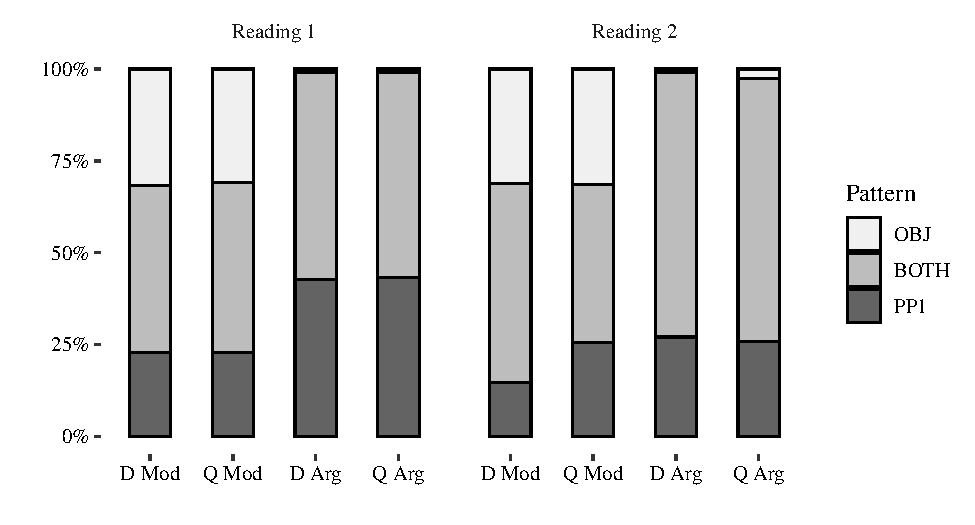
\includegraphics{99-append_files/figure-latex/bothbreaks2-1.pdf}
\caption{\label{fig:bothbreaks2}Figure: Break pattern as a function of sentence type and Reading.}
\end{figure}

\hypertarget{references}{%
\chapter*{References}\label{references}}
\addcontentsline{toc}{chapter}{References}

\noindent
\vspace{-2em}
\setlength{\parindent}{-0.5in}
\setlength{\leftskip}{0.5in}
\setlength{\parskip}{15pt}

\hypertarget{refs}{}
\leavevmode\hypertarget{ref-ashby2012eye}{}%
Ashby, J., Yang, J., Evans, K. H., \& Rayner, K. (2012). Eye movements and the perceptual span in silent and oral reading. \emph{Attention, Perception, and Psychophysics}, \emph{74}(4), 634--640.

\leavevmode\hypertarget{ref-Bader1998-ts}{}%
Bader, M. (1998). Prosodic influences on reading syntactically ambiguous sentences. In \emph{Reanalysis in sentence processing} (pp. 1--46). Springer.

\leavevmode\hypertarget{ref-R-lme4}{}%
Bates, D., Maechler, M., Bolker, B., \& Walker, S. (2019). \emph{Lme4: Linear mixed-effects models using 'eigen' and s4}. Retrieved from \url{https://CRAN.R-project.org/package=lme4}

\leavevmode\hypertarget{ref-Beckman1997-eu}{}%
Beckman, M. E., \& Ayers, G. (1997). Guidelines for ToBI labelling. \emph{The OSU Research Foundation}, \emph{3}, 30.

\leavevmode\hypertarget{ref-bever1970}{}%
Bever, T. G. (1970). The cognitive basis for linguistic structures. \emph{Cognition and the Development of Language}, \emph{279}(362), 1--61.

\leavevmode\hypertarget{ref-agreements}{}%
Breen, M., Dilley, L. C., Kraemer, J., \& Gibson, E. (2012). \emph{Inter-transcriber reliability for two systems of prosodic annotation: ToBI (tones and break indices) and rap (rhythm and pitch)}.

\leavevmode\hypertarget{ref-choi2005finding}{}%
Choi, J.-Y., Hasegawa-Johnson, M., \& Cole, J. (2005). Finding intonational boundaries using acoustic cues related to the voice source. \emph{The Journal of the Acoustical Society of America}, \emph{118}(4), 2579--2587.

\leavevmode\hypertarget{ref-chomsky2014minimalist}{}%
Chomsky, N. (2014). \emph{The minimalist program}. MIT press.

\leavevmode\hypertarget{ref-clifton1988restrictions}{}%
Clifton, C., Jr. (1988). Restrictions on late closure: Appearance and reality. \emph{6th australian language and speech conference}, 19--21.

\leavevmode\hypertarget{ref-cliftonEtAl1991}{}%
Clifton, C., Jr., Speer, S., \& Abney, S. P. (1991). Parsing arguments: Phrase structure and argument structure as determinants of initial parsing decisions. \emph{Journal of Memory and Language}, \emph{30}(2), 251--271.

\leavevmode\hypertarget{ref-lengthCCFL}{}%
Clifton, C., Carlson, K., \& Frazier, L. (2006). Tracking the what and why of speakers' choices: Prosodic boundaries and the length of constituents. \emph{Psychonomic Bulletin \& Review}, \emph{13}(5), 854--861.

\leavevmode\hypertarget{ref-Cuetos1988-tm}{}%
Cuetos, F., \& Mitchell, D. C. (1988). Cross-linguistic differences in parsing: Restrictions on the use of the late closure strategy in spanish. \emph{Cognition}, \emph{30}(1), 73--105.

\leavevmode\hypertarget{ref-den2006relators}{}%
Den Dikken, M. (2006). \emph{Relators and linkers: The syntax of predication, predicate inversion, and copulas} (Vol. 47). MIT press.

\leavevmode\hypertarget{ref-nazik}{}%
Dinçtopal Deniz, N., \& Fodor, J. D. (2017). Phrase lengths and the perceived informativeness of prosodic cues in turkish. \emph{Language and Speech}, \emph{60}(4), 505--529.

\leavevmode\hypertarget{ref-cps}{}%
Drury, J. E., Baum, S. R., Valeriote, H., \& Steinhauer, K. (2016). Punctuation and implicit prosody in silent reading: An erp study investigating english garden-path sentences. \emph{Frontiers in Psychology}, \emph{7}, 1375.

\leavevmode\hypertarget{ref-gmm1}{}%
Falk, T. H., \& Chan, W.-Y. (2006). Nonintrusive speech quality estimation using gaussian mixture models. \emph{IEEE Signal Processing Letters}, \emph{13}(2), 108--111.

\leavevmode\hypertarget{ref-fiengo}{}%
Fiengo, R. (2007). \emph{Asking questions: Using meaningful structures to imply ignorance}. Oxford University Press.

\leavevmode\hypertarget{ref-Fodor2002-io}{}%
Fodor, J. D. (2002). Psycholinguistics cannot escape prosody. \emph{Proceedings of the speech prosody international conference}.

\leavevmode\hypertarget{ref-fodor2019center}{}%
Fodor, J. D., Macaulay, B., Ronkos, D., Callahan, T., \& Peckenpaugh, T. (2019). Center-embedded sentences: An online problem or deeper? In K. Carlson, C. C. Jr, \& J. D. Fodor" (Eds.), \emph{Grammatical approaches to language processing} (pp. 11--28). Springer.

\leavevmode\hypertarget{ref-Frazier1979-pb}{}%
Frazier, L. (1979). \emph{On comprehending sentences: Syntactic parsing strategies}.

\leavevmode\hypertarget{ref-frazier1996construal}{}%
Frazier, L., \& Clifton, C., Jr. (1996). \emph{Construal}. MIT Press.

\leavevmode\hypertarget{ref-frazier1978sausage}{}%
Frazier, L., \& Fodor, J. D. (1978). The sausage machine: A new two-stage parsing model. \emph{Cognition}, \emph{6}(4), 291--325.

\leavevmode\hypertarget{ref-geh}{}%
Gehrke, B. (2006). On directional readings of locative prepositions. \emph{Proceedings of console xiv}, 99--120.

\leavevmode\hypertarget{ref-goldman1961-pa}{}%
Goldman-Eisler, F. (1961). The distribution of pause durations in speech. \emph{Language and Speech}, \emph{4}(4), 232--237.

\leavevmode\hypertarget{ref-Hedberg2017-er}{}%
Hedberg, N., Sosa, J. M., \& Görgülü, E. (2017). The meaning of intonation in yes-no questions in american english: A corpus study.

\leavevmode\hypertarget{ref-jacewicz2010-sr}{}%
Jacewicz, E., Fox, R. A., \& Wei, L. (2010). Between-speaker and within-speaker variation in speech tempo of american english. \emph{The Journal of the Acoustical Society of America}, \emph{128}(2), 839--850.

\leavevmode\hypertarget{ref-kimball1973seven}{}%
Kimball, J. (1973). Seven principles of surface structure parsing in natural language. \emph{Cognition}, \emph{2}(1), 15--47.

\leavevmode\hypertarget{ref-Kjelgaard1999-xd}{}%
Kjelgaard, M. M., \& Speer, S. R. (1999). Prosodic facilitation and interference in the resolution of temporary syntactic closure ambiguity.

\leavevmode\hypertarget{ref-n400}{}%
Kutas, M., Van Petten, C. K., \& Kluender, R. (2006). Psycholinguistics electrified ii (1994--2005). In \emph{Handbook of psycholinguistics} (pp. 659--724). Elsevier.

\leavevmode\hypertarget{ref-ladd}{}%
Ladd, D. R. (2008). \emph{Intonational phonology}. Cambridge University Press.

\leavevmode\hypertarget{ref-evs}{}%
Laubrock, J., \& Kliegl, R. (2015). The eye-voice span during reading aloud. \emph{Frontiers in Psychology}, \emph{6}(1432). \url{https://doi.org/10.3389/fpsyg.2015.01432}

\leavevmode\hypertarget{ref-os2012}{}%
Mathôt, S., Schreij, D., \& Theeuwes, J. (2012). OpenSesame: An open-source, graphical experiment builder for the social sciences. \emph{Behavior Research Methods}, \emph{44}(2), 314--324. \url{https://doi.org/10.3758/s13428-011-0168-7}

\leavevmode\hypertarget{ref-maynell1999effect}{}%
Maynell, L. A. (1999). Effect of pitch accent placement on resolving relative clause ambiguity in english. \emph{Poster presented at the 12th annual cuny conference on human sentence processing, new york}, 18--20.

\leavevmode\hypertarget{ref-spanmcr}{}%
McConkie, G. W., \& Rayner, K. (1975). The span of the effective stimulus during a fixation in reading. \emph{Perception \& Psychophysics}, \emph{17}(6), 578--586.

\leavevmode\hypertarget{ref-mehler1963some}{}%
Mehler, J. (1963). Some effects of grammatical transformations on the recall of english sentences. \emph{Journal of Verbal Learning and Verbal Behavior}, \emph{2}(4), 346--351.

\leavevmode\hypertarget{ref-p600}{}%
Neville, H., Nicol, J. L., Barss, A., Forster, K. I., \& Garrett, M. F. (1991). Syntactically based sentence processing classes: Evidence from event-related brain potentials. \emph{Journal of Cognitive Neuroscience}, \emph{3}(2), 151--165.

\leavevmode\hypertarget{ref-qp2}{}%
Peckenpaugh, T. (2016). \emph{Interrogative context and PP-attachment ambiguities}.

\leavevmode\hypertarget{ref-pynte1996prosodic}{}%
Pynte, J., \& Prieur, B. (1996). Prosodic breaks and attachment decisions in sentence parsing. \emph{Language and Cognitive Processes}, \emph{11}, 165--191.

\leavevmode\hypertarget{ref-raynerEtAl1983}{}%
Rayner, K., Carlson, M., \& Frazier, L. (1983). The interaction of syntax and semantics during sentence processing: Eye movements in the analysis of semantically biased sentences. \emph{Journal of Verbal Learning and Verbal Behavior}, \emph{22}(3), 358--374.

\leavevmode\hypertarget{ref-rayner2012psychology}{}%
Rayner, K., Pollatsek, A., Ashby, J., \& Clifton, C., Jr. (2012). \emph{Psychology of reading}. Psychology Press.

\leavevmode\hypertarget{ref-andrew}{}%
Rosenberg, A. (2009). \emph{Automatic detection and classification of prosodic events}. Columbia University.

\leavevmode\hypertarget{ref-salverda2003role}{}%
Salverda, A. P., Dahan, D., \& McQueen, J. M. (2003). The role of prosodic boundaries in the resolution of lexical embedding in speech comprehension. \emph{Cognition}, \emph{90}(1), 51--89.

\leavevmode\hypertarget{ref-schafer2000intonational}{}%
Schafer, A. J., Speer, S. R., Warren, P., \& White, S. D. (2000). Intonational disambiguation in sentence production and comprehension. \emph{Journal of Psycholinguistic Research}, \emph{29}(2), 169--182.

\leavevmode\hypertarget{ref-p600addscps}{}%
Steinhauer, K. (2003). Electrophysiological correlates of prosody and punctuation. \emph{Brain and Language}, \emph{86}(1), 142--164.

\leavevmode\hypertarget{ref-streeter1978acoustic}{}%
Streeter, L. A. (1978). Acoustic determinants of phrase boundary perception. \emph{The Journal of the Acoustical Society of America}, \emph{64}(6), 1582--1592.

\leavevmode\hypertarget{ref-webman2016phrase}{}%
Webman-Shafran, R., \& Fodor, J. D. (2016). Phrase length and prosody in on-line ambiguity resolution. \emph{Journal of Psycholinguistic Research}, \emph{45}(3), 447--474.


\end{document}
